\documentclass{beamer}

\usepackage{graphicx}
\usepackage{hyperref}
\usepackage[utf8]{inputenc}
\usepackage[german,english]{babel}
\usepackage[T1]{fontenc}
%\usepackage[english]{babel}
\usepackage{listings}
\usepackage{xcolor,url}
\usepackage{amssymb}
\usepackage{amsmath}
\usepackage{amsfonts}
\usepackage{mathtools}
\usepackage{ifthen}
\usepackage{tcolorbox}
\usepackage{tikz}
\usetikzlibrary{plotmarks}
\usepackage{pgfplots}
\usepackage{upgreek}
\usepackage{dsfont}
\usepackage{framed, color}

\usepackage{metricsbeamer} % using the metric beamer style

\DeclareMathAlphabet{\mathcalbf}{OMS}{cmsy}{b}{n}
%\newcommand{\dd}{\text{d}}
\newcommand{\del}{\partial}

% The command to define a subsection is '\subsec{}' and NOT '\subsection'.
% This code generates the bar. Don't edit.
\newcommand{\midbarnew}{}
\newcommand{\subsec}[1]
{
  \ifthenelse{\equal{#1}{}}
  {\renewcommand{\midbarnew}{} \subsection{}}
  {\renewcommand{\midbarnew}{ $\mid$ } \subsection{#1}}
}

% change the pictures here, if necessary. logobig and logosmall are the internal names
% for the pictures: do not modify them, just change "hulogo" and "logo". Pictures must be 
% supplied as JPEG, PNG or PDF
%########################################

\pgfdeclareimage[height=2cm]{logobig}{hulogo} % use hucase instead for the Humboldt-Case Logo
\pgfdeclareimage[height=1cm]{logosmall}{hulogo}

% use this number to modify the scaling of the headline on titlepage
\def\titlescale{1.3}


\def\authora{Philipp Töpfer}	% First Author
%\def\affa{Humboldt-Universität zu Berlin, Institut für Physik} % First Author's Affiliation
\def\authorb{Dr. Valentina Forini}  % Second Author
%\def\affb{Humboldt-Universität zu Berlin} % Second Author's Affiliation
\def\authorc{Dr. Björn Leder}  % Third Author
%\def\affc{Humboldt-Universität zu Berlin} % Third Author's Affiliation

\def\linka{}	% Link to your institution's/ personal website
\def\linkb{}
\def\linkc{}
\def\email{\href{mailto:your.email@address.com}{your.email@address.com}}	% Your email address

\title[Strings on the lattice and AdS/CFT]{\centering Lattice discretisation of the Green-Schwarz superstring and AdS/CFT \\}
\institute{Humboldt-Universität zu Berlin \\ Emmy Noether Research Group}

% - - - - - - - - - - - - - - - - - - - - - - - - - - - - - - - - - -


%Start of the document
\begin{document}
\Section{}

\frame[plain]{% create the titleslide, layout controlled in metricsbeamer
\vspace{-1.5cm}	\titlepage
}

\Section{Introduction}

\frame{% how to print
\frametitle{Outline}

\begin{tcolorbox}[colback=white!95!black, colframe=white!90!black]
\begin{center}
\textcolor{blue!90}{Lattice} field theory study of \textcolor{blue!90}{AdS/CFT} from a \textcolor{blue!90}{worldsheet string perspective}
\end{center}
\end{tcolorbox}
\hfill \vspace{1mm}



\begin{itemize}
\item<2-> Motivation
\item<2-> AdS/CFT duality
\item<2-> String theory framework
\item<2-> Numerical approach
\item<2-> Results and conclusion
\end{itemize}

}

%###############################################

\Section{Motivation}

%\frame{
%\frametitle{Motivation}
%
%\begin{itemize}
%\item<1-> Good predictions on the real world via QCD
%\item<1-> Fundamental aim: particle masses as functions of parameters\\
%\begin{center} $m_{\rm p} = f(\alpha_{\rm s},\alpha,\mu_{\rm reg},\ldots)$ \end{center}
%\item<2-> Gain more insights on QCD $\leftrightarrow$ study more symmetric model %($\mathcal{N}=4$ SYM)
%\item<2-> $\mathcal{N}=4$ SYM: 
%\begin{itemize}
%\item no massive particles
%\item measure scaling dimensions of local operators and Wilson loops
%\end{itemize}
%\item<3-> Twist two operators:\\
%scaling dimension $\Delta_{S} = 2+S+ \gamma_{S}$\\
%twist \hspace{19mm} $\Delta_{S}-S = 2+ \gamma_{S}$
%\end{itemize}
%}

\begin{frame}
\frametitle{Motivation}
\begin{itemize}
\item Standard Model is most efficient theory of particle physics
\begin{itemize}
\item Unable to incorporate gravity
\item Study $\mathcal{N}=4$ SYM (superconformal version of QCD)
\end{itemize}
\item One of most remarkable discoveries in last decades:\\
{\bf AdS/CFT correspondence} [Maldacena 1997]
\begin{itemize}
\item Relates a superconformal field theory (like $\mathcal{N}=4$ SYM) to a string theory
\item Strong/weak coupling duality
\end{itemize}
\item Study AdS/CFT via the cusp anomaly function ${\color{blue}f(g)}$ from $\mathcal{N}=4$ SYM
\end{itemize}
\end{frame}

%################################################

{\subsec{Cusp anomaly function}

%\begin{frame}
%% mp left
%\begin{minipage}[t]{0.5\linewidth}
%\begin{tcolorbox}[colback=white!95!black, colframe=white!90!black]
%\begin{center}
%\vspace{2.5mm}
%Wilson loop with cusp
%\vspace{2mm}
%\end{center}
%\end{tcolorbox}
%%
%\begin{tcolorbox}[colback=white!95!black, colframe=white!90!black]
%\begin{center}
%$\langle \mathcal{W}[\mathcal{C_{\rm cusp}}]\rangle \sim e^{-\frac{\color{blue}{f(g)}}{2}\vert \phi\vert \ln \frac{L}{\epsilon}}$
%\end{center}
%\end{tcolorbox}
%\end{minipage}
%%
%% mp center
%%
%\begin{minipage}[t]{0.05\linewidth}
%\begin{center}
%\vspace{1.5mm}
%$\Leftrightarrow$
%\end{center}
%\end{minipage}
%%
%% mp right
%%
%\begin{minipage}[t]{0.4\linewidth}
%\begin{tcolorbox}[colback=white!95!black, colframe=white!90!black]
%\begin{center}
%anomalous dimension $\gamma_{S}$
%\end{center}
%\end{tcolorbox}
%%
%\begin{tcolorbox}[colback=white!95!black, colframe=white!90!black]
%\begin{center}
%\vspace{1mm}
%$\gamma_{S} \simeq {\color{blue}f(g)} \ln S$
%\vspace{1mm}
%\end{center}
%\end{tcolorbox}
%\end{minipage}
%%
%%
%%
%\only<1>{
%\begin{center}
%\begin{tikzpicture}[thick,scale=0.5, every node/.style={scale=0.7}]
%\node[anchor=south west,inner sep=0] (image) at (0,0) {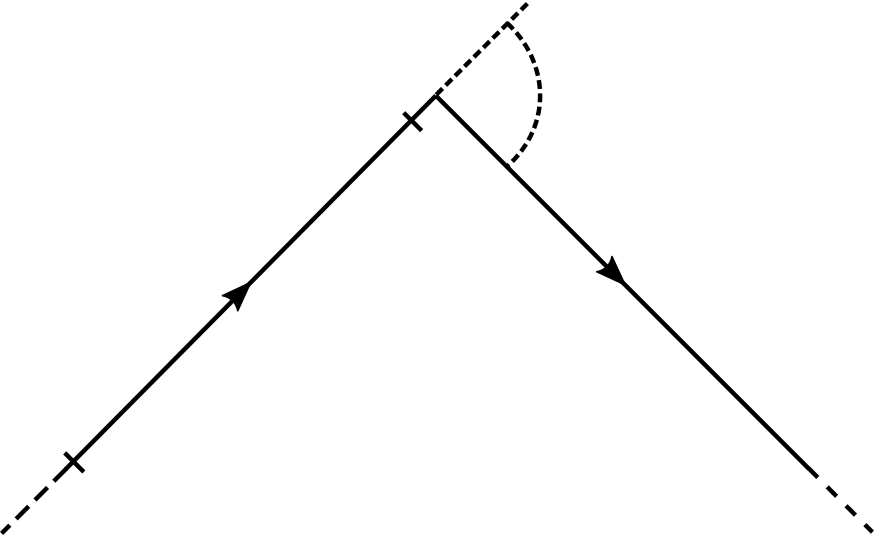
\includegraphics[width=0.8\textwidth]{W_cusp.png}};
%\begin{scope}[x={(image.south east)},y={(image.north west)}]
%\node [anchor=west] at (0.69,0.3) {$\mathcal{C_{\rm cusp}}$};
%\node [anchor=south] at (0.072,0.14) {$L$};
%\node [anchor=south] at (0.45,0.78) {$\epsilon$};
%\node [anchor=west] at (0.62,0.82) {$\phi$};
%%\draw[help lines,xstep=.1,ystep=.1] (0,0) grid (1,1);
%%\foreach \x in {0,1,...,9} { \node [anchor=north] at (\x/10,0) {0.\x}; }
%%\foreach \y in {0,1,...,9} { \node [anchor=east] at (0,\y/10) {0.\y}; }
%\end{scope}
%\end{tikzpicture}
%\end{center}
%}
%%
%%
%\only<2>{
%\begin{center}
%via cusp anomaly function
%\end{center}
%\begin{minipage}{0.65\linewidth}
%\begin{tikzpicture}[thick,scale=0.5, every node/.style={scale=0.7}]
%\node[anchor=south west,inner sep=0] (image) at (0,0) {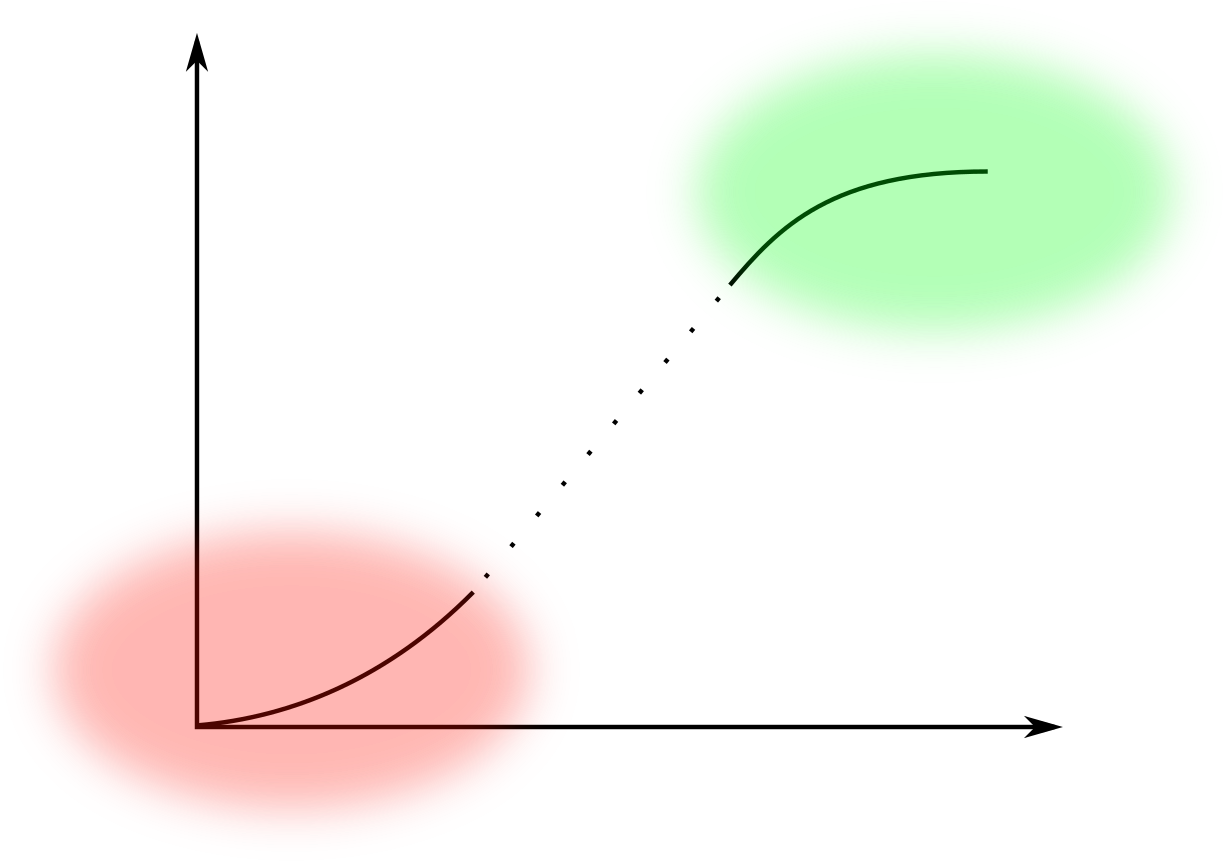
\includegraphics[width=1.1\textwidth]{cusp_anom.png}};
%\begin{scope}[x={(image.south east)},y={(image.north west)}]
%\node [anchor=east] at (0.15,0.92) {$\color{blue} f(g)$};
%\node [anchor=north] at (0.85,0.15) {$\color{blue} g$};
%\node [anchor=south] at (0.75,0.8) {\footnotesize pert. string $\sigma$-model};
%\node [anchor=north] at (0.22,0.17) {\footnotesize pert. gauge theory};
%\node [anchor=east] at (0.5,0.6) {\textcolor{red}{\footnotesize Integrability}};
%\node [anchor=west] at (0.5,0.5) {\textcolor{red}{\footnotesize non-pert. methods}};
%%\draw[help lines,xstep=.1,ystep=.1] (0,0) grid (1,1);
%%\foreach \x in {0,1,...,9} { \node [anchor=north] at (\x/10,0) {0.\x}; }
%%\foreach \y in {0,1,...,9} { \node [anchor=east] at (0,\y/10) {0.\y}; }
%\end{scope}
%\end{tikzpicture}
%\end{minipage}
%%
%%
%\begin{minipage}{0.3\linewidth}
%Here ${\color{blue}g} \equiv \frac{\sqrt{\lambda}}{4\pi} $ \\[3mm]
%t'Hooft coupling\\[2mm]
%$\lambda = g_{\rm YM}^{2}N = \frac{R^{4}}{\alpha'^{2}}$
%
%\end{minipage}
%}
%\end{frame}

\begin{frame}
\vspace{-2mm}
\begin{center}
Cusp anomaly function
\end{center}
\begin{minipage}{0.65\linewidth}
\begin{tikzpicture}[thick,scale=0.5, every node/.style={scale=0.7}]
\node[anchor=south west,inner sep=0] (image) at (0,0) {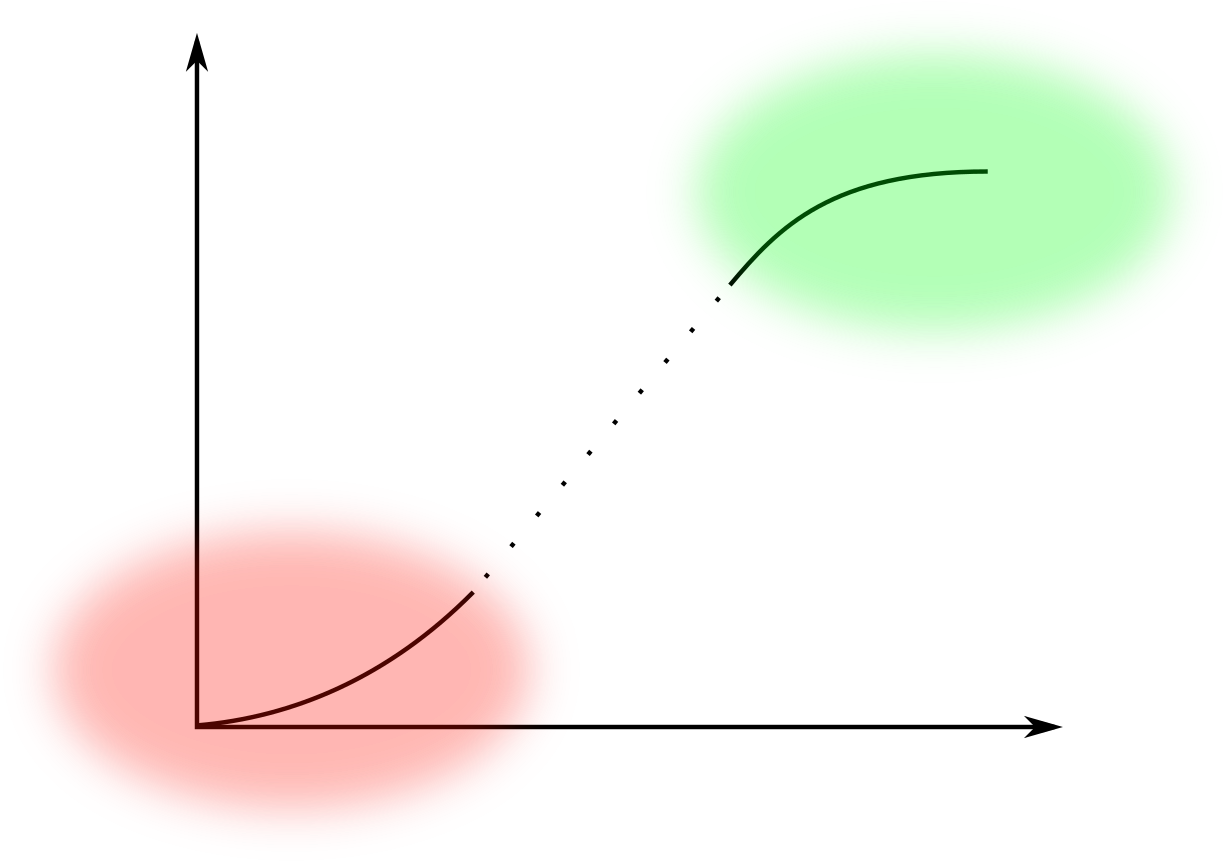
\includegraphics[width=1.1\textwidth]{cusp_anom.png}};
\begin{scope}[x={(image.south east)},y={(image.north west)}]
\node [anchor=east] at (0.15,0.92) {$\color{blue} f(g)$};
\node [anchor=north] at (0.85,0.15) {$\color{blue} g$};
\node [anchor=south] at (0.75,0.8) {\footnotesize pert. string $\sigma$-model};
\node [anchor=north] at (0.22,0.17) {\footnotesize pert. gauge theory};
\node [anchor=east] at (0.5,0.6) {\textcolor{red}{\footnotesize Integrability}};
\node [anchor=west] at (0.5,0.5) {\textcolor{red}{\footnotesize non-pert. methods}};
%\draw[help lines,xstep=.1,ystep=.1] (0,0) grid (1,1);
%\foreach \x in {0,1,...,9} { \node [anchor=north] at (\x/10,0) {0.\x}; }
%\foreach \y in {0,1,...,9} { \node [anchor=east] at (0,\y/10) {0.\y}; }
\end{scope}
\end{tikzpicture}
\end{minipage}
%
%
\begin{minipage}{0.3\linewidth}
Here ${\color{blue}g} \equiv \frac{\sqrt{\lambda}}{4\pi} $ \\[3mm]
t'Hooft coupling\\[2mm]
$\lambda = g_{\rm YM}^{2}N = \frac{R^{4}}{\alpha'^{2}}$

\end{minipage}
\par
\vspace{2mm}
%Investigate cusp anomaly of $\mathcal{N}=4$ SYM from string theory perspective\\[2mm]
%solve non-trivial 4d QFT with SUSY $\xrightarrow{\color{red} AdS/CFT}{}$ solve non-trivial 2d QFT
\begin{itemize}
\item[] Numerical investigation:\\[2mm]
\begin{minipage}{0.38\linewidth}
\begin{center}
\small solve non-trivial 4d QFT with SUSY
\end{center}
\end{minipage}
\begin{minipage}{0.18\linewidth}
$\xrightarrow{\color{red} AdS/CFT}{}$
\end{minipage}
\begin{minipage}{0.38\linewidth}
\small solve non-trivial 2d QFT
\end{minipage}
\vspace{2mm}
\begin{itemize}
\item More economic memory consumption 
\item Green-Schwarz (GS) approach inherits supersymmetry
\item Only scalar fields involved
\end{itemize}
\end{itemize}
\end{frame}
}

%################################################

\Section{AdS/CFT duality}
\frame{
\frametitle{AdS/CFT duality}

\begin{tcolorbox}[colback=white!95!black, colframe=white!90!black]
\begin{center}
conformal field theory (CFT)
\end{center}
\end{tcolorbox}
%
\begin{equation*}
\uparrow \qquad \textit{dynamically equivalent to} \qquad \downarrow
\end{equation*}\hspace{1mm}
%
%
\begin{tcolorbox}[colback=white!95!black, colframe=white!90!black]
\begin{center}
string theory on background containing Anti-de Sitter (AdS) space as a factor
\end{center}
\end{tcolorbox}

}

%############################################

\frame{
\textbf{Most symmetric setting similar to QCD:} \\[0.3cm]

\begin{tcolorbox}[colback=white!95!black, colframe=white!90!black]
\begin{minipage}{0.70\linewidth}
\begin{center}
\textbf{$\mathcalbf{N}=\mathbf{4}$ SYM}\\
 in 4d, $( g_{\rm YM}, N)$
\end{center}
\end{minipage}
\begin{minipage}{0.20\linewidth}
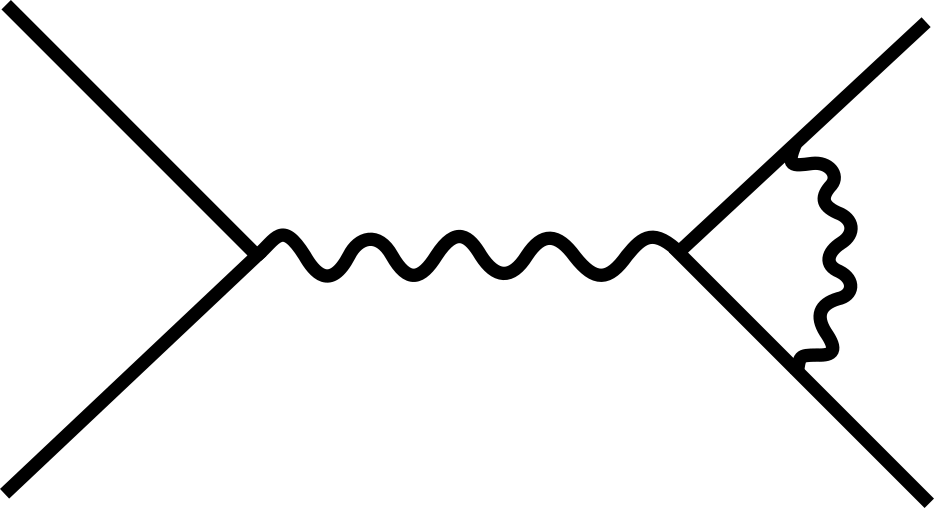
\includegraphics[scale=0.15]{feynm.png}
\end{minipage}


\end{tcolorbox}
%
\begin{equation*}
\uparrow \qquad \textit{dynamically equivalent to} \qquad \downarrow
\end{equation*}\hspace{1mm}
%
%
\begin{tcolorbox}[colback=white!95!black, colframe=white!90!black]
\begin{minipage}{0.65\linewidth}
\begin{center}
\textbf{Type IIB superstring theory}\\
on $AdS_{5}\times S^{5}$,  $(g_{\rm s},R)$
\end{center}
\end{minipage}
\begin{minipage}{0.15\linewidth}
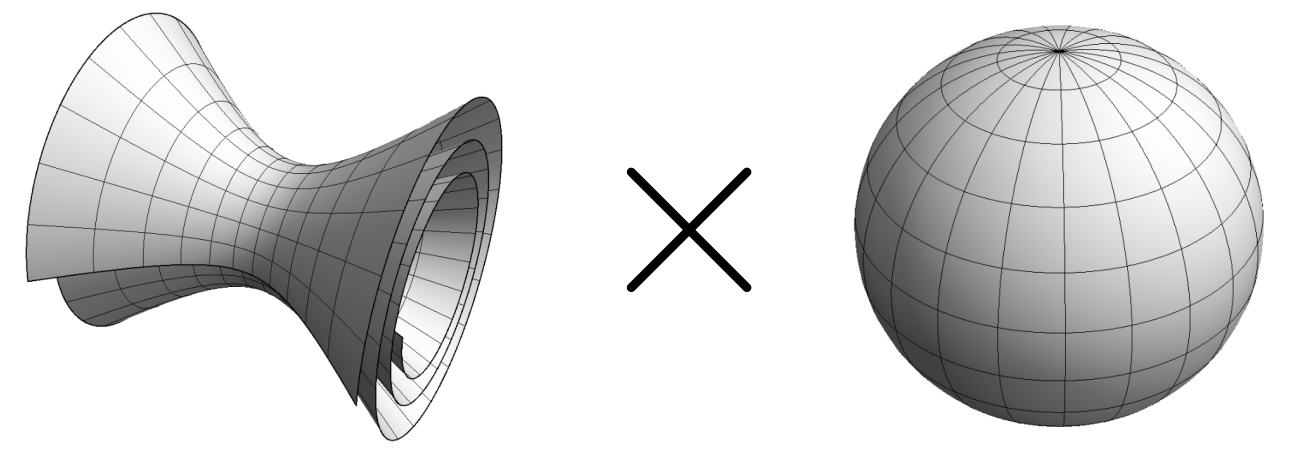
\includegraphics[scale=0.15]{AdS_S.png}
\end{minipage}
\end{tcolorbox}

}

%##############################################

\frame{
\begin{minipage}{0.25\linewidth}
\begin{tcolorbox}[colback=white!95!black, colframe=white!90!black]
\begin{center}\vspace{3mm}
\textbf{$\mathcalbf{N}=\mathbf{4}$ SYM}
\vspace{3mm}
\end{center}
\end{tcolorbox}
%
%
\begin{tcolorbox}[colback=white!90!red, colframe=white!90!black]
\begin{center}
\vspace{5mm}
$\Uparrow$\\
\textbf{AdS/CFT}\\
$\Downarrow$\\
\vspace{5mm}
\end{center}
\end{tcolorbox}
%
%
\begin{tcolorbox}[colback=white!95!black, colframe=white!90!black]
\begin{center}
\textbf{Type IIB strings}
\end{center}
\end{tcolorbox}
\end{minipage}
%
%
%
\begin{minipage}{0.73\linewidth}
\begin{tcolorbox}[colback=white!95!blue, colframe=white!90!black]
\begin{center}
Wilson loop
\end{center}
$\langle \mathcal{W}[\mathcal{C}]\rangle = \frac{1}{N}{\rm Tr}\,\mathcal{P}\,e^{\oint \left(iA_{\mu}\dot{x}^{\mu}+\phi_{i}\dot{y}^{i}\right) {\rm d}s }$
\end{tcolorbox}
\begin{center}
\begin{tikzpicture}[thick,scale=0.5, every node/.style={scale=0.7}]
\node[anchor=south west,inner sep=0] (image) at (0,0) {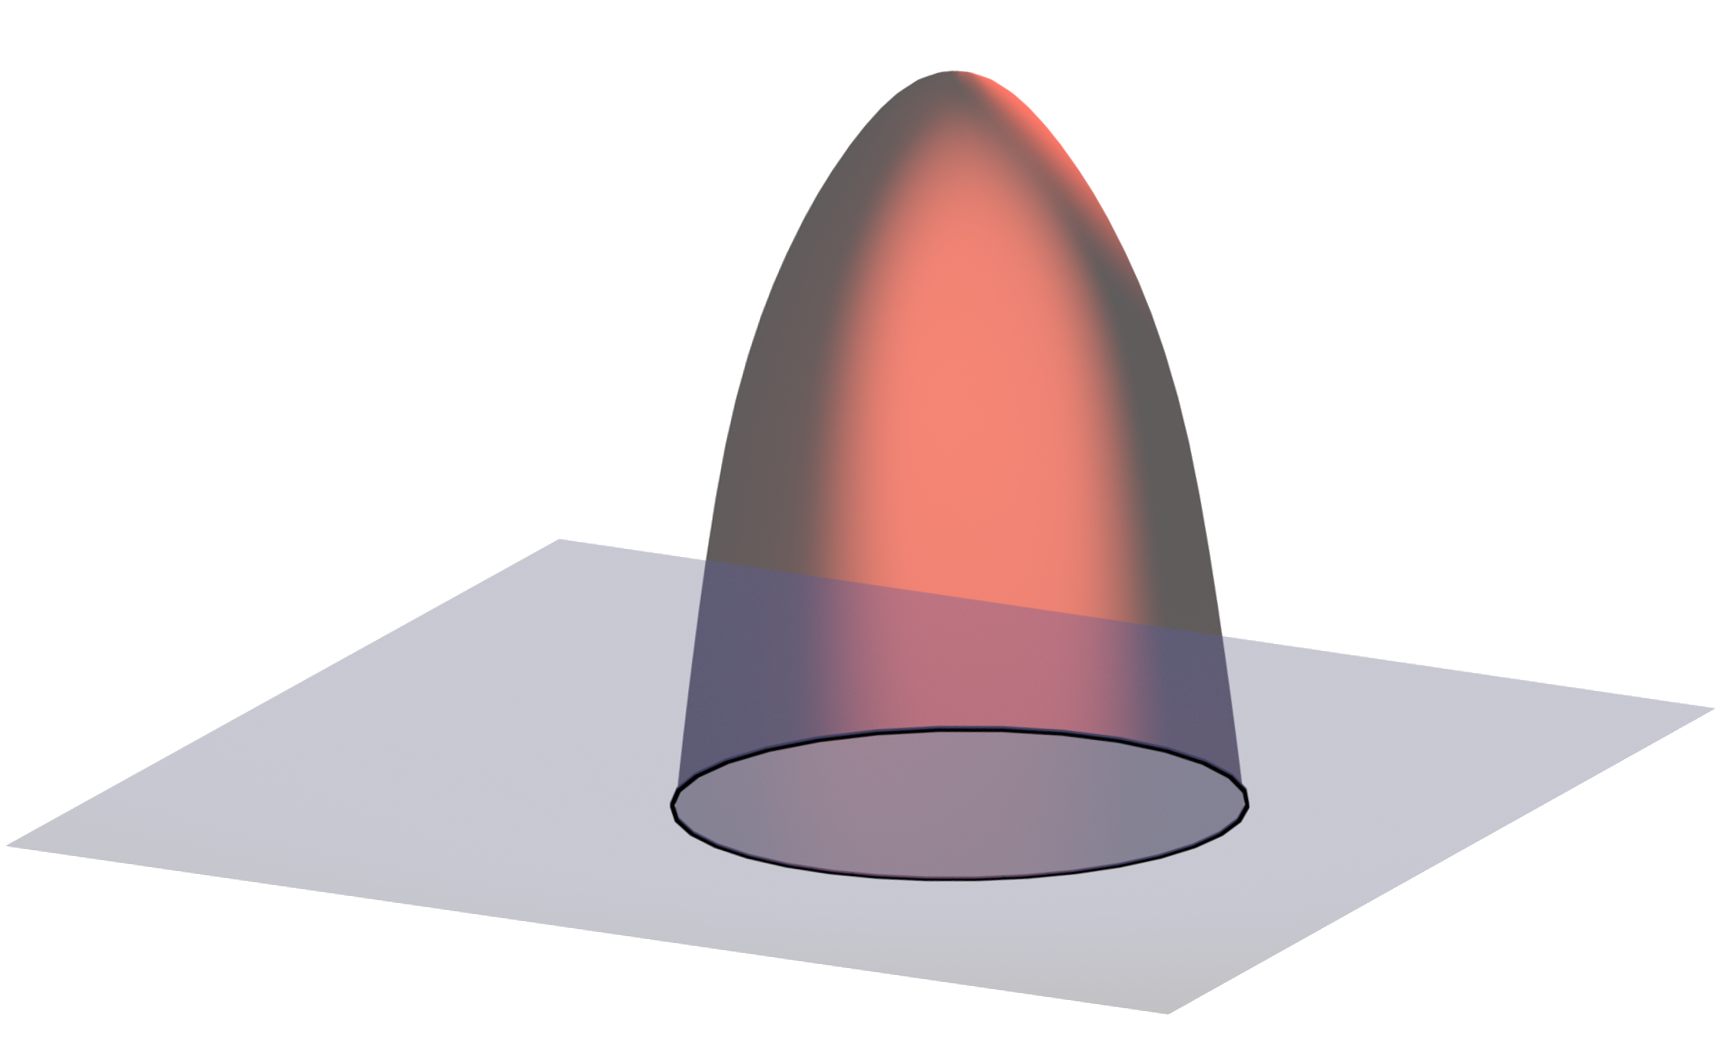
\includegraphics[width=0.7\textwidth]{Wilson_loop_worldsheet1.png}};
\begin{scope}[x={(image.south east)},y={(image.north west)}]
\node [anchor=west] at (0.6,0.1) {$\mathcal{C}$};
%\node [anchor=west] at (0.8,0.6) {$\widetilde{\Sigma}$};
%\node [anchor=west] at (0.95,0.1) {$z$};
%\draw[help lines,xstep=.1,ystep=.1] (0,0) grid (1,1);
%\foreach \x in {0,1,...,9} { \node [anchor=north] at (\x/10,0) {0.\x}; }
%\foreach \y in {0,1,...,9} { \node [anchor=east] at (0,\y/10) {0.\y}; }
\end{scope}
\end{tikzpicture}
\end{center}
%
%
%
\begin{tcolorbox}[colback=white!95!blue, colframe=white!90!black]
\vspace{1mm}
${\!\!Z_{\rm string}[\mathcal{C}]\!=\! \int \mathcal{D}X\mathcal{D}h\, e^{-S_{\rm string}(X,h)} \!\sim\! e^{-A_{\rm reg}(\mathcal{C})}}$\\
\vspace{-1mm}
\end{tcolorbox}
\end{minipage}

}

%###############################################

\frame{
\frametitle{Cusp anomaly of $\mathcalbf{N}=\mathbf{4}$ SYM from string theory}
\begin{minipage}{0.6\linewidth}
vev of light-like cusped Wilson loop\\
\begin{tcolorbox}[colback=white!95!black, colframe=white!90!black]
${\!\!\!\langle\mathcal{W}[\mathcal{C}_{\rm cusp}]\rangle \sim e^{-\frac{f(g)}{2}\vert\phi\vert \ln \frac{L}{\epsilon}}, \quad \phi\to\infty}$
\end{tcolorbox}
\end{minipage}
%
\begin{minipage}{0.35\linewidth}
\begin{flushright}
%\begin{tikzpicture}[thick,scale=0.9, every node/.style={scale=0.7}]
%\node[anchor=south west,inner sep=0] (image) at (0,0) {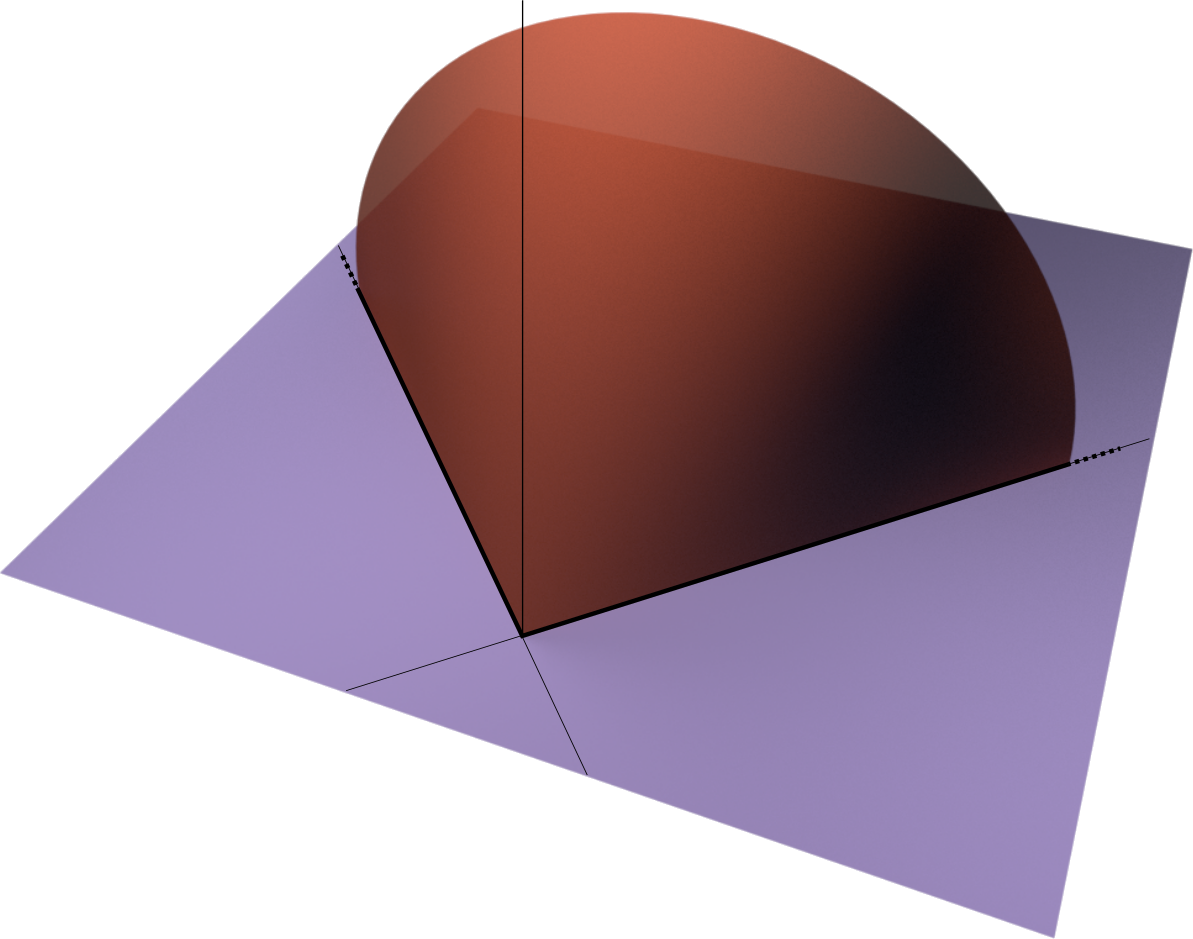
\includegraphics[width=1.2\textwidth]{cusp_worldsheet_vec.png}};
%\begin{scope}[x={(image.south east)},y={(image.north west)}]
%\node [anchor=north] at (0.6,0.37) {$\mathcal{C}_{\rm cusp}$};
%%\draw[help lines,xstep=.1,ystep=.1] (0,0) grid (1,1);
%%\foreach \x in {0,1,...,9} { \node [anchor=north] at (\x/10,0) {0.\x}; }
%%\foreach \y in {0,1,...,9} { \node [anchor=east] at (0,\y/10) {0.\y}; }
%\end{scope}
%\end{tikzpicture}
\vspace{3mm}
\begin{tikzpicture}[thick,scale=0.8, every node/.style={scale=0.7}]
\node[anchor=south west,inner sep=0] (image) at (0,0) {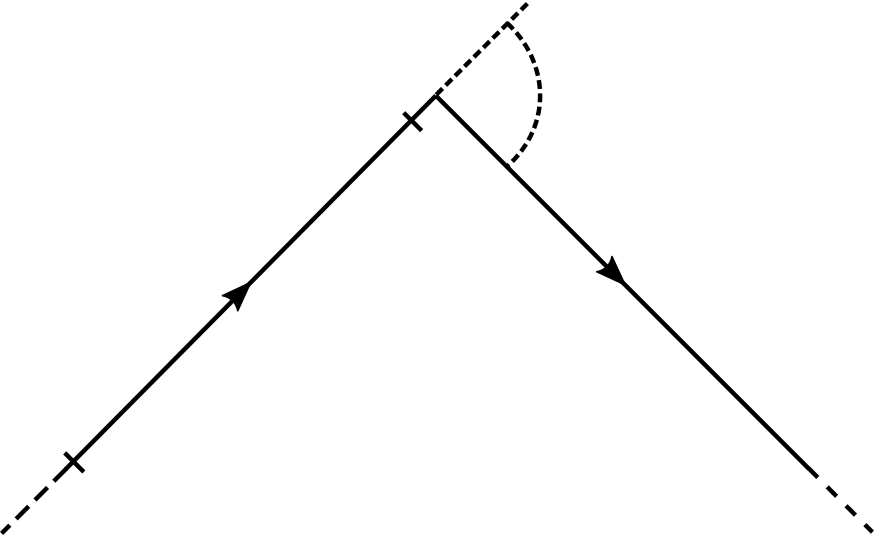
\includegraphics[width=1.5\textwidth]{W_cusp.png}};
\begin{scope}[x={(image.south east)},y={(image.north west)}]
\node [anchor=west] at (0.64,0.3) {$\mathcal{C_{\rm cusp}}$};
\node [anchor=south] at (0.072,0.14) {$L$};
\node [anchor=south] at (0.45,0.78) {$\epsilon$};
\node [anchor=west] at (0.62,0.82) {$\mathit{\Phi}=i\phi$};
%\draw[help lines,xstep=.1,ystep=.1] (0,0) grid (1,1);
%\foreach \x in {0,1,...,9} { \node [anchor=north] at (\x/10,0) {0.\x}; }
%\foreach \y in {0,1,...,9} { \node [anchor=east] at (0,\y/10) {0.\y}; }
\end{scope}
\end{tikzpicture}
\end{flushright}
\end{minipage}
%
\begin{center}
$\Updownarrow$  \textcolor{red}{AdS/CFT}
\end{center}
%
\begin{tcolorbox}[colback=white!95!black, colframe=white!90!black]
$Z_{\rm cusp} = \int \mathcal{D}\delta X \, \mathcal{D}\delta \mathit{\Psi}\; e^{-S_{\rm IIB}(X_{\rm cl}+\delta X, \delta \mathit{\Psi})} = e^{-\frac{f(g)}{2}\frac{V_{2}}{4}}$
\end{tcolorbox}
String partition function with cusp vacuum $\left( V_{2}=\int {\rm d}t{\rm d}s \right)$

}

%##############################################################

\Section{String theory framework}

\frame{
\frametitle{Green-Schwarz string in AdS light-cone gauge}

\begin{itemize}
\item Sigma-model in $AdS_{5}\times S^{5}$ with RR flux\vspace{2mm}
$S = g \int \dd\tau \dd \sigma\,\left[ G \del X \cdot \del X + \bar{\!\mathit{\Theta}} \Gamma (D+F_{5}) \mathit{\Theta}\del X + \ldots \right]$
\vspace{1mm}
\begin{flushright}
\footnotesize [Metsaev Tseytlin 1998]
\end{flushright}
%
\begin{itemize}
\item $X^{\mu}$ - coordinates of 10d target space
\item $\mathit{\Theta}^{1},\, \mathit{\Theta}^{2}$ - anti-commuting Majorana-Weyl spinors
\end{itemize}

\item Fix $\kappa$-symmetry and apply bosonic light-cone gauge \\
$\Rightarrow$ action at most quartic in complex Grassmann fields $\theta^{i}, \eta^{i}$ (remnants of $\mathit{\Theta}$)

\end{itemize}
}

%###############################################################
%
%\begin{frame}
%\frametitle{Linearisation of fermions}
%quartic fermion contributions $\to \mathit{\Psi}^T \mathcal{O}_{\rm F} \mathit{\Psi}$\\
%Apply a Hubbard-Stratonovich transformation\\
%
%\end{frame}
%
%###############################################################

\begin{frame}
\frametitle{Green-Schwarz string in null-cusp background}

\begin{itemize}
\item In Poincaré patch\vspace{2mm}
$\dd s^{2}_{AdS_{5}} = \frac{\dd z^{2} + \dd x^{+}\dd x^{-} + \dd x^{*}\dd x}{z^{2}}, \quad x^{\pm}=x^{3}\pm x^{0}, \quad x=x^{1}+ix^{2}$\vspace{2mm}
classical solution $\big(\tau,\sigma \in (0,\infty)\big)$: surface\vspace{2mm}
\begin{center}
$z = \sqrt{\frac{\tau}{\sigma}},\quad x^{+}=\tau,\quad x^{-}= -\frac{1}{2\sigma}$ 
\end{center}
\vspace{2mm}
bounded by a null cusp \\ ($AdS_{5}$ boundary at $0=z^{2}=-2x^{+}x^{-}$)
%
\item Expand around classical solution + \\{\small $(\tau,\sigma) \to (t,s)=(\ln \tau,\ln \sigma)$}\\
\vspace{2mm}
{\small $S_{\rm cusp} = g\int \dd t\dd s\, \mathcal{L}_{\rm cusp}$}


\end{itemize}
\only<1>{
\vspace{-26mm}
%\begin{flushright}
\hspace{7.4cm}\begin{tikzpicture}[thick,scale=0.9, every node/.style={scale=0.7}]
\node[anchor=south west,inner sep=0] (image) at (0,0) {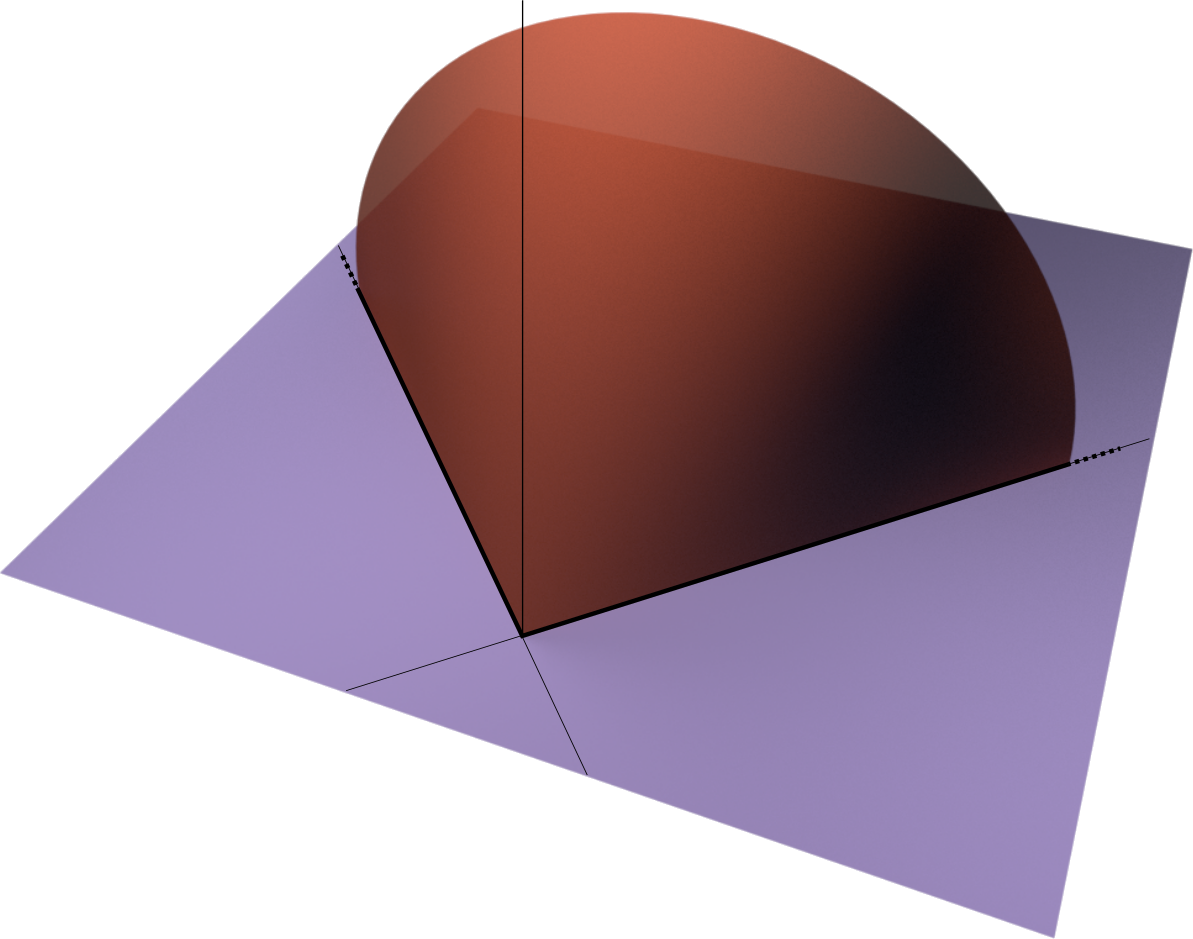
\includegraphics[width=0.5\textwidth]{cusp_worldsheet_vec.png}};
\begin{scope}[x={(image.south east)},y={(image.north west)}]
\node [anchor=north] at (0.6,0.37) {$\mathcal{C}_{\rm cusp}$};
\node [anchor=east] at (0.43,1.0) {$z$};
\node [anchor=east] at (0.28,0.75) {$x^{+}$};
\node [anchor=west] at (0.95,0.53) {$x^{-}$};
%\draw[help lines,xstep=.1,ystep=.1] (0,0) grid (1,1);
%\foreach \x in {0,1,...,9} { \node [anchor=north] at (\x/10,0) {0.\x}; }
%\foreach \y in {0,1,...,9} { \node [anchor=east] at (0,\y/10) {0.\y}; }
\end{scope}
\end{tikzpicture}
%\end{flushright}
	}
\end{frame} 

%########################################################

\frame{
\frametitle{Green-Schwarz string in null-cusp background}
\only<1>{
Linearising quartic fermion contributions with {\bf Hubbard-Stratonovich transformation}\\[4mm]
\begin{center}
{ $e^{-g \int \dd t \dd s [-\frac{1}{z^{2}}(-6(\eta^{2})^{2}-\cdots )]} \sim \int \mathcal{D}\phi \mathcal{D}\phi^{I} e^{-g\int \dd t \dd s [\frac{12}{z}\eta^{2}\phi +6\phi^{2} +\cdots] }$}
\end{center}
}


{\small \begin{align*}
\mathcal{L}_{\rm cusp} &=  {\left\vert \partial_t {x} + {\tfrac{m}{2}}{x} \right\vert}^2 + \tfrac{1}{{ z}^4}{\left\vert \partial_s {x} -\tfrac{m}{2}{x} \right\vert}^2 + \left(\partial_t {z}^M + \tfrac{m}{2}{z}^M \right)^2 \\ &\quad+ \frac{1}{{ z}^4} \left(\partial_s {z}^M -\tfrac{m}{2}{z}^M\right)^2
+ \phi^2 +\left( \phi_{I}\right)^{2} + \mathit{\Psi}^T \mathcal{O}_{\rm F} \mathit{\Psi} 
\end{align*}}

\only<1>{
\begin{itemize}
\item 8 bosonic coordinates: {\small $x,x^{*},z^{M}\;(M=1,\ldots,6),\; z=\sqrt{z_{M}z^{M}}$}
\item 17 auxiliary fields {\small $\phi, \phi_{I}$ \small $(I=1,\ldots,16)$}
\item 8 fermionic variables {\small $\mathit{\Psi} \equiv (\theta^{i},\theta_{i},\eta^{i},\eta_{i})$, $\theta^{i}=\theta_{i}^{\dagger}$, $\eta^{i}= \eta_{i}^{\dagger}$, $(i=1,\ldots,4)$}
\end{itemize}
	}
	
\only<2>{
{\footnotesize
\vspace{-8mm}
\begin{flalign*}
\!\!\!\!\!\!\!\!\!\!\!\!\!\!\!\!
\mathcal{O}_{\rm F} & =\begin{pmatrix}
0 & i \mathds{1}_{4}\partial_{t} &\!\!\!\!\! -i\rho^{M}\left(\partial_{s}+\frac{m}{2}\right)\frac{{z}^{M}}{{z}^{3}} & 0\\
i \mathds{1}_{4}\partial_{t} & 0 & 0 & \!\!\!\!\!-i\rho_{M}^{\dagger}\left(\partial_{s}+\frac{m}{2}\right)\frac{{z}^{M}}{{z}^{3}}\\
i\frac{{z}^{M}}{{z}^{3}}\rho^{M}\left(\partial_{s}-\frac{m}{2}\right) & 0 & \!\!\!\!\!2\frac{{z}^{M}}{{z}^{4}}\rho^{M}\left(\partial_{s}{x}-m\frac{{x}}{2}\right) & i \mathds{1}_{4}\partial_{t}-A^{T}\\
0 & \!\!\!\!\! i\frac{{z}^{M}}{{z}^{3}}\rho_{M}^{\dagger}\left(\partial_{s}-\frac{m}{2}\right) &i \mathds{1}_{4}\partial_{t}+A & \!\!\!\!\!\!\!\! -2\frac{{z}^{M}}{{z}^{4}}\rho_{M}^{\dagger}\left(\partial_{s}{x}^\ast-m\frac{{x}}{2}^\ast\right)
\end{pmatrix}~,
\raisetag{-8pt}
\end{flalign*}\\\vspace{2mm}
%
\small
$A=-\frac{\sqrt{6}}{z}\phi \mathds{1}_{4} + \frac{1}{z}\tilde{\phi}+\frac{1}{z^{3}}\rho^\ast_{N}\tilde{\phi}^{T}\rho^{L}z^{N}z^{L}+\mathrm{i}\frac{z^{N}}{z^2}\rho^{MN}\partial_{t}z^{M}$
}
	}	
	
}

%#################################################
\Section{Numerical approach}

\begin{frame}
\frametitle{Numerical approach}

Requires calculating expectation values\vspace{2mm}
{
%\begin{align*}
\begin{tcolorbox}[colback=white!95!black, colframe=white!90!black]
\begin{center}
$Z_{\rm cusp} = \int \mathcal{D}\delta X\mathcal{D}\delta \mathit{\Psi} \; e^{-S_{\rm cusp}} = e^{-\frac{f(g)}{2}\frac{V_{2}}{4}}$
\end{center}
\end{tcolorbox} %\\
\begin{center}
$\Downarrow \qquad \qquad \Downarrow$
\end{center}
\begin{tcolorbox}[colback=white!95!black, colframe=white!90!black]
\begin{align*}
\fcolorbox{white!70!black}{white!80!blue}{$\langle S_{\rm cusp} \rangle $} &= \frac{1}{Z_{\rm cusp}} \int \mathcal{D}\delta X\mathcal{D}\delta \mathit{\Psi} \; S_{\rm cusp} e^{-S_{\rm cusp}} \\
&= -g \frac{\dd \ln Z_{\rm cusp}}{\dd g} = \fcolorbox{white!70!black}{white!80!blue}{$g f'(g) \frac{V_{2}}{8}$}
\end{align*}
\end{tcolorbox}
}
\end{frame}

%########################################################

\begin{frame}
\frametitle{Lattice discretisation}
\begin{minipage}{0.65\linewidth}
\begin{tcolorbox}[colback=white!95!black, colframe=white!90!black]
{\small ${\!\!\!\!\!\!\!\langle A \rangle = \tfrac{1}{Z}\int \mathcal{D}\phi\, A[\phi]e^{-S[\phi]}, \quad Z=\int \mathcal{D}\phi\,e^{-S[\phi]}}$}
\end{tcolorbox}% \vspace{2mm}
Discretise the worldsheet with const. lattice spacing $a$ \\
{\small$\mathit{\Lambda}=\lbrace(n_{0},n_{1})\vert n_{\alpha}=0,\ldots,(N_{\alpha}-1)\rbrace$} so that {\small$\xi^{\alpha}=(t,s)\equiv (an_{0},an_{1}) \equiv an$}
\end{minipage}
\begin{minipage}{0.3\linewidth}
\only<1->{
\vspace{-1cm}
\begin{flushright}
\begin{tikzpicture}[scale=1.1]
%flat grid
\draw (-1,-1) rectangle (1,1);
\path (-1,-1) -- node[below]{$t$} (1,-1);
\path (-1,-1) -- node[left]{$s$} (-1,1);
\draw [step=0.5cm,dashed] (-1,-1) grid (1,1);
\node [anchor=north] at (-1,-1.0) {\tiny $a(0,0)$};
\node [anchor=north] at (1,-1.0) {\tiny $a(T-1,0)$};
\node [anchor=south] at (-1,1.0) {\tiny $a(0,L-1)$};
\path (0,0) circle (0.6pt) node[below=2pt, fill=white]{\tiny $(an_{0},an_{1})$};
\foreach \x in {-1,-0.5,...,1}{
	\foreach \y in {-1,-0.5,...,1}{
		\fill (\x,\y) circle (0.6pt);
	}
}
\end{tikzpicture}
\end{flushright}
}
\end{minipage}

%
\begin{itemize}
\item 
\begin{tabbing}
\hspace{3cm}\=\kill
 \textbf{PI measure:} \> discretise fields $\phi \to \phi(n)$ \\ 
   \> $\mathcal{D}\phi \to \prod\limits_{n} \dd \phi(n)$
\end{tabbing} 
\item \textbf{Operators: } $\del_{\alpha}\phi(n) \to \tfrac{1}{a}[\phi(n+\hat{\alpha})-\phi(n)] \Rightarrow S \to S_{\rm discr}$
\end{itemize}\hfill
%\vspace{2mm}
\begin{minipage}{0.6\linewidth}
$\Rightarrow Z_{\rm discr} = \int \prod\limits_{n} \dd\phi(n)\; e^{-S_{\rm discr}[\phi]}\quad\sim$
\end{minipage} 
\begin{minipage}{0.38\linewidth}
multidimensional integral treatable via MC techniques
\end{minipage}
\end{frame}

%#########################################################

\begin{frame}
\frametitle{Monte Carlo simulations in QFT}

\only<1>{
Generate {\color{blue!90}ensemble} of field configurations $\lbrace \phi_{1},\ldots,\phi_{N}\rbrace$ distributed according $P[\phi]=\exp \big(-S_{\rm E}[\phi]\big)/Z$\\[3mm]
{\color{hublue}\bf Ensemble average}
\begin{tcolorbox}[colback=white!95!black, colframe=white!90!black]
\begin{center}
\vspace{-2mm}
{\small $\langle A \rangle = \int \mathcal{D}\phi\, A[\phi] P[\phi] = \frac{1}{N}\sum\limits_{i=1}^{N}A[\phi_{i}] + \mathcal{O}(1/\sqrt{N}) $}
\vspace{-2mm}
\end{center}
\end{tcolorbox}
%
%
%
\begin{itemize}
\item Grassmann fields are integrated out\\
{\small ${\!\!\!\!\!\!\!\!\!\!\!\!\!\!\!\int \mathcal{D}\mathit{\Psi}\, e^{-\mathit{\Psi}^{\rm T}\hat{\mathcal{O}}_{\rm F}\mathit{\Psi}} = {\rm Pf}\big( \hat{\mathcal{O}}_{\rm F} \big) \quad{\color{red} \xrightarrow{!}}\quad \sqrt[4]{\det (\hat{\mathcal{O}}_{\rm F}\hat{\mathcal{O}}_{\rm F}^{\dagger})} \sim \int \mathcal{D}\zeta\mathcal{D}\zeta^{\dagger}\, e^{-\zeta^{\dagger}(\hat{\mathcal{O}}_{\rm F}\hat{\mathcal{O}}_{\rm F}^{\dagger})^{-\frac{1}{4}}\zeta}}$}
\item Pseudofermionic contribution included into $P[\phi]$
\item Include Wilson term to overcome fermion doubling
\item Use rational hybrid Monte Carlo (RHMC) algorithm to generate ensembles
\end{itemize}
}
%
\only<2>{
Generate {\color{blue!90}ensemble} of field configurations $\lbrace \phi_{1},\ldots,\phi_{N}\rbrace$ distributed according $P[\phi]=\exp\big(-S_{\rm E}[\phi] - \zeta^{\dagger}(\hat{\mathcal{O}}_{\rm F}\hat{\mathcal{O}}_{\rm F}^{\dagger})^{-\frac{1}{4}}\zeta\big) /\tilde{Z}$\\[3mm]
{\color{hublue}\bf Ensemble average}
\begin{tcolorbox}[colback=white!95!black, colframe=white!90!black]
\begin{center}
\vspace{-2mm}
{\small ${\langle S_{\rm cusp} \rangle = \int \mathcal{D}\phi\mathcal{D}\zeta\mathcal{D}\zeta^{\dagger}\, S_{\rm cusp}[\phi] P[\phi] = \frac{1}{N}\sum\limits_{i=1}^{N}S_{\rm cusp}[\phi_{i}] + \mathcal{O}(1/\sqrt{N}) }$}
\vspace{-2mm}
\end{center}
\end{tcolorbox}
%
%
%
\begin{center}
\begin{tikzpicture}[thick,scale=0.9, every node/.style={scale=0.5}]
\node[anchor=south west,inner sep=0] (image) at (0,0) {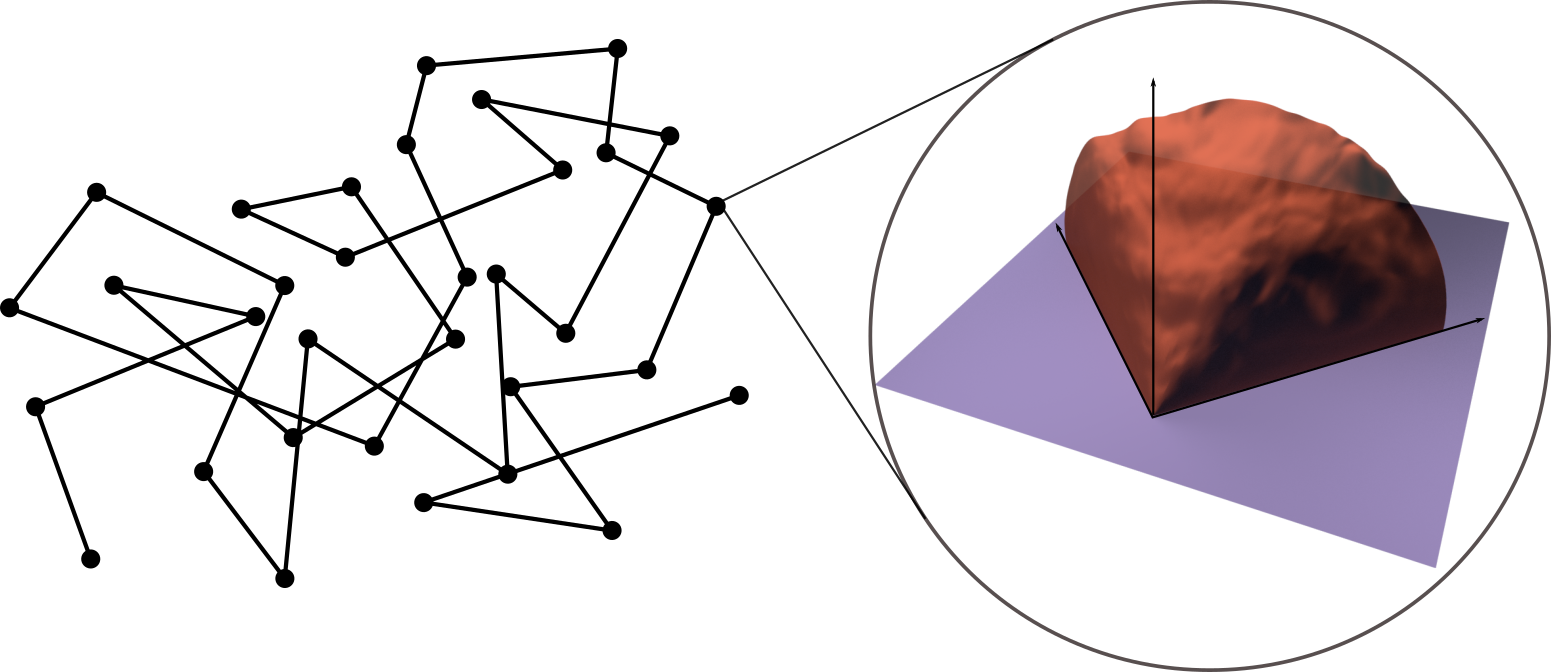
\includegraphics[width=1.3\textwidth]{markov.png}};
\begin{scope}[x={(image.south east)},y={(image.north west)}]
%\node [anchor=north] at (0.6,0.37) {$\mathcal{C}_{\rm cusp}$};
\node [anchor=south] at (0.74,0.89) {$z$};
\node [anchor=south] at (0.46,0.7) {$\phi_{i}$};
\node [anchor=east] at (0.68,0.65) {$x^{+}$};
\node [anchor=west] at (0.95,0.53) {$x^{-}$};
%\draw[help lines,xstep=.1,ystep=.1] (0,0) grid (1,1);
%\foreach \x in {0,1,...,9} { \node [anchor=north] at (\x/10,0) {0.\x}; }
%\foreach \y in {0,1,...,9} { \node [anchor=east] at (0,\y/10) {0.\y}; }
\end{scope}
\end{tikzpicture}
\end{center}
}
\end{frame}

%###############################################

\begin{frame}
\frametitle{Simulation parameters and continuum limit}
\begin{itemize}
\item Parameters in the continuum: $g$, $m$
\item Dimensionless parameters on the lattice:\\
\begin{center}
$g$, $L$ $(T\equiv 2L)$ , $M\equiv ma$
\end{center}
\item Any observable on lattice is function of input parameters\\
\begin{center}
$\langle F_{\rm LAT} \rangle = \langle F_{\rm LAT}(g,L,M) \rangle = \langle F(g) \rangle + \mathcal{O}(L^{-1}) + \mathcal{O}(e^{-LM})$
\end{center}
\item Continuum limit $\langle F(g) \rangle$ obtained via extrapolation to infinite $L$ $(a\to 0)$
\end{itemize}
\end{frame}

%##############################################

\begin{frame}
\begin{itemize}
\item Take cont. limit in controlled way - {\color{blue!90} Line of constant Physics:}
\begin{itemize}
\item Renormalised physical mass in continuum\\
\begin{center}
$m_{x}^{2}(g) = \frac{m^{2}}{2} \big(1- 1/(8g) + \mathcal{O}(g^{-2})\big)\quad {\color{red}(\ast)}$
\end{center}
\item Keep dimensionless physical quantities constant while $a\to 0$\\
\begin{center}
$\frac{V_{2}m_{x}^{2}}{2} \quad \xrightarrow{g \;{\rm fixed}}{} \quad \frac{V_{2}m^{2}}{2} = (LM)^{2} = {\rm const.}$
\end{center}
if ${\small \color{red}(\ast)}$ is also true on the lattice
\end{itemize}\vspace{2mm}
\item Procedure:
\begin{itemize}
\item Fix $g$
\item Fix $LM$ large enough to keep finite volume effects small
\item Evaluate $\langle F_{\rm LAT} \rangle$ for $L=8,10,12,16,\ldots$
\item Extrapolate to $L\to \infty$ to obtain $\langle F(g) \rangle$
\end{itemize}
\end{itemize}

\begin{center}

\begin{tikzpicture}[scale=0.7, every node/.style={scale=0.8}]
\draw (-1,-1) rectangle (1,1);
\path (-1,-1) -- node[below]{\footnotesize $L=5$} (1,-1);
\path (-1.7,-1) -- node[left]{\footnotesize $LM=c,$} (-1.7,1);
\path (-1,1) -- node[above]{\footnotesize $M=c/5$} (1,1);
\draw [step=0.5cm,dashed] (-1,-1) grid (1,1);
%\path (0,0) circle (0.6pt) node[below=2pt, fill=white]{\tiny $(an_{0},an_{1})$};
\foreach \x in {-1,-0.5,...,1}{
	\foreach \y in {-1,-0.5,...,1}{
		\fill (\x,\y) circle (0.6pt);
	}
}
\end{tikzpicture}
\hspace{6mm}
\begin{tikzpicture}[scale=0.7, every node/.style={scale=0.8}]
%flat grid
\draw (-1,-1) rectangle (1,1);
\path (-1,-1) -- node[below]{\footnotesize $L=7$} (1,-1);
\path (-1,1) -- node[above]{\footnotesize $M=c/7$} (1,1);
%\path (-1,-1) -- node[left]{$\sigma$} (-1,1);
\draw [step=0.333cm,dashed] (-1,-1) grid (1,1);
%\path (0,0) circle (0.6pt) node[below=2pt, fill=white]{\tiny $(an_{0},an_{1})$};
\foreach \x in {-1,-0.666,...,1}{
	\foreach \y in {-1,-0.666,...,1}{
		\fill (\x,\y) circle (0.6pt);
	}
}
\end{tikzpicture}
\hspace{6mm}
\begin{tikzpicture}[scale=0.7, every node/.style={scale=0.8}]
%flat grid
\draw (-1,-1) rectangle (1,1);
\path (-1,-1) -- node[below]{\footnotesize $L=9$} (1,-1);
\path (-1,1) -- node[above]{\footnotesize $M=c/9$} (1,1);
%\path (-1,-1) -- node[left]{$\sigma$} (-1,1);
\draw [step=0.25cm,dashed] (-1,-1) grid (1,1);
%\path (0,0) circle (0.6pt) node[below=2pt, fill=white]{\tiny $(an_{0},an_{1})$};
\foreach \x in {-1,-0.75,...,1}{
	\foreach \y in {-1,-0.75,...,1}{
		\fill (\x,\y) circle (0.6pt);
	}
}
\end{tikzpicture}
\end{center}
\end{frame}

%#########################################################
\Section{Results}
{\usefoottemplate{}
\begin{frame}
\frametitle{Mass of the x field}
\begin{minipage}{0.5\linewidth}
\vspace{-20mm}
Fit timeslice correlators 
\begin{align*}
\huge C_{x}(t) &= \frac{1}{L}\sum\limits_{s_{1},s_{2}} \langle x(t,s_{1})x^{*}(0,s_{2})\rangle \\
&\sim {\rm cosh}\big( (\tfrac{T}{2}-t) m_{x{\rm LAT}} \big)
\end{align*}


\hfill\\
\vspace{10mm}
Extract mass via continuum limit\\
$\frac{m_{x \rm LAT}^{2}(L,g)}{M^{2}} = \frac{m_{x}^{2}(g)}{m^{2}} + \mathcal{O}(L^{-1})$
\end{minipage}
\begin{minipage}{0.45\linewidth}
\vspace{-10mm}
% This file was created by matlab2tikz.
%
%The latest updates can be retrieved from
%  http://www.mathworks.com/matlabcentral/fileexchange/22022-matlab2tikz-matlab2tikz
%where you can also make suggestions and rate matlab2tikz.
%
\begin{tikzpicture}[thick,scale=0.4, every node/.style={scale=1.3}]

\begin{axis}[%
width=4.585in,
height=3.591in,
at={(0.769in,0.485in)},
scale only axis,
xmin=-1,
xmax=24,
xlabel style={font=\color{white!15!black}},
xlabel={$at$},
ymin=0,
ymax=0.025,
ylabel style={font=\color{white!15!black}},
ylabel={$C_x(at)$},
axis background/.style={fill=white},
axis x line*=bottom,
axis y line*=left,
legend style={legend cell align=left, align=left, draw=white!15!black}
]
\addplot [color=blue, draw=none, mark size=1.0pt, mark=*, mark options={solid, fill=blue, blue}]
 plot [error bars/.cd, y dir = both, y explicit]
 table[row sep=crcr, y error plus index=2, y error minus index=3]{%
0	0.0243260688956114	0.000508141001299536	0.000508141001299536\\
1	0.0190365611462439	0.000495256840816025	0.000495256840816025\\
2	0.0151613082921611	0.00047550688870233	0.00047550688870233\\
3	0.0120268515516549	0.000452641748717815	0.000452641748717815\\
4	0.00954649117718522	0.000437780862197653	0.000437780862197653\\
5	0.00799378320884425	0.000427874857138029	0.000427874857138029\\
6	0.00664231426579697	0.000424177616634774	0.000424177616634774\\
7	0.00570072604922918	0.000432623989008807	0.000432623989008807\\
8	0.00468960623594428	0.000438472127189161	0.000438472127189161\\
9	0.00419824652026065	0.000448589313853651	0.000448589313853651\\
10	0.00381004107536998	0.000457257954665896	0.000457257954665896\\
11	0.00331400881610101	0.000476295971796519	0.000476295971796519\\
12	0.00326691499004617	0.000486384238136538	0.000486384238136538\\
13	0.00331400881610101	0.000476295971796519	0.000476295971796519\\
14	0.00381004107536998	0.000457257954665896	0.000457257954665896\\
15	0.00419824652026065	0.000448589313853651	0.000448589313853651\\
16	0.00468960623594429	0.000438472127189161	0.000438472127189161\\
17	0.00570072604922918	0.000432623989008807	0.000432623989008807\\
18	0.00664231426579697	0.000424177616634774	0.000424177616634774\\
19	0.00799378320884425	0.000427874857138029	0.000427874857138029\\
20	0.00954649117718522	0.000437780862197653	0.000437780862197653\\
21	0.0120268515516549	0.000452641748717815	0.000452641748717815\\
22	0.0151613082921611	0.00047550688870233	0.00047550688870233\\
23	0.0190365611462439	0.000495256840816025	0.000495256840816025\\
};
\addlegendentry{Data: $L=12$ $g=100$}

\addplot [color=red]
  table[row sep=crcr]{%
1	0.018815021481251\\
2	0.015153649523578\\
3	0.0122333397946224\\
4	0.00991127975058608\\
5	0.00807391318253274\\
6	0.00663138695232729\\
7	0.00551315688501861\\
8	0.00466453793166128\\
9	0.0040440298944364\\
10	0.00362128793342356\\
11	0.00337563860627392\\
12	0.00329506887034864\\
13	0.00337563860627392\\
14	0.00362128793342356\\
15	0.0040440298944364\\
16	0.00466453793166128\\
17	0.00551315688501861\\
18	0.00663138695232729\\
19	0.00807391318253274\\
20	0.00991127975058608\\
21	0.0122333397946224\\
22	0.015153649523578\\
23	0.018815021481251\\
};
\addlegendentry{Fit to cosh}

\addplot [color=red, dashed]
  table[row sep=crcr]{%
1	0.0185686944823777\\
2	0.0147741284170975\\
3	0.0117793632850322\\
4	0.00942227676804811\\
5	0.0075752674305322\\
6	0.00613834698552117\\
7	0.00503372740515777\\
8	0.00420160984742034\\
9	0.00359694743167847\\
10	0.0031870066151649\\
11	0.0029495951549023\\
12	0.00287186072538535\\
13	0.0029495951549023\\
14	0.0031870066151649\\
15	0.00359694743167847\\
16	0.00420160984742034\\
17	0.00503372740515777\\
18	0.00613834698552117\\
19	0.0075752674305322\\
20	0.00942227676804811\\
21	0.0117793632850322\\
22	0.0147741284170975\\
23	0.0185686944823777\\
};
\addlegendentry{Fit errors}

\addplot [color=red, dashed, forget plot]
  table[row sep=crcr]{%
1	0.0190739501095884\\
2	0.0155526061974642\\
3	0.0127146450612897\\
4	0.0104353664588898\\
5	0.00861461870387236\\
6	0.00717239799241623\\
7	0.00604533302965205\\
8	0.005183900489833\\
9	0.00455024895739046\\
10	0.00411653573266837\\
11	0.00386370342144523\\
12	0.00378064255148857\\
13	0.00386370342144523\\
14	0.00411653573266837\\
15	0.00455024895739046\\
16	0.005183900489833\\
17	0.00604533302965205\\
18	0.00717239799241623\\
19	0.00861461870387236\\
20	0.0104353664588898\\
21	0.0127146450612897\\
22	0.0155526061974642\\
23	0.0190739501095884\\
};
\end{axis}
\end{tikzpicture}%\\
\vspace{-6mm}
% This file was created by matlab2tikz.
%
%The latest updates can be retrieved from
%  http://www.mathworks.com/matlabcentral/fileexchange/22022-matlab2tikz-matlab2tikz
%where you can also make suggestions and rate matlab2tikz.
%
\definecolor{mycolor1}{rgb}{0.00000,0.44700,0.74100}%
%
\begin{tikzpicture}[thick,scale=0.4, every node/.style={scale=1.3}]

\begin{axis}[%
width=4.521in,
height=3.548in,
at={(0.758in,0.499in)},
scale only axis,
xmin=0,
xmax=4.5,
xlabel style={font=\color{white!15!black}},
xlabel={$g_{\rm c}$},
ymin=0.25,
ymax=0.6,
ylabel style={font=\color{white!15!black}},
ylabel={$m_x^2/m^2$},
axis background/.style={fill=white},
axis x line*=bottom,
axis y line*=left,
legend style={legend cell align=left, align=left, draw=white!15!black}
]
\addplot [color=mycolor1, draw=none, mark=*, mark options={solid, mycolor1}]
 plot [error bars/.cd, y dir = both, y explicit]
 table[row sep=crcr, y error plus index=2, y error minus index=3]{%
0.2	0.490165571995369	0.0940854482495643	0.0940854482495643\\
0.4	0.452690842104691	0.0679665829360463	0.0679665829360463\\
0.6	0.346358687566165	0.0532360302975794	0.0532360302975794\\
0.8	0.406262875267605	0.0281024418118495	0.0281024418118495\\
1	0.469437254056113	0.0268544852814218	0.0268544852814218\\
1.2	0.445751222819117	0.0201282079389417	0.0201282079389417\\
1.6	0.446319902479861	0.0213564289850636	0.0213564289850636\\
2	0.49048642935341	0.0206704061178771	0.0206704061178771\\
2.4	0.495107471223214	0.0503207897225451	0.0503207897225451\\
2.8	0.417886014437159	0.0406259420793661	0.0406259420793661\\
4	0.347117170064447	0.0659769038512879	0.0659769038512879\\
};
\addlegendentry{$LM = 4$}

\addplot [color=black, dotted]
  table[row sep=crcr]{%
1	0.4375\\
1.03030303030303	0.439338235294118\\
1.06060606060606	0.441071428571429\\
1.09090909090909	0.442708333333333\\
1.12121212121212	0.444256756756757\\
1.15151515151515	0.445723684210526\\
1.18181818181818	0.447115384615385\\
1.21212121212121	0.4484375\\
1.24242424242424	0.44969512195122\\
1.27272727272727	0.450892857142857\\
1.3030303030303	0.45203488372093\\
1.33333333333333	0.453125\\
1.36363636363636	0.454166666666667\\
1.39393939393939	0.455163043478261\\
1.42424242424242	0.456117021276596\\
1.45454545454545	0.45703125\\
1.48484848484848	0.457908163265306\\
1.51515151515152	0.45875\\
1.54545454545455	0.459558823529412\\
1.57575757575758	0.460336538461538\\
1.60606060606061	0.461084905660377\\
1.63636363636364	0.461805555555556\\
1.66666666666667	0.4625\\
1.6969696969697	0.463169642857143\\
1.72727272727273	0.463815789473684\\
1.75757575757576	0.464439655172414\\
1.78787878787879	0.465042372881356\\
1.81818181818182	0.465625\\
1.84848484848485	0.466188524590164\\
1.87878787878788	0.466733870967742\\
1.90909090909091	0.467261904761905\\
1.93939393939394	0.4677734375\\
1.96969696969697	0.468269230769231\\
2	0.46875\\
2.03030303030303	0.469216417910448\\
2.06060606060606	0.469669117647059\\
2.09090909090909	0.470108695652174\\
2.12121212121212	0.470535714285714\\
2.15151515151515	0.470950704225352\\
2.18181818181818	0.471354166666667\\
2.21212121212121	0.471746575342466\\
2.24242424242424	0.472128378378378\\
2.27272727272727	0.4725\\
2.3030303030303	0.472861842105263\\
2.33333333333333	0.473214285714286\\
2.36363636363636	0.473557692307692\\
2.39393939393939	0.473892405063291\\
2.42424242424242	0.47421875\\
2.45454545454545	0.474537037037037\\
2.48484848484848	0.47484756097561\\
2.51515151515152	0.475150602409639\\
2.54545454545455	0.475446428571429\\
2.57575757575758	0.475735294117647\\
2.60606060606061	0.476017441860465\\
2.63636363636364	0.476293103448276\\
2.66666666666667	0.4765625\\
2.6969696969697	0.476825842696629\\
2.72727272727273	0.477083333333333\\
2.75757575757576	0.477335164835165\\
2.78787878787879	0.47758152173913\\
2.81818181818182	0.477822580645161\\
2.84848484848485	0.478058510638298\\
2.87878787878788	0.478289473684211\\
2.90909090909091	0.478515625\\
2.93939393939394	0.478737113402062\\
2.96969696969697	0.478954081632653\\
3	0.479166666666667\\
3.03030303030303	0.479375\\
3.06060606060606	0.479579207920792\\
3.09090909090909	0.479779411764706\\
3.12121212121212	0.47997572815534\\
3.15151515151515	0.480168269230769\\
3.18181818181818	0.480357142857143\\
3.21212121212121	0.480542452830189\\
3.24242424242424	0.480724299065421\\
3.27272727272727	0.480902777777778\\
3.3030303030303	0.481077981651376\\
3.33333333333333	0.48125\\
3.36363636363636	0.481418918918919\\
3.39393939393939	0.481584821428571\\
3.42424242424242	0.481747787610619\\
3.45454545454545	0.481907894736842\\
3.48484848484848	0.482065217391304\\
3.51515151515152	0.482219827586207\\
3.54545454545455	0.482371794871795\\
3.57575757575758	0.482521186440678\\
3.60606060606061	0.482668067226891\\
3.63636363636364	0.4828125\\
3.66666666666667	0.482954545454545\\
3.6969696969697	0.483094262295082\\
3.72727272727273	0.483231707317073\\
3.75757575757576	0.483366935483871\\
3.78787878787879	0.4835\\
3.81818181818182	0.483630952380952\\
3.84848484848485	0.483759842519685\\
3.87878787878788	0.48388671875\\
3.90909090909091	0.484011627906977\\
3.93939393939394	0.484134615384615\\
3.96969696969697	0.48425572519084\\
4	0.484375\\
};
\addlegendentry{PT, $g_{\rm c}=0.04 g$}

\end{axis}
\end{tikzpicture}%
\end{minipage}
\end{frame}

%########################################

\begin{frame}
\frametitle{The cusp action}
\begin{itemize}
\item Observe quadratic divergences $\langle S_{\rm cusp}^{(2)}\rangle \sim \frac{V_{2}}{2}(N_{\rm B}-N_{\rm F})$
\item On the lattice study only bosonic part of the action\\
\begin{center}
$\langle S_{\rm LAT} \rangle = g \frac{(LM)^{2}}{4}f'(g) + \frac{c(g)}{2}(2L^{2}), \quad c(g) = N_{\rm B} +\mathcal{O}(g^{-1})$
\end{center}
\end{itemize}
\vspace{4mm}
\only<1>{
\begin{minipage}{0.48\linewidth}
\begin{center}
\vspace{2mm}
\hspace{-5mm}
% This file was created by matlab2tikz.
%
%The latest updates can be retrieved from
%  http://www.mathworks.com/matlabcentral/fileexchange/22022-matlab2tikz-matlab2tikz
%where you can also make suggestions and rate matlab2tikz.
%
\definecolor{mycolor1}{rgb}{0.00000,0.44700,0.74100}%
%
\begin{tikzpicture}[thick,scale=0.4, every node/.style={scale=1.3}]

\begin{axis}[%
width=4.521in,
height=3.554in,
at={(0.758in,0.782in)},
scale only axis,
xmin=-0.00356393129770993,
xmax=0.104756679389313,
%xmax=0.21,
xtick={0,0.01,0.0166666666666667,0.025,0.0333333333333333,0.04,0.0666666666666667,0.1,0.2},
xticklabels={{0},{1/100},{1/60},{1/40},{1/30},{1/25},{1/15},{1/10},{1/5}},
xticklabel style={rotate=45},
xlabel style={font=\color{white!15!black}},
xlabel={$1/g$},
ymin=12.4625321336761,
ymax=12.5743573264782,
%ymax=12.63,
ylabel style={font=\color{white!15!black}},
ylabel={$c/2$},
axis background/.style={fill=white},
axis x line*=bottom,
axis y line*=left,
legend style={at={(0.03,0.97)}, anchor=north west, legend cell align=left, align=left, draw=white!15!black}
]
\addplot [color=mycolor1, draw=none, mark=*, mark options={solid, mycolor1}]
 plot [error bars/.cd, y dir = both, y explicit]
 table[row sep=crcr, y error plus index=2, y error minus index=3]{%
0.2	12.6224700841751	0.0035673092009017	0.0035673092009017\\
0.1	12.5333064346217	0.00191119909436733	0.00191119909436733\\
0.0666666666666667	12.5117413581589	0.00546179104759107	0.00546179104759107\\
0.05	12.5092754189257	0.00943604846448236	0.00943604846448236\\
0.04	12.4996326057472	0.00262893477657402	0.00262893477657402\\
0.0333333333333333	12.4984550678755	0.00107274344858564	0.00107274344858564\\
0.025	12.4976072932875	0.00123483678129764	0.00123483678129764\\
0.02	12.4975434224159	0.00142456884245334	0.00142456884245334\\
0.0166666666666667	12.5011509717621	0.00358437551326972	0.00358437551326972\\
0.0142857142857143	12.4938758847144	0.00526638906021808	0.00526638906021808\\
0.01	12.5064759519801	0.00514755803286955	0.00514755803286955\\
};
\addlegendentry{$LM = 4$}

\addplot [color=black, dashed]
  table[row sep=crcr]{%
0	12.5\\
0.002	12.4998723674817\\
0.004	12.4997447349634\\
0.006	12.4996171024451\\
0.008	12.4994894699267\\
0.01	12.4993618374084\\
0.012	12.4992342048901\\
0.014	12.4991065723718\\
0.016	12.4989789398535\\
0.018	12.4988513073352\\
0.02	12.4987236748168\\
0.022	12.4985960422985\\
0.024	12.4984684097802\\
0.026	12.4983407772619\\
0.028	12.4982131447436\\
0.03	12.4980855122253\\
0.032	12.4979578797069\\
0.034	12.4978302471886\\
0.036	12.4977026146703\\
0.038	12.497574982152\\
0.04	12.4974473496337\\
0.042	12.4973197171154\\
0.044	12.497192084597\\
0.046	12.4970644520787\\
0.048	12.4969368195604\\
0.05	12.4968091870421\\
0.052	12.4966815545238\\
0.054	12.4965539220055\\
0.056	12.4964262894871\\
0.058	12.4962986569688\\
0.06	12.4961710244505\\
0.062	12.4960433919322\\
0.064	12.4959157594139\\
0.066	12.4957881268956\\
0.068	12.4956604943772\\
0.07	12.4955328618589\\
0.072	12.4954052293406\\
0.074	12.4952775968223\\
0.076	12.495149964304\\
0.078	12.4950223317857\\
0.08	12.4948946992674\\
0.082	12.494767066749\\
0.084	12.4946394342307\\
0.086	12.4945118017124\\
0.088	12.4943841691941\\
0.09	12.4942565366758\\
0.092	12.4941289041575\\
0.094	12.4940012716391\\
0.096	12.4938736391208\\
0.098	12.4937460066025\\
0.1	12.4936183740842\\
0.102	12.4934907415659\\
0.104	12.4933631090476\\
0.106	12.4932354765292\\
0.108	12.4931078440109\\
0.11	12.4929802114926\\
0.112	12.4928525789743\\
0.114	12.492724946456\\
0.116	12.4925973139377\\
0.118	12.4924696814193\\
0.12	12.492342048901\\
0.122	12.4922144163827\\
0.124	12.4920867838644\\
0.126	12.4919591513461\\
0.128	12.4918315188278\\
0.13	12.4917038863094\\
0.132	12.4915762537911\\
0.134	12.4914486212728\\
0.136	12.4913209887545\\
0.138	12.4911933562362\\
0.14	12.4910657237179\\
0.142	12.4909380911995\\
0.144	12.4908104586812\\
0.146	12.4906828261629\\
0.148	12.4905551936446\\
0.15	12.4904275611263\\
0.152	12.490299928608\\
0.154	12.4901722960896\\
0.156	12.4900446635713\\
0.158	12.489917031053\\
0.16	12.4897893985347\\
0.162	12.4896617660164\\
0.164	12.4895341334981\\
0.166	12.4894065009798\\
0.168	12.4892788684614\\
0.17	12.4891512359431\\
0.172	12.4890236034248\\
0.174	12.4888959709065\\
0.176	12.4887683383882\\
0.178	12.4886407058699\\
0.18	12.4885130733515\\
0.182	12.4883854408332\\
0.184	12.4882578083149\\
0.186	12.4881301757966\\
0.188	12.4880025432783\\
0.19	12.48787491076\\
0.192	12.4877472782416\\
0.194	12.4876196457233\\
0.196	12.487492013205\\
0.198	12.4873643806867\\
0.2	12.4872367481684\\
0.202	12.4871091156501\\
0.204	12.4869814831317\\
0.206	12.4868538506134\\
0.208	12.4867262180951\\
0.21	12.4865985855768\\
};
\addlegendentry{$\text{lin. fit, } g\geq 70$}

\addplot [color=black, dotted]
  table[row sep=crcr]{%
0	12.5\\
0.002	12.4995662974101\\
0.004	12.4991775486241\\
0.006	12.4988337536418\\
0.008	12.4985349124633\\
0.01	12.4982810250886\\
0.012	12.4980720915176\\
0.014	12.4979081117504\\
0.016	12.4977890857871\\
0.018	12.4977150136274\\
0.02	12.4976858952716\\
0.022	12.4977017307196\\
0.024	12.4977625199713\\
0.026	12.4978682630268\\
0.028	12.4980189598861\\
0.03	12.4982146105492\\
0.032	12.4984552150161\\
0.034	12.4987407732867\\
0.036	12.4990712853611\\
0.038	12.4994467512393\\
0.04	12.4998671709213\\
0.042	12.5003325444071\\
0.044	12.5008428716966\\
0.046	12.5013981527899\\
0.048	12.501998387687\\
0.05	12.5026435763879\\
0.052	12.5033337188926\\
0.054	12.504068815201\\
0.056	12.5048488653133\\
0.058	12.5056738692293\\
0.06	12.506543826949\\
0.062	12.5074587384726\\
0.064	12.5084186038\\
0.066	12.5094234229311\\
0.068	12.510473195866\\
0.07	12.5115679226047\\
0.072	12.5127076031472\\
0.074	12.5138922374934\\
0.076	12.5151218256434\\
0.078	12.5163963675973\\
0.08	12.5177158633548\\
0.082	12.5190803129162\\
0.084	12.5204897162814\\
0.086	12.5219440734503\\
0.088	12.523443384423\\
0.09	12.5249876491995\\
0.092	12.5265768677798\\
0.094	12.5282110401638\\
0.096	12.5298901663517\\
0.098	12.5316142463433\\
0.1	12.5333832801387\\
0.102	12.5351972677379\\
0.104	12.5370562091408\\
0.106	12.5389601043476\\
0.108	12.5409089533581\\
0.11	12.5429027561724\\
0.112	12.5449415127905\\
0.114	12.5470252232123\\
0.116	12.549153887438\\
0.118	12.5513275054674\\
0.12	12.5535460773006\\
0.122	12.5558096029376\\
0.124	12.5581180823784\\
0.126	12.5604715156229\\
0.128	12.5628699026712\\
0.13	12.5653132435234\\
0.132	12.5678015381792\\
0.134	12.5703347866389\\
0.136	12.5729129889024\\
0.138	12.5755361449696\\
0.14	12.5782042548406\\
0.142	12.5809173185154\\
0.144	12.583675335994\\
0.146	12.5864783072763\\
0.148	12.5893262323624\\
0.15	12.5922191112524\\
0.152	12.5951569439461\\
0.154	12.5981397304435\\
0.156	12.6011674707448\\
0.158	12.6042401648498\\
0.16	12.6073578127586\\
0.162	12.6105204144712\\
0.164	12.6137279699876\\
0.166	12.6169804793078\\
0.168	12.6202779424317\\
0.17	12.6236203593594\\
0.172	12.6270077300909\\
0.174	12.6304400546262\\
0.176	12.6339173329653\\
0.178	12.6374395651081\\
0.18	12.6410067510547\\
0.182	12.6446188908051\\
0.184	12.6482759843593\\
0.186	12.6519780317173\\
0.188	12.655725032879\\
0.19	12.6595169878445\\
0.192	12.6633538966139\\
0.194	12.6672357591869\\
0.196	12.6711625755638\\
0.198	12.6751343457444\\
0.2	12.6791510697289\\
0.202	12.6832127475171\\
0.204	12.6873193791091\\
0.206	12.6914709645048\\
0.208	12.6956675037044\\
0.21	12.6999089967077\\
};
\addlegendentry{$\text{quad. fit, } g\geq 10$}

\end{axis}
\end{tikzpicture}%
\end{center}
\end{minipage}
\begin{minipage}{0.48\linewidth}
\begin{center}
% This file was created by matlab2tikz.
%
%The latest updates can be retrieved from
%  http://www.mathworks.com/matlabcentral/fileexchange/22022-matlab2tikz-matlab2tikz
%where you can also make suggestions and rate matlab2tikz.
%
\definecolor{mycolor1}{rgb}{0.00000,0.44700,0.74100}%
\definecolor{mycolor2}{rgb}{0.85000,0.32500,0.09800}%
\definecolor{mycolor3}{rgb}{0.92900,0.69400,0.12500}%
\definecolor{mycolor4}{rgb}{0.49400,0.18400,0.55600}%
\definecolor{mycolor5}{rgb}{0.46600,0.67400,0.18800}%
\definecolor{mycolor6}{rgb}{0.63500,0.07800,0.18400}%
\definecolor{mycolor7}{rgb}{0.30100,0.74500,0.93300}%
%
\begin{tikzpicture}[thick,scale=0.42, every node/.style={scale=1.3}]

\begin{axis}[%
width=4.521in,
height=3.566in,
at={(0.758in,0.481in)},
scale only axis,
xmin=-0.005,
xmax=0.17,
xlabel style={font=\color{white!15!black}},
xlabel={$1/L$},
xtick={0,0.02,0.04,0.06,0.08,0.1,0.12,0.14,0.16},
xticklabels={{0},{0.02},{0.04},{0.06},{0.08},{0.1},{0.12},{0.14},{0.16}},
ymin=1.5,
ymax=6.5,
ylabel style={font=\color{white!15!black}},
ylabel={$(\langle S_{\rm LAT} \rangle - c/2 (2L^2)) / S_0 + \ln(g)$},
axis background/.style={fill=white},
axis x line*=bottom,
axis y line*=left
]
\addplot [color=mycolor1, dotted, forget plot]
  table[row sep=crcr]{%
0	2.43727316330578\\
0.00125	2.43727316330578\\
0.0025	2.43727316330578\\
0.00375	2.43727316330578\\
0.005	2.43727316330578\\
0.00625	2.43727316330578\\
0.0075	2.43727316330578\\
0.00875	2.43727316330578\\
0.01	2.43727316330578\\
0.01125	2.43727316330578\\
0.0125	2.43727316330578\\
0.01375	2.43727316330578\\
0.015	2.43727316330578\\
0.01625	2.43727316330578\\
0.0175	2.43727316330578\\
0.01875	2.43727316330578\\
0.02	2.43727316330578\\
0.02125	2.43727316330578\\
0.0225	2.43727316330578\\
0.02375	2.43727316330578\\
0.025	2.43727316330578\\
0.02625	2.43727316330578\\
0.0275	2.43727316330578\\
0.02875	2.43727316330578\\
0.03	2.43727316330578\\
0.03125	2.43727316330578\\
0.0325	2.43727316330578\\
0.03375	2.43727316330578\\
0.035	2.43727316330578\\
0.03625	2.43727316330578\\
0.0375	2.43727316330578\\
0.03875	2.43727316330578\\
0.04	2.43727316330578\\
0.04125	2.43727316330578\\
0.0425	2.43727316330578\\
0.04375	2.43727316330578\\
0.045	2.43727316330578\\
0.04625	2.43727316330578\\
0.0475	2.43727316330578\\
0.04875	2.43727316330578\\
0.05	2.43727316330578\\
0.05125	2.43727316330578\\
0.0525	2.43727316330578\\
0.05375	2.43727316330578\\
0.055	2.43727316330578\\
0.05625	2.43727316330578\\
0.0575	2.43727316330578\\
0.05875	2.43727316330578\\
0.06	2.43727316330578\\
0.06125	2.43727316330578\\
0.0625	2.43727316330578\\
0.06375	2.43727316330578\\
0.065	2.43727316330578\\
0.06625	2.43727316330578\\
0.0675	2.43727316330578\\
0.06875	2.43727316330578\\
0.07	2.43727316330578\\
0.07125	2.43727316330578\\
0.0725	2.43727316330578\\
0.07375	2.43727316330578\\
0.075	2.43727316330578\\
0.07625	2.43727316330578\\
0.0775	2.43727316330578\\
0.07875	2.43727316330578\\
0.08	2.43727316330578\\
0.08125	2.43727316330578\\
0.0825	2.43727316330578\\
};
\addplot [color=mycolor1, dashed, forget plot]
  table[row sep=crcr]{%
0	2.43328517943851\\
0.00125	2.43336689492752\\
0.0025	2.43344861041653\\
0.00375	2.43353032590553\\
0.005	2.43361204139454\\
0.00625	2.43369375688355\\
0.0075	2.43377547237255\\
0.00875	2.43385718786156\\
0.01	2.43393890335056\\
0.01125	2.43402061883957\\
0.0125	2.43410233432858\\
0.01375	2.43418404981758\\
0.015	2.43426576530659\\
0.01625	2.4343474807956\\
0.0175	2.4344291962846\\
0.01875	2.43451091177361\\
0.02	2.43459262726261\\
0.02125	2.43467434275162\\
0.0225	2.43475605824063\\
0.02375	2.43483777372963\\
0.025	2.43491948921864\\
0.02625	2.43500120470765\\
0.0275	2.43508292019665\\
0.02875	2.43516463568566\\
0.03	2.43524635117466\\
0.03125	2.43532806666367\\
0.0325	2.43540978215268\\
0.03375	2.43549149764168\\
0.035	2.43557321313069\\
0.03625	2.4356549286197\\
0.0375	2.4357366441087\\
0.03875	2.43581835959771\\
0.04	2.43590007508672\\
0.04125	2.43598179057572\\
0.0425	2.43606350606473\\
0.04375	2.43614522155373\\
0.045	2.43622693704274\\
0.04625	2.43630865253175\\
0.0475	2.43639036802075\\
0.04875	2.43647208350976\\
0.05	2.43655379899877\\
0.05125	2.43663551448777\\
0.0525	2.43671722997678\\
0.05375	2.43679894546578\\
0.055	2.43688066095479\\
0.05625	2.4369623764438\\
0.0575	2.4370440919328\\
0.05875	2.43712580742181\\
0.06	2.43720752291082\\
0.06125	2.43728923839982\\
0.0625	2.43737095388883\\
0.06375	2.43745266937784\\
0.065	2.43753438486684\\
0.06625	2.43761610035585\\
0.0675	2.43769781584485\\
0.06875	2.43777953133386\\
0.07	2.43786124682287\\
0.07125	2.43794296231187\\
0.0725	2.43802467780088\\
0.07375	2.43810639328989\\
0.075	2.43818810877889\\
0.07625	2.4382698242679\\
0.0775	2.4383515397569\\
0.07875	2.43843325524591\\
0.08	2.43851497073492\\
0.08125	2.43859668622392\\
0.0825	2.43867840171293\\
0.08375	2.43876011720194\\
0.085	2.43884183269094\\
0.08625	2.43892354817995\\
0.0875	2.43900526366895\\
0.08875	2.43908697915796\\
0.09	2.43916869464697\\
0.09125	2.43925041013597\\
0.0925	2.43933212562498\\
0.09375	2.43941384111399\\
0.095	2.43949555660299\\
0.09625	2.439577272092\\
0.0975	2.43965898758101\\
0.09875	2.43974070307001\\
0.1	2.43982241855902\\
0.10125	2.43990413404802\\
0.1025	2.43998584953703\\
0.10375	2.44006756502604\\
0.105	2.44014928051504\\
0.10625	2.44023099600405\\
0.1075	2.44031271149306\\
0.10875	2.44039442698206\\
0.11	2.44047614247107\\
0.11125	2.44055785796008\\
0.1125	2.44063957344908\\
0.11375	2.44072128893809\\
0.115	2.44080300442709\\
0.11625	2.4408847199161\\
0.1175	2.44096643540511\\
0.11875	2.44104815089411\\
0.12	2.44112986638312\\
0.12125	2.44121158187213\\
0.1225	2.44129329736113\\
0.12375	2.44137501285014\\
0.125	2.44145672833914\\
};
\addplot [color=mycolor1, draw=none, mark=square, mark options={solid, mycolor1}, forget plot]
 plot [error bars/.cd, y dir = both, y explicit]
 table[row sep=crcr, y error plus index=2, y error minus index=3]{%
0	2.43328517943851	0.0571160600925337	0.0571160600925337\\
-0.0025	2.43727316330578	0.0206422459243649	0.0206422459243649\\
0.125	2.44193553690936	0.0138049762723457	0.0138049762723457\\
0.0833333333333333	2.43423636264366	0.0244248639926938	0.0244248639926938\\
0.0625	2.44486379605648	0.0386156190398151	0.0386156190398151\\
};
\node[right, align=left]
at (axis cs:0.126,2.542) {$g = 5$};
\addplot [color=mycolor2, dotted, forget plot]
  table[row sep=crcr]{%
0	3.24982928552263\\
0.00125	3.24982928552263\\
0.0025	3.24982928552263\\
0.00375	3.24982928552263\\
0.005	3.24982928552263\\
0.00625	3.24982928552263\\
0.0075	3.24982928552263\\
0.00875	3.24982928552263\\
0.01	3.24982928552263\\
0.01125	3.24982928552263\\
0.0125	3.24982928552263\\
0.01375	3.24982928552263\\
0.015	3.24982928552263\\
0.01625	3.24982928552263\\
0.0175	3.24982928552263\\
0.01875	3.24982928552263\\
0.02	3.24982928552263\\
0.02125	3.24982928552263\\
0.0225	3.24982928552263\\
0.02375	3.24982928552263\\
0.025	3.24982928552263\\
0.02625	3.24982928552263\\
0.0275	3.24982928552263\\
0.02875	3.24982928552263\\
0.03	3.24982928552263\\
0.03125	3.24982928552263\\
0.0325	3.24982928552263\\
0.03375	3.24982928552263\\
0.035	3.24982928552263\\
0.03625	3.24982928552263\\
0.0375	3.24982928552263\\
0.03875	3.24982928552263\\
0.04	3.24982928552263\\
0.04125	3.24982928552263\\
};
\addplot [color=mycolor2, dashed, forget plot]
  table[row sep=crcr]{%
0	3.21703525642333\\
0.00125	3.21727601730145\\
0.0025	3.21751677817957\\
0.00375	3.21775753905768\\
0.005	3.2179982999358\\
0.00625	3.21823906081392\\
0.0075	3.21847982169204\\
0.00875	3.21872058257015\\
0.01	3.21896134344827\\
0.01125	3.21920210432639\\
0.0125	3.21944286520451\\
0.01375	3.21968362608263\\
0.015	3.21992438696074\\
0.01625	3.22016514783886\\
0.0175	3.22040590871698\\
0.01875	3.2206466695951\\
0.02	3.22088743047321\\
0.02125	3.22112819135133\\
0.0225	3.22136895222945\\
0.02375	3.22160971310757\\
0.025	3.22185047398568\\
0.02625	3.2220912348638\\
0.0275	3.22233199574192\\
0.02875	3.22257275662004\\
0.03	3.22281351749815\\
0.03125	3.22305427837627\\
0.0325	3.22329503925439\\
0.03375	3.22353580013251\\
0.035	3.22377656101063\\
0.03625	3.22401732188874\\
0.0375	3.22425808276686\\
0.03875	3.22449884364498\\
0.04	3.2247396045231\\
0.04125	3.22498036540121\\
0.0425	3.22522112627933\\
0.04375	3.22546188715745\\
0.045	3.22570264803557\\
0.04625	3.22594340891368\\
0.0475	3.2261841697918\\
0.04875	3.22642493066992\\
0.05	3.22666569154804\\
0.05125	3.22690645242615\\
0.0525	3.22714721330427\\
0.05375	3.22738797418239\\
0.055	3.22762873506051\\
0.05625	3.22786949593862\\
0.0575	3.22811025681674\\
0.05875	3.22835101769486\\
0.06	3.22859177857298\\
0.06125	3.2288325394511\\
0.0625	3.22907330032921\\
0.06375	3.22931406120733\\
0.065	3.22955482208545\\
0.06625	3.22979558296357\\
0.0675	3.23003634384168\\
0.06875	3.2302771047198\\
0.07	3.23051786559792\\
0.07125	3.23075862647604\\
0.0725	3.23099938735415\\
0.07375	3.23124014823227\\
0.075	3.23148090911039\\
0.07625	3.23172166998851\\
0.0775	3.23196243086662\\
0.07875	3.23220319174474\\
0.08	3.23244395262286\\
0.08125	3.23268471350098\\
0.0825	3.23292547437909\\
0.08375	3.23316623525721\\
0.085	3.23340699613533\\
0.08625	3.23364775701345\\
0.0875	3.23388851789157\\
0.08875	3.23412927876968\\
0.09	3.2343700396478\\
0.09125	3.23461080052592\\
0.0925	3.23485156140404\\
0.09375	3.23509232228215\\
0.095	3.23533308316027\\
0.09625	3.23557384403839\\
0.0975	3.23581460491651\\
0.09875	3.23605536579462\\
0.1	3.23629612667274\\
0.10125	3.23653688755086\\
0.1025	3.23677764842898\\
0.10375	3.23701840930709\\
0.105	3.23725917018521\\
0.10625	3.23749993106333\\
0.1075	3.23774069194145\\
0.10875	3.23798145281957\\
0.11	3.23822221369768\\
0.11125	3.2384629745758\\
0.1125	3.23870373545392\\
0.11375	3.23894449633204\\
0.115	3.23918525721015\\
0.11625	3.23942601808827\\
0.1175	3.23966677896639\\
0.11875	3.23990753984451\\
0.12	3.24014830072262\\
0.12125	3.24038906160074\\
0.1225	3.24062982247886\\
0.12375	3.24087058335698\\
0.125	3.24111134423509\\
};
\addplot [color=mycolor2, draw=none, mark=diamond, mark options={solid, mycolor2}, forget plot]
 plot [error bars/.cd, y dir = both, y explicit]
 table[row sep=crcr, y error plus index=2, y error minus index=3]{%
0	3.21703525642333	0.0211018662927336	0.0211018662927336\\
-0.0025	3.24982928552263	0.0269603977359257	0.0269603977359257\\
0.125	3.24400782104094	0.00672638612937152	0.00672638612937152\\
0.1	3.23068801464209	0.00958941066440683	0.00958941066440683\\
0.0833333333333333	3.22624553594453	0.0120814030249214	0.0120814030249214\\
0.0625	3.23128175759823	0.015513686533806	0.015513686533806\\
0.0416666666666667	3.2555650420081	0.0303394947622117	0.0303394947622117\\
0.03125	3.22829706468785	0.0587837658204836	0.0587837658204836\\
};
\node[right, align=left]
at (axis cs:0.126,3.344) {$g = 10$};
\addplot [color=mycolor3, dotted, forget plot]
  table[row sep=crcr]{%
0	3.68443945181043\\
0.00125	3.68443945181043\\
0.0025	3.68443945181043\\
0.00375	3.68443945181043\\
0.005	3.68443945181043\\
0.00625	3.68443945181043\\
0.0075	3.68443945181043\\
0.00875	3.68443945181043\\
0.01	3.68443945181043\\
0.01125	3.68443945181043\\
0.0125	3.68443945181043\\
0.01375	3.68443945181043\\
0.015	3.68443945181043\\
0.01625	3.68443945181043\\
0.0175	3.68443945181043\\
0.01875	3.68443945181043\\
0.02	3.68443945181043\\
0.02125	3.68443945181043\\
0.0225	3.68443945181043\\
0.02375	3.68443945181043\\
0.025	3.68443945181043\\
0.02625	3.68443945181043\\
0.0275	3.68443945181043\\
0.02875	3.68443945181043\\
0.03	3.68443945181043\\
0.03125	3.68443945181043\\
0.0325	3.68443945181043\\
0.03375	3.68443945181043\\
0.035	3.68443945181043\\
0.03625	3.68443945181043\\
0.0375	3.68443945181043\\
0.03875	3.68443945181043\\
0.04	3.68443945181043\\
0.04125	3.68443945181043\\
0.0425	3.68443945181043\\
0.04375	3.68443945181043\\
0.045	3.68443945181043\\
0.04625	3.68443945181043\\
0.0475	3.68443945181043\\
0.04875	3.68443945181043\\
0.05	3.68443945181043\\
0.05125	3.68443945181043\\
0.0525	3.68443945181043\\
0.05375	3.68443945181043\\
0.055	3.68443945181043\\
0.05625	3.68443945181043\\
0.0575	3.68443945181043\\
0.05875	3.68443945181043\\
0.06	3.68443945181043\\
0.06125	3.68443945181043\\
0.0625	3.68443945181043\\
};
\addplot [color=mycolor3, dashed, forget plot]
  table[row sep=crcr]{%
0	3.67668014355213\\
0.00125	3.67667918280858\\
0.0025	3.67667822206503\\
0.00375	3.67667726132148\\
0.005	3.67667630057794\\
0.00625	3.67667533983439\\
0.0075	3.67667437909084\\
0.00875	3.67667341834729\\
0.01	3.67667245760374\\
0.01125	3.67667149686019\\
0.0125	3.67667053611664\\
0.01375	3.67666957537309\\
0.015	3.67666861462954\\
0.01625	3.67666765388599\\
0.0175	3.67666669314244\\
0.01875	3.67666573239889\\
0.02	3.67666477165534\\
0.02125	3.67666381091179\\
0.0225	3.67666285016824\\
0.02375	3.67666188942469\\
0.025	3.67666092868115\\
0.02625	3.6766599679376\\
0.0275	3.67665900719405\\
0.02875	3.6766580464505\\
0.03	3.67665708570695\\
0.03125	3.6766561249634\\
0.0325	3.67665516421985\\
0.03375	3.6766542034763\\
0.035	3.67665324273275\\
0.03625	3.6766522819892\\
0.0375	3.67665132124565\\
0.03875	3.6766503605021\\
0.04	3.67664939975855\\
0.04125	3.676648439015\\
0.0425	3.67664747827145\\
0.04375	3.67664651752791\\
0.045	3.67664555678436\\
0.04625	3.67664459604081\\
0.0475	3.67664363529726\\
0.04875	3.67664267455371\\
0.05	3.67664171381016\\
0.05125	3.67664075306661\\
0.0525	3.67663979232306\\
0.05375	3.67663883157951\\
0.055	3.67663787083596\\
0.05625	3.67663691009241\\
0.0575	3.67663594934886\\
0.05875	3.67663498860531\\
0.06	3.67663402786176\\
0.06125	3.67663306711821\\
0.0625	3.67663210637467\\
0.06375	3.67663114563112\\
0.065	3.67663018488757\\
0.06625	3.67662922414402\\
0.0675	3.67662826340047\\
0.06875	3.67662730265692\\
0.07	3.67662634191337\\
0.07125	3.67662538116982\\
0.0725	3.67662442042627\\
0.07375	3.67662345968272\\
0.075	3.67662249893917\\
0.07625	3.67662153819562\\
0.0775	3.67662057745207\\
0.07875	3.67661961670852\\
0.08	3.67661865596497\\
0.08125	3.67661769522143\\
0.0825	3.67661673447788\\
0.08375	3.67661577373433\\
0.085	3.67661481299078\\
0.08625	3.67661385224723\\
0.0875	3.67661289150368\\
0.08875	3.67661193076013\\
0.09	3.67661097001658\\
0.09125	3.67661000927303\\
0.0925	3.67660904852948\\
0.09375	3.67660808778593\\
0.095	3.67660712704238\\
0.09625	3.67660616629883\\
0.0975	3.67660520555528\\
0.09875	3.67660424481173\\
0.1	3.67660328406819\\
0.10125	3.67660232332464\\
0.1025	3.67660136258109\\
0.10375	3.67660040183754\\
0.105	3.67659944109399\\
0.10625	3.67659848035044\\
0.1075	3.67659751960689\\
0.10875	3.67659655886334\\
0.11	3.67659559811979\\
0.11125	3.67659463737624\\
0.1125	3.67659367663269\\
0.11375	3.67659271588914\\
0.115	3.67659175514559\\
0.11625	3.67659079440204\\
0.1175	3.67658983365849\\
0.11875	3.67658887291495\\
0.12	3.6765879121714\\
0.12125	3.67658695142785\\
0.1225	3.6765859906843\\
0.12375	3.67658502994075\\
0.125	3.6765840691972\\
};
\addplot [color=mycolor3, draw=none, mark=o, mark options={solid, mycolor3}, forget plot]
 plot [error bars/.cd, y dir = both, y explicit]
 table[row sep=crcr, y error plus index=2, y error minus index=3]{%
0	3.67668014355213	0.0298127620723799	0.0298127620723799\\
-0.0025	3.68443945181043	0.0213018362804732	0.0213018362804732\\
0.125	3.67824291574353	0.00801266770548511	0.00801266770548511\\
0.1	3.66965226342043	0.0109535770188441	0.0109535770188441\\
0.0833333333333333	3.67954102817819	0.0140127715417011	0.0140127715417011\\
0.0625	3.69184839629971	0.0228771006651215	0.0228771006651215\\
0.0416666666666667	3.63613115673994	0.0584162491507788	0.0584162491507788\\
};
\node[right, align=left]
at (axis cs:0.126,3.778) {$g = 15$};
\addplot [color=mycolor4, dotted, forget plot]
  table[row sep=crcr]{%
0	3.94321711284596\\
0.00125	3.94321711284596\\
0.0025	3.94321711284596\\
0.00375	3.94321711284596\\
0.005	3.94321711284596\\
0.00625	3.94321711284596\\
0.0075	3.94321711284596\\
0.00875	3.94321711284596\\
0.01	3.94321711284596\\
0.01125	3.94321711284596\\
0.0125	3.94321711284596\\
0.01375	3.94321711284596\\
0.015	3.94321711284596\\
0.01625	3.94321711284596\\
0.0175	3.94321711284596\\
0.01875	3.94321711284596\\
0.02	3.94321711284596\\
0.02125	3.94321711284596\\
0.0225	3.94321711284596\\
0.02375	3.94321711284596\\
0.025	3.94321711284596\\
0.02625	3.94321711284596\\
0.0275	3.94321711284596\\
0.02875	3.94321711284596\\
0.03	3.94321711284596\\
0.03125	3.94321711284596\\
0.0325	3.94321711284596\\
0.03375	3.94321711284596\\
0.035	3.94321711284596\\
0.03625	3.94321711284596\\
0.0375	3.94321711284596\\
0.03875	3.94321711284596\\
0.04	3.94321711284596\\
0.04125	3.94321711284596\\
};
\addplot [color=mycolor4, dashed, forget plot]
  table[row sep=crcr]{%
0	3.97550737751373\\
0.00125	3.975240446593\\
0.0025	3.97497351567227\\
0.00375	3.97470658475154\\
0.005	3.97443965383081\\
0.00625	3.97417272291008\\
0.0075	3.97390579198935\\
0.00875	3.97363886106862\\
0.01	3.97337193014789\\
0.01125	3.97310499922716\\
0.0125	3.97283806830643\\
0.01375	3.9725711373857\\
0.015	3.97230420646497\\
0.01625	3.97203727554424\\
0.0175	3.97177034462351\\
0.01875	3.97150341370278\\
0.02	3.97123648278205\\
0.02125	3.97096955186132\\
0.0225	3.97070262094059\\
0.02375	3.97043569001986\\
0.025	3.97016875909913\\
0.02625	3.9699018281784\\
0.0275	3.96963489725767\\
0.02875	3.96936796633694\\
0.03	3.96910103541621\\
0.03125	3.96883410449548\\
0.0325	3.96856717357475\\
0.03375	3.96830024265402\\
0.035	3.96803331173329\\
0.03625	3.96776638081256\\
0.0375	3.96749944989183\\
0.03875	3.9672325189711\\
0.04	3.96696558805036\\
0.04125	3.96669865712963\\
0.0425	3.9664317262089\\
0.04375	3.96616479528817\\
0.045	3.96589786436744\\
0.04625	3.96563093344671\\
0.0475	3.96536400252598\\
0.04875	3.96509707160525\\
0.05	3.96483014068452\\
0.05125	3.96456320976379\\
0.0525	3.96429627884306\\
0.05375	3.96402934792233\\
0.055	3.9637624170016\\
0.05625	3.96349548608087\\
0.0575	3.96322855516014\\
0.05875	3.96296162423941\\
0.06	3.96269469331868\\
0.06125	3.96242776239795\\
0.0625	3.96216083147722\\
0.06375	3.96189390055649\\
0.065	3.96162696963576\\
0.06625	3.96136003871503\\
0.0675	3.9610931077943\\
0.06875	3.96082617687357\\
0.07	3.96055924595284\\
0.07125	3.96029231503211\\
0.0725	3.96002538411138\\
0.07375	3.95975845319065\\
0.075	3.95949152226992\\
0.07625	3.95922459134919\\
0.0775	3.95895766042846\\
0.07875	3.95869072950773\\
0.08	3.958423798587\\
0.08125	3.95815686766626\\
0.0825	3.95788993674553\\
0.08375	3.9576230058248\\
0.085	3.95735607490407\\
0.08625	3.95708914398334\\
0.0875	3.95682221306261\\
0.08875	3.95655528214188\\
0.09	3.95628835122115\\
0.09125	3.95602142030042\\
0.0925	3.95575448937969\\
0.09375	3.95548755845896\\
0.095	3.95522062753823\\
0.09625	3.9549536966175\\
0.0975	3.95468676569677\\
0.09875	3.95441983477604\\
0.1	3.95415290385531\\
0.10125	3.95388597293458\\
0.1025	3.95361904201385\\
0.10375	3.95335211109312\\
0.105	3.95308518017239\\
0.10625	3.95281824925166\\
0.1075	3.95255131833093\\
0.10875	3.9522843874102\\
0.11	3.95201745648947\\
0.11125	3.95175052556874\\
0.1125	3.95148359464801\\
0.11375	3.95121666372728\\
0.115	3.95094973280655\\
0.11625	3.95068280188582\\
0.1175	3.95041587096509\\
0.11875	3.95014894004436\\
0.12	3.94988200912363\\
0.12125	3.9496150782029\\
0.1225	3.94934814728216\\
0.12375	3.94908121636143\\
0.125	3.9488142854407\\
};
\addplot [color=mycolor4, draw=none, mark=triangle, mark options={solid, rotate=180, mycolor4}, forget plot]
 plot [error bars/.cd, y dir = both, y explicit]
 table[row sep=crcr, y error plus index=2, y error minus index=3]{%
0	3.97550737751373	0.0402815193782696	0.0402815193782696\\
-0.0025	3.94321711284596	0.0714662201770275	0.0714662201770275\\
0.125	3.94312481223356	0.0114429057134635	0.0114429057134635\\
0.1	3.9750566795153	0.0159777574703331	0.0159777574703331\\
0.0833333333333333	3.94974064672045	0.0184206964508344	0.0184206964508344\\
0.0625	3.95206028218883	0.0313006242966464	0.0313006242966464\\
0.0416666666666667	3.96095081576279	0.0759905395348056	0.0759905395348056\\
0.03125	3.80745358470859	0.210257439592266	0.210257439592266\\
};
\node[right, align=left]
at (axis cs:0.126,4.043) {$g = 20$};
\addplot [color=mycolor5, dotted, forget plot]
  table[row sep=crcr]{%
0	4.21484914832195\\
0.00125	4.21484914832195\\
0.0025	4.21484914832195\\
0.00375	4.21484914832195\\
0.005	4.21484914832195\\
0.00625	4.21484914832195\\
0.0075	4.21484914832195\\
0.00875	4.21484914832195\\
0.01	4.21484914832195\\
0.01125	4.21484914832195\\
0.0125	4.21484914832195\\
0.01375	4.21484914832195\\
0.015	4.21484914832195\\
0.01625	4.21484914832195\\
0.0175	4.21484914832195\\
0.01875	4.21484914832195\\
0.02	4.21484914832195\\
0.02125	4.21484914832195\\
0.0225	4.21484914832195\\
0.02375	4.21484914832195\\
0.025	4.21484914832195\\
0.02625	4.21484914832195\\
0.0275	4.21484914832195\\
0.02875	4.21484914832195\\
0.03	4.21484914832195\\
0.03125	4.21484914832195\\
0.0325	4.21484914832195\\
0.03375	4.21484914832195\\
0.035	4.21484914832195\\
0.03625	4.21484914832195\\
0.0375	4.21484914832195\\
0.03875	4.21484914832195\\
0.04	4.21484914832195\\
0.04125	4.21484914832195\\
};
\addplot [color=mycolor5, dashed, forget plot]
  table[row sep=crcr]{%
0	4.20140477798615\\
0.00125	4.20145573462367\\
0.0025	4.2015066912612\\
0.00375	4.20155764789873\\
0.005	4.20160860453626\\
0.00625	4.20165956117379\\
0.0075	4.20171051781131\\
0.00875	4.20176147444884\\
0.01	4.20181243108637\\
0.01125	4.2018633877239\\
0.0125	4.20191434436143\\
0.01375	4.20196530099895\\
0.015	4.20201625763648\\
0.01625	4.20206721427401\\
0.0175	4.20211817091154\\
0.01875	4.20216912754906\\
0.02	4.20222008418659\\
0.02125	4.20227104082412\\
0.0225	4.20232199746165\\
0.02375	4.20237295409918\\
0.025	4.2024239107367\\
0.02625	4.20247486737423\\
0.0275	4.20252582401176\\
0.02875	4.20257678064929\\
0.03	4.20262773728682\\
0.03125	4.20267869392434\\
0.0325	4.20272965056187\\
0.03375	4.2027806071994\\
0.035	4.20283156383693\\
0.03625	4.20288252047445\\
0.0375	4.20293347711198\\
0.03875	4.20298443374951\\
0.04	4.20303539038704\\
0.04125	4.20308634702457\\
0.0425	4.20313730366209\\
0.04375	4.20318826029962\\
0.045	4.20323921693715\\
0.04625	4.20329017357468\\
0.0475	4.20334113021221\\
0.04875	4.20339208684973\\
0.05	4.20344304348726\\
0.05125	4.20349400012479\\
0.0525	4.20354495676232\\
0.05375	4.20359591339985\\
0.055	4.20364687003737\\
0.05625	4.2036978266749\\
0.0575	4.20374878331243\\
0.05875	4.20379973994996\\
0.06	4.20385069658748\\
0.06125	4.20390165322501\\
0.0625	4.20395260986254\\
0.06375	4.20400356650007\\
0.065	4.2040545231376\\
0.06625	4.20410547977512\\
0.0675	4.20415643641265\\
0.06875	4.20420739305018\\
0.07	4.20425834968771\\
0.07125	4.20430930632524\\
0.0725	4.20436026296276\\
0.07375	4.20441121960029\\
0.075	4.20446217623782\\
0.07625	4.20451313287535\\
0.0775	4.20456408951288\\
0.07875	4.2046150461504\\
0.08	4.20466600278793\\
0.08125	4.20471695942546\\
0.0825	4.20476791606299\\
0.08375	4.20481887270051\\
0.085	4.20486982933804\\
0.08625	4.20492078597557\\
0.0875	4.2049717426131\\
0.08875	4.20502269925063\\
0.09	4.20507365588815\\
0.09125	4.20512461252568\\
0.0925	4.20517556916321\\
0.09375	4.20522652580074\\
0.095	4.20527748243827\\
0.09625	4.20532843907579\\
0.0975	4.20537939571332\\
0.09875	4.20543035235085\\
0.1	4.20548130898838\\
0.10125	4.20553226562591\\
0.1025	4.20558322226343\\
0.10375	4.20563417890096\\
0.105	4.20568513553849\\
0.10625	4.20573609217602\\
0.1075	4.20578704881355\\
0.10875	4.20583800545107\\
0.11	4.2058889620886\\
0.11125	4.20593991872613\\
0.1125	4.20599087536366\\
0.11375	4.20604183200119\\
0.115	4.20609278863871\\
0.11625	4.20614374527624\\
0.1175	4.20619470191377\\
0.11875	4.2062456585513\\
0.12	4.20629661518882\\
0.12125	4.20634757182635\\
0.1225	4.20639852846388\\
0.12375	4.20644948510141\\
0.125	4.20650044173894\\
};
\addplot [color=mycolor5, draw=none, mark=triangle, mark options={solid, mycolor5}, forget plot]
 plot [error bars/.cd, y dir = both, y explicit]
 table[row sep=crcr, y error plus index=2, y error minus index=3]{%
0	4.20140477798615	0.0088567602625571	0.0088567602625571\\
-0.0025	4.21484914832195	0.0165352187648858	0.0165352187648858\\
0.125	4.20650421676597	0.00243825407478115	0.00243825407478115\\
0.1	4.20719230419459	0.00334799257063447	0.00334799257063447\\
0.0833333333333333	4.20044026889185	0.00427565906460794	0.00427565906460794\\
0.0625	4.20581322077159	0.00663986958005985	0.00663986958005985\\
0.0416666666666667	4.21910681835235	0.0173525528281516	0.0173525528281516\\
0.03125	4.17282012667966	0.0545195189538031	0.0545195189538031\\
};
\node[right, align=left]
at (axis cs:0.126,4.307) {$g = 25$};
\addplot [color=mycolor6, dotted, forget plot]
  table[row sep=crcr]{%
0	4.39176690611519\\
0.00125	4.39176690611519\\
0.0025	4.39176690611519\\
0.00375	4.39176690611519\\
0.005	4.39176690611519\\
0.00625	4.39176690611519\\
0.0075	4.39176690611519\\
0.00875	4.39176690611519\\
0.01	4.39176690611519\\
0.01125	4.39176690611519\\
0.0125	4.39176690611519\\
0.01375	4.39176690611519\\
0.015	4.39176690611519\\
0.01625	4.39176690611519\\
0.0175	4.39176690611519\\
0.01875	4.39176690611519\\
0.02	4.39176690611519\\
0.02125	4.39176690611519\\
0.0225	4.39176690611519\\
0.02375	4.39176690611519\\
0.025	4.39176690611519\\
0.02625	4.39176690611519\\
0.0275	4.39176690611519\\
0.02875	4.39176690611519\\
0.03	4.39176690611519\\
0.03125	4.39176690611519\\
0.0325	4.39176690611519\\
0.03375	4.39176690611519\\
0.035	4.39176690611519\\
0.03625	4.39176690611519\\
0.0375	4.39176690611519\\
0.03875	4.39176690611519\\
0.04	4.39176690611519\\
0.04125	4.39176690611519\\
};
\addplot [color=mycolor6, dashed, forget plot]
  table[row sep=crcr]{%
0	4.39119051787316\\
0.00125	4.39118925615299\\
0.0025	4.39118799443281\\
0.00375	4.39118673271264\\
0.005	4.39118547099247\\
0.00625	4.39118420927229\\
0.0075	4.39118294755212\\
0.00875	4.39118168583195\\
0.01	4.39118042411177\\
0.01125	4.3911791623916\\
0.0125	4.39117790067142\\
0.01375	4.39117663895125\\
0.015	4.39117537723108\\
0.01625	4.3911741155109\\
0.0175	4.39117285379073\\
0.01875	4.39117159207056\\
0.02	4.39117033035038\\
0.02125	4.39116906863021\\
0.0225	4.39116780691003\\
0.02375	4.39116654518986\\
0.025	4.39116528346969\\
0.02625	4.39116402174951\\
0.0275	4.39116276002934\\
0.02875	4.39116149830916\\
0.03	4.39116023658899\\
0.03125	4.39115897486882\\
0.0325	4.39115771314864\\
0.03375	4.39115645142847\\
0.035	4.3911551897083\\
0.03625	4.39115392798812\\
0.0375	4.39115266626795\\
0.03875	4.39115140454777\\
0.04	4.3911501428276\\
0.04125	4.39114888110743\\
0.0425	4.39114761938725\\
0.04375	4.39114635766708\\
0.045	4.39114509594691\\
0.04625	4.39114383422673\\
0.0475	4.39114257250656\\
0.04875	4.39114131078639\\
0.05	4.39114004906621\\
0.05125	4.39113878734604\\
0.0525	4.39113752562586\\
0.05375	4.39113626390569\\
0.055	4.39113500218552\\
0.05625	4.39113374046534\\
0.0575	4.39113247874517\\
0.05875	4.39113121702499\\
0.06	4.39112995530482\\
0.06125	4.39112869358465\\
0.0625	4.39112743186447\\
0.06375	4.3911261701443\\
0.065	4.39112490842413\\
0.06625	4.39112364670395\\
0.0675	4.39112238498378\\
0.06875	4.3911211232636\\
0.07	4.39111986154343\\
0.07125	4.39111859982326\\
0.0725	4.39111733810308\\
0.07375	4.39111607638291\\
0.075	4.39111481466274\\
0.07625	4.39111355294256\\
0.0775	4.39111229122239\\
0.07875	4.39111102950221\\
0.08	4.39110976778204\\
0.08125	4.39110850606187\\
0.0825	4.39110724434169\\
0.08375	4.39110598262152\\
0.085	4.39110472090135\\
0.08625	4.39110345918117\\
0.0875	4.391102197461\\
0.08875	4.39110093574083\\
0.09	4.39109967402065\\
0.09125	4.39109841230048\\
0.0925	4.3910971505803\\
0.09375	4.39109588886013\\
0.095	4.39109462713996\\
0.09625	4.39109336541978\\
0.0975	4.39109210369961\\
0.09875	4.39109084197943\\
0.1	4.39108958025926\\
0.10125	4.39108831853909\\
0.1025	4.39108705681891\\
0.10375	4.39108579509874\\
0.105	4.39108453337857\\
0.10625	4.39108327165839\\
0.1075	4.39108200993822\\
0.10875	4.39108074821804\\
0.11	4.39107948649787\\
0.11125	4.3910782247777\\
0.1125	4.39107696305752\\
0.11375	4.39107570133735\\
0.115	4.39107443961718\\
0.11625	4.391073177897\\
0.1175	4.39107191617683\\
0.11875	4.39107065445665\\
0.12	4.39106939273648\\
0.12125	4.39106813101631\\
0.1225	4.39106686929613\\
0.12375	4.39106560757596\\
0.125	4.39106434585579\\
};
\addplot [color=mycolor6, draw=none, mark=triangle, mark options={solid, rotate=270, mycolor6}, forget plot]
 plot [error bars/.cd, y dir = both, y explicit]
 table[row sep=crcr, y error plus index=2, y error minus index=3]{%
0	4.39119051787316	0.00319622894973694	0.00319622894973694\\
-0.0025	4.39176690611519	0.00496573248160645	0.00496573248160645\\
0.125	4.39039383231555	0.00121916255472723	0.00121916255472723\\
0.1	4.39248439178572	0.00153371002329494	0.00153371002329494\\
0.0833333333333333	4.39108388062685	0.00194564034203353	0.00194564034203353\\
0.0625	4.39034484271481	0.00292669227158835	0.00292669227158835\\
0.0416666666666667	4.39196649137141	0.005232862831067	0.005232862831067\\
0.03125	4.38996043299868	0.0157431224797907	0.0157431224797907\\
0.125	4.39139265899973	0.00146006205049224	0.00146006205049224\\
0.0833333333333333	4.39027075203787	0.00238055697914691	0.00238055697914691\\
0.0625	4.38961185905472	0.00446188116105409	0.00446188116105409\\
};
\node[right, align=left]
at (axis cs:0.126,4.49) {$g = 30$};
\addplot [color=mycolor7, dotted, forget plot]
  table[row sep=crcr]{%
0	4.68352467442952\\
0.00125	4.68352467442952\\
0.0025	4.68352467442952\\
0.00375	4.68352467442952\\
0.005	4.68352467442952\\
0.00625	4.68352467442952\\
0.0075	4.68352467442952\\
0.00875	4.68352467442952\\
0.01	4.68352467442952\\
0.01125	4.68352467442952\\
0.0125	4.68352467442952\\
0.01375	4.68352467442952\\
0.015	4.68352467442952\\
0.01625	4.68352467442952\\
0.0175	4.68352467442952\\
0.01875	4.68352467442952\\
0.02	4.68352467442952\\
0.02125	4.68352467442952\\
0.0225	4.68352467442952\\
0.02375	4.68352467442952\\
0.025	4.68352467442952\\
0.02625	4.68352467442952\\
0.0275	4.68352467442952\\
0.02875	4.68352467442952\\
0.03	4.68352467442952\\
0.03125	4.68352467442952\\
0.0325	4.68352467442952\\
0.03375	4.68352467442952\\
0.035	4.68352467442952\\
0.03625	4.68352467442952\\
0.0375	4.68352467442952\\
0.03875	4.68352467442952\\
0.04	4.68352467442952\\
0.04125	4.68352467442952\\
0.0425	4.68352467442952\\
0.04375	4.68352467442952\\
0.045	4.68352467442952\\
0.04625	4.68352467442952\\
0.0475	4.68352467442952\\
0.04875	4.68352467442952\\
0.05	4.68352467442952\\
0.05125	4.68352467442952\\
0.0525	4.68352467442952\\
0.05375	4.68352467442952\\
0.055	4.68352467442952\\
0.05625	4.68352467442952\\
0.0575	4.68352467442952\\
0.05875	4.68352467442952\\
0.06	4.68352467442952\\
0.06125	4.68352467442952\\
0.0625	4.68352467442952\\
};
\addplot [color=mycolor7, dashed, forget plot]
  table[row sep=crcr]{%
0	4.68258775733734\\
0.00125	4.68258962927052\\
0.0025	4.68259150120369\\
0.00375	4.68259337313687\\
0.005	4.68259524507004\\
0.00625	4.68259711700322\\
0.0075	4.68259898893639\\
0.00875	4.68260086086957\\
0.01	4.68260273280275\\
0.01125	4.68260460473592\\
0.0125	4.6826064766691\\
0.01375	4.68260834860227\\
0.015	4.68261022053545\\
0.01625	4.68261209246863\\
0.0175	4.6826139644018\\
0.01875	4.68261583633498\\
0.02	4.68261770826815\\
0.02125	4.68261958020133\\
0.0225	4.68262145213451\\
0.02375	4.68262332406768\\
0.025	4.68262519600086\\
0.02625	4.68262706793403\\
0.0275	4.68262893986721\\
0.02875	4.68263081180038\\
0.03	4.68263268373356\\
0.03125	4.68263455566674\\
0.0325	4.68263642759991\\
0.03375	4.68263829953309\\
0.035	4.68264017146626\\
0.03625	4.68264204339944\\
0.0375	4.68264391533261\\
0.03875	4.68264578726579\\
0.04	4.68264765919897\\
0.04125	4.68264953113214\\
0.0425	4.68265140306532\\
0.04375	4.68265327499849\\
0.045	4.68265514693167\\
0.04625	4.68265701886485\\
0.0475	4.68265889079802\\
0.04875	4.6826607627312\\
0.05	4.68266263466437\\
0.05125	4.68266450659755\\
0.0525	4.68266637853072\\
0.05375	4.6826682504639\\
0.055	4.68267012239708\\
0.05625	4.68267199433025\\
0.0575	4.68267386626343\\
0.05875	4.6826757381966\\
0.06	4.68267761012978\\
0.06125	4.68267948206296\\
0.0625	4.68268135399613\\
0.06375	4.68268322592931\\
0.065	4.68268509786248\\
0.06625	4.68268696979566\\
0.0675	4.68268884172883\\
0.06875	4.68269071366201\\
0.07	4.68269258559519\\
0.07125	4.68269445752836\\
0.0725	4.68269632946154\\
0.07375	4.68269820139471\\
0.075	4.68270007332789\\
0.07625	4.68270194526107\\
0.0775	4.68270381719424\\
0.07875	4.68270568912742\\
0.08	4.68270756106059\\
0.08125	4.68270943299377\\
0.0825	4.68271130492694\\
0.08375	4.68271317686012\\
0.085	4.6827150487933\\
0.08625	4.68271692072647\\
0.0875	4.68271879265965\\
0.08875	4.68272066459282\\
0.09	4.682722536526\\
0.09125	4.68272440845918\\
0.0925	4.68272628039235\\
0.09375	4.68272815232553\\
0.095	4.6827300242587\\
0.09625	4.68273189619188\\
0.0975	4.68273376812505\\
0.09875	4.68273564005823\\
0.1	4.68273751199141\\
0.10125	4.68273938392458\\
0.1025	4.68274125585776\\
0.10375	4.68274312779093\\
0.105	4.68274499972411\\
0.10625	4.68274687165729\\
0.1075	4.68274874359046\\
0.10875	4.68275061552364\\
0.11	4.68275248745681\\
0.11125	4.68275435938999\\
0.1125	4.68275623132316\\
0.11375	4.68275810325634\\
0.115	4.68275997518952\\
0.11625	4.68276184712269\\
0.1175	4.68276371905587\\
0.11875	4.68276559098904\\
0.12	4.68276746292222\\
0.12125	4.6827693348554\\
0.1225	4.68277120678857\\
0.12375	4.68277307872175\\
0.125	4.68277495065492\\
};
\addplot [color=mycolor7, draw=none, mark=triangle, mark options={solid, rotate=90, mycolor7}, forget plot]
 plot [error bars/.cd, y dir = both, y explicit]
 table[row sep=crcr, y error plus index=2, y error minus index=3]{%
0	4.68258775733734	0.00224141252829221	0.00224141252829221\\
-0.0025	4.68352467442952	0.00159689894833432	0.00159689894833432\\
0.125	4.68235633282895	0.000736428692764701	0.000736428692764701\\
0.1	4.68349271616788	0.00104865008690678	0.00104865008690678\\
0.0833333333333333	4.68193931192351	0.00132109533204779	0.00132109533204779\\
0.0625	4.68364497035627	0.00197928861350726	0.00197928861350726\\
0.0416666666666667	4.68090999951217	0.00521460919130653	0.00521460919130653\\
0.125	4.68332136404027	0.000930477633853999	0.000930477633853999\\
0.0833333333333333	4.68165036359011	0.00156301096897446	0.00156301096897446\\
0.0625	4.68417845104467	0.0031605575808828	0.0031605575808828\\
};
\node[right, align=left]
at (axis cs:0.126,4.782) {$g = 40$};
\addplot [color=mycolor1, dotted, forget plot]
  table[row sep=crcr]{%
0	4.90697440662945\\
0.00125	4.90697440662945\\
0.0025	4.90697440662945\\
0.00375	4.90697440662945\\
0.005	4.90697440662945\\
0.00625	4.90697440662945\\
0.0075	4.90697440662945\\
0.00875	4.90697440662945\\
0.01	4.90697440662945\\
0.01125	4.90697440662945\\
0.0125	4.90697440662945\\
0.01375	4.90697440662945\\
0.015	4.90697440662945\\
0.01625	4.90697440662945\\
0.0175	4.90697440662945\\
0.01875	4.90697440662945\\
0.02	4.90697440662945\\
0.02125	4.90697440662945\\
0.0225	4.90697440662945\\
0.02375	4.90697440662945\\
0.025	4.90697440662945\\
0.02625	4.90697440662945\\
0.0275	4.90697440662945\\
0.02875	4.90697440662945\\
0.03	4.90697440662945\\
0.03125	4.90697440662945\\
0.0325	4.90697440662945\\
0.03375	4.90697440662945\\
0.035	4.90697440662945\\
0.03625	4.90697440662945\\
0.0375	4.90697440662945\\
0.03875	4.90697440662945\\
0.04	4.90697440662945\\
0.04125	4.90697440662945\\
0.0425	4.90697440662945\\
0.04375	4.90697440662945\\
0.045	4.90697440662945\\
0.04625	4.90697440662945\\
0.0475	4.90697440662945\\
0.04875	4.90697440662945\\
0.05	4.90697440662945\\
0.05125	4.90697440662945\\
0.0525	4.90697440662945\\
0.05375	4.90697440662945\\
0.055	4.90697440662945\\
0.05625	4.90697440662945\\
0.0575	4.90697440662945\\
0.05875	4.90697440662945\\
0.06	4.90697440662945\\
0.06125	4.90697440662945\\
0.0625	4.90697440662945\\
};
\addplot [color=mycolor1, dashed, forget plot]
  table[row sep=crcr]{%
0	4.90717147042587\\
0.00125	4.90717548294833\\
0.0025	4.90717949547079\\
0.00375	4.90718350799325\\
0.005	4.90718752051572\\
0.00625	4.90719153303818\\
0.0075	4.90719554556064\\
0.00875	4.90719955808311\\
0.01	4.90720357060557\\
0.01125	4.90720758312803\\
0.0125	4.90721159565049\\
0.01375	4.90721560817296\\
0.015	4.90721962069542\\
0.01625	4.90722363321788\\
0.0175	4.90722764574034\\
0.01875	4.90723165826281\\
0.02	4.90723567078527\\
0.02125	4.90723968330773\\
0.0225	4.90724369583019\\
0.02375	4.90724770835266\\
0.025	4.90725172087512\\
0.02625	4.90725573339758\\
0.0275	4.90725974592004\\
0.02875	4.90726375844251\\
0.03	4.90726777096497\\
0.03125	4.90727178348743\\
0.0325	4.9072757960099\\
0.03375	4.90727980853236\\
0.035	4.90728382105482\\
0.03625	4.90728783357728\\
0.0375	4.90729184609975\\
0.03875	4.90729585862221\\
0.04	4.90729987114467\\
0.04125	4.90730388366713\\
0.0425	4.9073078961896\\
0.04375	4.90731190871206\\
0.045	4.90731592123452\\
0.04625	4.90731993375698\\
0.0475	4.90732394627945\\
0.04875	4.90732795880191\\
0.05	4.90733197132437\\
0.05125	4.90733598384683\\
0.0525	4.9073399963693\\
0.05375	4.90734400889176\\
0.055	4.90734802141422\\
0.05625	4.90735203393669\\
0.0575	4.90735604645915\\
0.05875	4.90736005898161\\
0.06	4.90736407150407\\
0.06125	4.90736808402654\\
0.0625	4.907372096549\\
0.06375	4.90737610907146\\
0.065	4.90738012159392\\
0.06625	4.90738413411639\\
0.0675	4.90738814663885\\
0.06875	4.90739215916131\\
0.07	4.90739617168378\\
0.07125	4.90740018420624\\
0.0725	4.9074041967287\\
0.07375	4.90740820925116\\
0.075	4.90741222177363\\
0.07625	4.90741623429609\\
0.0775	4.90742024681855\\
0.07875	4.90742425934101\\
0.08	4.90742827186348\\
0.08125	4.90743228438594\\
0.0825	4.9074362969084\\
0.08375	4.90744030943086\\
0.085	4.90744432195333\\
0.08625	4.90744833447579\\
0.0875	4.90745234699825\\
0.08875	4.90745635952071\\
0.09	4.90746037204318\\
0.09125	4.90746438456564\\
0.0925	4.9074683970881\\
0.09375	4.90747240961056\\
0.095	4.90747642213303\\
0.09625	4.90748043465549\\
0.0975	4.90748444717795\\
0.09875	4.90748845970042\\
0.1	4.90749247222288\\
0.10125	4.90749648474534\\
0.1025	4.9075004972678\\
0.10375	4.90750450979027\\
0.105	4.90750852231273\\
0.10625	4.90751253483519\\
0.1075	4.90751654735765\\
0.10875	4.90752055988012\\
0.11	4.90752457240258\\
0.11125	4.90752858492504\\
0.1125	4.9075325974475\\
0.11375	4.90753660996997\\
0.115	4.90754062249243\\
0.11625	4.90754463501489\\
0.1175	4.90754864753735\\
0.11875	4.90755266005982\\
0.12	4.90755667258228\\
0.12125	4.90756068510474\\
0.1225	4.90756469762721\\
0.12375	4.90756871014967\\
0.125	4.90757272267213\\
};
\addplot [color=mycolor1, draw=none, mark=star, mark options={solid, mycolor1}, forget plot]
 plot [error bars/.cd, y dir = both, y explicit]
 table[row sep=crcr, y error plus index=2, y error minus index=3]{%
0	4.90717147042587	0.00202032913014991	0.00202032913014991\\
-0.0025	4.90697440662945	0.00144558954685825	0.00144558954685825\\
0.125	4.90751323625071	0.000661486293316853	0.000661486293316853\\
0.1	4.90649396762499	0.000885314137974103	0.000885314137974103\\
0.0833333333333333	4.90835825241695	0.00120149066425584	0.00120149066425584\\
0.0625	4.90712078525507	0.00182520842546847	0.00182520842546847\\
0.0416666666666667	4.90860814920494	0.00496140979996279	0.00496140979996279\\
0.125	4.907995946544	0.000855549136135417	0.000855549136135417\\
0.0833333333333333	4.90817136153127	0.00138376334648904	0.00138376334648904\\
0.0625	4.90617350044627	0.00269453825803479	0.00269453825803479\\
};
\node[right, align=left]
at (axis cs:0.126,5.008) {$g = 50$};
\addplot [color=mycolor2, dotted, forget plot]
  table[row sep=crcr]{%
0	5.08810532019072\\
0.00125	5.08810532019072\\
0.0025	5.08810532019072\\
0.00375	5.08810532019072\\
0.005	5.08810532019072\\
0.00625	5.08810532019072\\
0.0075	5.08810532019072\\
0.00875	5.08810532019072\\
0.01	5.08810532019072\\
0.01125	5.08810532019072\\
0.0125	5.08810532019072\\
0.01375	5.08810532019072\\
0.015	5.08810532019072\\
0.01625	5.08810532019072\\
0.0175	5.08810532019072\\
0.01875	5.08810532019072\\
0.02	5.08810532019072\\
0.02125	5.08810532019072\\
0.0225	5.08810532019072\\
0.02375	5.08810532019072\\
0.025	5.08810532019072\\
0.02625	5.08810532019072\\
0.0275	5.08810532019072\\
0.02875	5.08810532019072\\
0.03	5.08810532019072\\
0.03125	5.08810532019072\\
0.0325	5.08810532019072\\
0.03375	5.08810532019072\\
0.035	5.08810532019072\\
0.03625	5.08810532019072\\
0.0375	5.08810532019072\\
0.03875	5.08810532019072\\
0.04	5.08810532019072\\
0.04125	5.08810532019072\\
0.0425	5.08810532019072\\
0.04375	5.08810532019072\\
0.045	5.08810532019072\\
0.04625	5.08810532019072\\
0.0475	5.08810532019072\\
0.04875	5.08810532019072\\
0.05	5.08810532019072\\
0.05125	5.08810532019072\\
0.0525	5.08810532019072\\
0.05375	5.08810532019072\\
0.055	5.08810532019072\\
0.05625	5.08810532019072\\
0.0575	5.08810532019072\\
0.05875	5.08810532019072\\
0.06	5.08810532019072\\
0.06125	5.08810532019072\\
0.0625	5.08810532019072\\
};
\addplot [color=mycolor2, dashed, forget plot]
  table[row sep=crcr]{%
0	5.08972497445249\\
0.00125	5.08972504776719\\
0.0025	5.08972512108189\\
0.00375	5.08972519439658\\
0.005	5.08972526771128\\
0.00625	5.08972534102598\\
0.0075	5.08972541434068\\
0.00875	5.08972548765538\\
0.01	5.08972556097007\\
0.01125	5.08972563428477\\
0.0125	5.08972570759947\\
0.01375	5.08972578091417\\
0.015	5.08972585422887\\
0.01625	5.08972592754357\\
0.0175	5.08972600085826\\
0.01875	5.08972607417296\\
0.02	5.08972614748766\\
0.02125	5.08972622080236\\
0.0225	5.08972629411706\\
0.02375	5.08972636743175\\
0.025	5.08972644074645\\
0.02625	5.08972651406115\\
0.0275	5.08972658737585\\
0.02875	5.08972666069055\\
0.03	5.08972673400525\\
0.03125	5.08972680731994\\
0.0325	5.08972688063464\\
0.03375	5.08972695394934\\
0.035	5.08972702726404\\
0.03625	5.08972710057874\\
0.0375	5.08972717389343\\
0.03875	5.08972724720813\\
0.04	5.08972732052283\\
0.04125	5.08972739383753\\
0.0425	5.08972746715223\\
0.04375	5.08972754046693\\
0.045	5.08972761378162\\
0.04625	5.08972768709632\\
0.0475	5.08972776041102\\
0.04875	5.08972783372572\\
0.05	5.08972790704042\\
0.05125	5.08972798035512\\
0.0525	5.08972805366981\\
0.05375	5.08972812698451\\
0.055	5.08972820029921\\
0.05625	5.08972827361391\\
0.0575	5.08972834692861\\
0.05875	5.0897284202433\\
0.06	5.089728493558\\
0.06125	5.0897285668727\\
0.0625	5.0897286401874\\
0.06375	5.0897287135021\\
0.065	5.0897287868168\\
0.06625	5.08972886013149\\
0.0675	5.08972893344619\\
0.06875	5.08972900676089\\
0.07	5.08972908007559\\
0.07125	5.08972915339029\\
0.0725	5.08972922670498\\
0.07375	5.08972930001968\\
0.075	5.08972937333438\\
0.07625	5.08972944664908\\
0.0775	5.08972951996378\\
0.07875	5.08972959327848\\
0.08	5.08972966659317\\
0.08125	5.08972973990787\\
0.0825	5.08972981322257\\
0.08375	5.08972988653727\\
0.085	5.08972995985197\\
0.08625	5.08973003316667\\
0.0875	5.08973010648136\\
0.08875	5.08973017979606\\
0.09	5.08973025311076\\
0.09125	5.08973032642546\\
0.0925	5.08973039974016\\
0.09375	5.08973047305485\\
0.095	5.08973054636955\\
0.09625	5.08973061968425\\
0.0975	5.08973069299895\\
0.09875	5.08973076631365\\
0.1	5.08973083962835\\
0.10125	5.08973091294304\\
0.1025	5.08973098625774\\
0.10375	5.08973105957244\\
0.105	5.08973113288714\\
0.10625	5.08973120620184\\
0.1075	5.08973127951653\\
0.10875	5.08973135283123\\
0.11	5.08973142614593\\
0.11125	5.08973149946063\\
0.1125	5.08973157277533\\
0.11375	5.08973164609003\\
0.115	5.08973171940472\\
0.11625	5.08973179271942\\
0.1175	5.08973186603412\\
0.11875	5.08973193934882\\
0.12	5.08973201266352\\
0.12125	5.08973208597822\\
0.1225	5.08973215929291\\
0.12375	5.08973223260761\\
0.125	5.08973230592231\\
};
\addplot [color=mycolor2, draw=none, mark=square, mark options={solid, mycolor2}, forget plot]
 plot [error bars/.cd, y dir = both, y explicit]
 table[row sep=crcr, y error plus index=2, y error minus index=3]{%
0	5.08972497445249	0.00493063930951285	0.00493063930951285\\
-0.0025	5.08810532019072	0.00398775882253171	0.00398775882253171\\
0.125	5.08969560295455	0.000914863179626397	0.000914863179626397\\
0.0833333333333333	5.09032359398717	0.00201713564860889	0.00201713564860889\\
0.0625	5.08755138369649	0.00432425730677569	0.00432425730677569\\
0.0416666666666667	5.09125472334137	0.0103108784613889	0.0103108784613889\\
};
\node[right, align=left]
at (axis cs:0.126,5.19) {$g = 60$};
\addplot [color=mycolor3, dotted, forget plot]
  table[row sep=crcr]{%
0	5.24197542811192\\
0.00125	5.24197542811192\\
0.0025	5.24197542811192\\
0.00375	5.24197542811192\\
0.005	5.24197542811192\\
0.00625	5.24197542811192\\
0.0075	5.24197542811192\\
0.00875	5.24197542811192\\
0.01	5.24197542811192\\
0.01125	5.24197542811192\\
0.0125	5.24197542811192\\
0.01375	5.24197542811192\\
0.015	5.24197542811192\\
0.01625	5.24197542811192\\
0.0175	5.24197542811192\\
0.01875	5.24197542811192\\
0.02	5.24197542811192\\
0.02125	5.24197542811192\\
0.0225	5.24197542811192\\
0.02375	5.24197542811192\\
0.025	5.24197542811192\\
0.02625	5.24197542811192\\
0.0275	5.24197542811192\\
0.02875	5.24197542811192\\
0.03	5.24197542811192\\
0.03125	5.24197542811192\\
0.0325	5.24197542811192\\
0.03375	5.24197542811192\\
0.035	5.24197542811192\\
0.03625	5.24197542811192\\
0.0375	5.24197542811192\\
0.03875	5.24197542811192\\
0.04	5.24197542811192\\
0.04125	5.24197542811192\\
0.0425	5.24197542811192\\
0.04375	5.24197542811192\\
0.045	5.24197542811192\\
0.04625	5.24197542811192\\
0.0475	5.24197542811192\\
0.04875	5.24197542811192\\
0.05	5.24197542811192\\
0.05125	5.24197542811192\\
0.0525	5.24197542811192\\
0.05375	5.24197542811192\\
0.055	5.24197542811192\\
0.05625	5.24197542811192\\
0.0575	5.24197542811192\\
0.05875	5.24197542811192\\
0.06	5.24197542811192\\
0.06125	5.24197542811192\\
0.0625	5.24197542811192\\
};
\addplot [color=mycolor3, dashed, forget plot]
  table[row sep=crcr]{%
0	5.24691446554747\\
0.00125	5.24690477679998\\
0.0025	5.24689508805248\\
0.00375	5.24688539930499\\
0.005	5.2468757105575\\
0.00625	5.24686602181001\\
0.0075	5.24685633306252\\
0.00875	5.24684664431503\\
0.01	5.24683695556753\\
0.01125	5.24682726682004\\
0.0125	5.24681757807255\\
0.01375	5.24680788932506\\
0.015	5.24679820057757\\
0.01625	5.24678851183008\\
0.0175	5.24677882308258\\
0.01875	5.24676913433509\\
0.02	5.2467594455876\\
0.02125	5.24674975684011\\
0.0225	5.24674006809262\\
0.02375	5.24673037934513\\
0.025	5.24672069059763\\
0.02625	5.24671100185014\\
0.0275	5.24670131310265\\
0.02875	5.24669162435516\\
0.03	5.24668193560767\\
0.03125	5.24667224686018\\
0.0325	5.24666255811269\\
0.03375	5.24665286936519\\
0.035	5.2466431806177\\
0.03625	5.24663349187021\\
0.0375	5.24662380312272\\
0.03875	5.24661411437523\\
0.04	5.24660442562774\\
0.04125	5.24659473688024\\
0.0425	5.24658504813275\\
0.04375	5.24657535938526\\
0.045	5.24656567063777\\
0.04625	5.24655598189028\\
0.0475	5.24654629314279\\
0.04875	5.24653660439529\\
0.05	5.2465269156478\\
0.05125	5.24651722690031\\
0.0525	5.24650753815282\\
0.05375	5.24649784940533\\
0.055	5.24648816065784\\
0.05625	5.24647847191035\\
0.0575	5.24646878316285\\
0.05875	5.24645909441536\\
0.06	5.24644940566787\\
0.06125	5.24643971692038\\
0.0625	5.24643002817289\\
0.06375	5.24642033942539\\
0.065	5.2464106506779\\
0.06625	5.24640096193041\\
0.0675	5.24639127318292\\
0.06875	5.24638158443543\\
0.07	5.24637189568794\\
0.07125	5.24636220694045\\
0.0725	5.24635251819295\\
0.07375	5.24634282944546\\
0.075	5.24633314069797\\
0.07625	5.24632345195048\\
0.0775	5.24631376320299\\
0.07875	5.2463040744555\\
0.08	5.246294385708\\
0.08125	5.24628469696051\\
0.0825	5.24627500821302\\
0.08375	5.24626531946553\\
0.085	5.24625563071804\\
0.08625	5.24624594197055\\
0.0875	5.24623625322305\\
0.08875	5.24622656447556\\
0.09	5.24621687572807\\
0.09125	5.24620718698058\\
0.0925	5.24619749823309\\
0.09375	5.2461878094856\\
0.095	5.24617812073811\\
0.09625	5.24616843199061\\
0.0975	5.24615874324312\\
0.09875	5.24614905449563\\
0.1	5.24613936574814\\
0.10125	5.24612967700065\\
0.1025	5.24611998825316\\
0.10375	5.24611029950566\\
0.105	5.24610061075817\\
0.10625	5.24609092201068\\
0.1075	5.24608123326319\\
0.10875	5.2460715445157\\
0.11	5.24606185576821\\
0.11125	5.24605216702071\\
0.1125	5.24604247827322\\
0.11375	5.24603278952573\\
0.115	5.24602310077824\\
0.11625	5.24601341203075\\
0.1175	5.24600372328326\\
0.11875	5.24599403453576\\
0.12	5.24598434578827\\
0.12125	5.24597465704078\\
0.1225	5.24596496829329\\
0.12375	5.2459552795458\\
0.125	5.24594559079831\\
};
\addplot [color=mycolor3, draw=none, mark=diamond, mark options={solid, mycolor3}, forget plot]
 plot [error bars/.cd, y dir = both, y explicit]
 table[row sep=crcr, y error plus index=2, y error minus index=3]{%
0	5.24691446554747	0.0059057924961199	0.0059057924961199\\
-0.0025	5.24197542811192	0.00467617672293735	0.00467617672293735\\
0.125	5.2457924238671	0.00123348786453977	0.00123348786453977\\
0.0833333333333333	5.24797308832672	0.00236370451928195	0.00236370451928195\\
0.0625	5.24141835040528	0.00491460503173963	0.00491460503173963\\
0.0416666666666667	5.24730246597709	0.0151975514857184	0.0151975514857184\\
};
\node[right, align=left]
at (axis cs:0.126,5.346) {$g = 70$};
\addplot [color=mycolor4, dotted, forget plot]
  table[row sep=crcr]{%
0	5.6033328002227\\
0.00125	5.6033328002227\\
0.0025	5.6033328002227\\
0.00375	5.6033328002227\\
0.005	5.6033328002227\\
0.00625	5.6033328002227\\
0.0075	5.6033328002227\\
0.00875	5.6033328002227\\
0.01	5.6033328002227\\
0.01125	5.6033328002227\\
0.0125	5.6033328002227\\
0.01375	5.6033328002227\\
0.015	5.6033328002227\\
0.01625	5.6033328002227\\
0.0175	5.6033328002227\\
0.01875	5.6033328002227\\
0.02	5.6033328002227\\
0.02125	5.6033328002227\\
0.0225	5.6033328002227\\
0.02375	5.6033328002227\\
0.025	5.6033328002227\\
0.02625	5.6033328002227\\
0.0275	5.6033328002227\\
0.02875	5.6033328002227\\
0.03	5.6033328002227\\
0.03125	5.6033328002227\\
0.0325	5.6033328002227\\
0.03375	5.6033328002227\\
0.035	5.6033328002227\\
0.03625	5.6033328002227\\
0.0375	5.6033328002227\\
0.03875	5.6033328002227\\
0.04	5.6033328002227\\
0.04125	5.6033328002227\\
0.0425	5.6033328002227\\
0.04375	5.6033328002227\\
0.045	5.6033328002227\\
0.04625	5.6033328002227\\
0.0475	5.6033328002227\\
0.04875	5.6033328002227\\
0.05	5.6033328002227\\
0.05125	5.6033328002227\\
0.0525	5.6033328002227\\
0.05375	5.6033328002227\\
0.055	5.6033328002227\\
0.05625	5.6033328002227\\
0.0575	5.6033328002227\\
0.05875	5.6033328002227\\
0.06	5.6033328002227\\
0.06125	5.6033328002227\\
0.0625	5.6033328002227\\
};
\addplot [color=mycolor4, dashed, forget plot]
  table[row sep=crcr]{%
0	5.60325743565434\\
0.00125	5.60324708520494\\
0.0025	5.60323673475555\\
0.00375	5.60322638430616\\
0.005	5.60321603385676\\
0.00625	5.60320568340737\\
0.0075	5.60319533295798\\
0.00875	5.60318498250858\\
0.01	5.60317463205919\\
0.01125	5.6031642816098\\
0.0125	5.6031539311604\\
0.01375	5.60314358071101\\
0.015	5.60313323026162\\
0.01625	5.60312287981222\\
0.0175	5.60311252936283\\
0.01875	5.60310217891344\\
0.02	5.60309182846404\\
0.02125	5.60308147801465\\
0.0225	5.60307112756526\\
0.02375	5.60306077711586\\
0.025	5.60305042666647\\
0.02625	5.60304007621708\\
0.0275	5.60302972576768\\
0.02875	5.60301937531829\\
0.03	5.60300902486889\\
0.03125	5.6029986744195\\
0.0325	5.60298832397011\\
0.03375	5.60297797352071\\
0.035	5.60296762307132\\
0.03625	5.60295727262193\\
0.0375	5.60294692217253\\
0.03875	5.60293657172314\\
0.04	5.60292622127375\\
0.04125	5.60291587082435\\
0.0425	5.60290552037496\\
0.04375	5.60289516992557\\
0.045	5.60288481947617\\
0.04625	5.60287446902678\\
0.0475	5.60286411857739\\
0.04875	5.60285376812799\\
0.05	5.6028434176786\\
0.05125	5.60283306722921\\
0.0525	5.60282271677981\\
0.05375	5.60281236633042\\
0.055	5.60280201588103\\
0.05625	5.60279166543163\\
0.0575	5.60278131498224\\
0.05875	5.60277096453285\\
0.06	5.60276061408345\\
0.06125	5.60275026363406\\
0.0625	5.60273991318467\\
0.06375	5.60272956273527\\
0.065	5.60271921228588\\
0.06625	5.60270886183648\\
0.0675	5.60269851138709\\
0.06875	5.6026881609377\\
0.07	5.6026778104883\\
0.07125	5.60266746003891\\
0.0725	5.60265710958952\\
0.07375	5.60264675914012\\
0.075	5.60263640869073\\
0.07625	5.60262605824134\\
0.0775	5.60261570779194\\
0.07875	5.60260535734255\\
0.08	5.60259500689316\\
0.08125	5.60258465644376\\
0.0825	5.60257430599437\\
0.08375	5.60256395554498\\
0.085	5.60255360509558\\
0.08625	5.60254325464619\\
0.0875	5.6025329041968\\
0.08875	5.6025225537474\\
0.09	5.60251220329801\\
0.09125	5.60250185284862\\
0.0925	5.60249150239922\\
0.09375	5.60248115194983\\
0.095	5.60247080150044\\
0.09625	5.60246045105104\\
0.0975	5.60245010060165\\
0.09875	5.60243975015226\\
0.1	5.60242939970286\\
0.10125	5.60241904925347\\
0.1025	5.60240869880407\\
0.10375	5.60239834835468\\
0.105	5.60238799790529\\
0.10625	5.60237764745589\\
0.1075	5.6023672970065\\
0.10875	5.60235694655711\\
0.11	5.60234659610771\\
0.11125	5.60233624565832\\
0.1125	5.60232589520893\\
0.11375	5.60231554475953\\
0.115	5.60230519431014\\
0.11625	5.60229484386075\\
0.1175	5.60228449341135\\
0.11875	5.60227414296196\\
0.12	5.60226379251257\\
0.12125	5.60225344206317\\
0.1225	5.60224309161378\\
0.12375	5.60223274116439\\
0.125	5.60222239071499\\
};
\addplot [color=mycolor4, draw=none, mark=o, mark options={solid, mycolor4}, forget plot]
 plot [error bars/.cd, y dir = both, y explicit]
 table[row sep=crcr, y error plus index=2, y error minus index=3]{%
0	5.60325743565434	0.00457394341712051	0.00457394341712051\\
-0.0025	5.6033328002227	0.00310659024115578	0.00310659024115578\\
0.125	5.60222502350008	0.00128236319777102	0.00128236319777102\\
0.1	5.60241507538342	0.00170786174364324	0.00170786174364324\\
0.0833333333333333	5.60227167445754	0.00231507637105001	0.00231507637105001\\
0.0625	5.60409994889518	0.00339923829240576	0.00339923829240576\\
0.0416666666666667	5.59944414682248	0.00765317174384535	0.00765317174384535\\
};
\node[right, align=left]
at (axis cs:0.126,5.702) {$g = 100$};
\end{axis}
\end{tikzpicture}%
\end{center}
\end{minipage}
}
%\only<2>{
%\begin{center}
%% This file was created by matlab2tikz.
%
%The latest updates can be retrieved from
%  http://www.mathworks.com/matlabcentral/fileexchange/22022-matlab2tikz-matlab2tikz
%where you can also make suggestions and rate matlab2tikz.
%
\definecolor{mycolor1}{rgb}{0.00000,0.44700,0.74100}%
\definecolor{mycolor2}{rgb}{0.85000,0.32500,0.09800}%
\definecolor{mycolor3}{rgb}{0.92900,0.69400,0.12500}%
\definecolor{mycolor4}{rgb}{0.49400,0.18400,0.55600}%
\definecolor{mycolor5}{rgb}{0.46600,0.67400,0.18800}%
\definecolor{mycolor6}{rgb}{0.63500,0.07800,0.18400}%
\definecolor{mycolor7}{rgb}{0.30100,0.74500,0.93300}%
%
\begin{tikzpicture}[thick,scale=0.42, every node/.style={scale=1.3}]

\begin{axis}[%
width=4.521in,
height=3.566in,
at={(0.758in,0.481in)},
scale only axis,
xmin=-0.005,
xmax=0.17,
xlabel style={font=\color{white!15!black}},
xlabel={$1/L$},
xtick={0,0.02,0.04,0.06,0.08,0.1,0.12,0.14,0.16},
xticklabels={{0},{0.02},{0.04},{0.06},{0.08},{0.1},{0.12},{0.14},{0.16}},
ymin=1.5,
ymax=6.5,
ylabel style={font=\color{white!15!black}},
ylabel={$(\langle S_{\rm LAT} \rangle - c/2 (2L^2)) / S_0 + \ln(g)$},
axis background/.style={fill=white},
axis x line*=bottom,
axis y line*=left
]
\addplot [color=mycolor1, dotted, forget plot]
  table[row sep=crcr]{%
0	2.43727316330578\\
0.00125	2.43727316330578\\
0.0025	2.43727316330578\\
0.00375	2.43727316330578\\
0.005	2.43727316330578\\
0.00625	2.43727316330578\\
0.0075	2.43727316330578\\
0.00875	2.43727316330578\\
0.01	2.43727316330578\\
0.01125	2.43727316330578\\
0.0125	2.43727316330578\\
0.01375	2.43727316330578\\
0.015	2.43727316330578\\
0.01625	2.43727316330578\\
0.0175	2.43727316330578\\
0.01875	2.43727316330578\\
0.02	2.43727316330578\\
0.02125	2.43727316330578\\
0.0225	2.43727316330578\\
0.02375	2.43727316330578\\
0.025	2.43727316330578\\
0.02625	2.43727316330578\\
0.0275	2.43727316330578\\
0.02875	2.43727316330578\\
0.03	2.43727316330578\\
0.03125	2.43727316330578\\
0.0325	2.43727316330578\\
0.03375	2.43727316330578\\
0.035	2.43727316330578\\
0.03625	2.43727316330578\\
0.0375	2.43727316330578\\
0.03875	2.43727316330578\\
0.04	2.43727316330578\\
0.04125	2.43727316330578\\
0.0425	2.43727316330578\\
0.04375	2.43727316330578\\
0.045	2.43727316330578\\
0.04625	2.43727316330578\\
0.0475	2.43727316330578\\
0.04875	2.43727316330578\\
0.05	2.43727316330578\\
0.05125	2.43727316330578\\
0.0525	2.43727316330578\\
0.05375	2.43727316330578\\
0.055	2.43727316330578\\
0.05625	2.43727316330578\\
0.0575	2.43727316330578\\
0.05875	2.43727316330578\\
0.06	2.43727316330578\\
0.06125	2.43727316330578\\
0.0625	2.43727316330578\\
0.06375	2.43727316330578\\
0.065	2.43727316330578\\
0.06625	2.43727316330578\\
0.0675	2.43727316330578\\
0.06875	2.43727316330578\\
0.07	2.43727316330578\\
0.07125	2.43727316330578\\
0.0725	2.43727316330578\\
0.07375	2.43727316330578\\
0.075	2.43727316330578\\
0.07625	2.43727316330578\\
0.0775	2.43727316330578\\
0.07875	2.43727316330578\\
0.08	2.43727316330578\\
0.08125	2.43727316330578\\
0.0825	2.43727316330578\\
};
\addplot [color=mycolor1, dashed, forget plot]
  table[row sep=crcr]{%
0	2.43328517943851\\
0.00125	2.43336689492752\\
0.0025	2.43344861041653\\
0.00375	2.43353032590553\\
0.005	2.43361204139454\\
0.00625	2.43369375688355\\
0.0075	2.43377547237255\\
0.00875	2.43385718786156\\
0.01	2.43393890335056\\
0.01125	2.43402061883957\\
0.0125	2.43410233432858\\
0.01375	2.43418404981758\\
0.015	2.43426576530659\\
0.01625	2.4343474807956\\
0.0175	2.4344291962846\\
0.01875	2.43451091177361\\
0.02	2.43459262726261\\
0.02125	2.43467434275162\\
0.0225	2.43475605824063\\
0.02375	2.43483777372963\\
0.025	2.43491948921864\\
0.02625	2.43500120470765\\
0.0275	2.43508292019665\\
0.02875	2.43516463568566\\
0.03	2.43524635117466\\
0.03125	2.43532806666367\\
0.0325	2.43540978215268\\
0.03375	2.43549149764168\\
0.035	2.43557321313069\\
0.03625	2.4356549286197\\
0.0375	2.4357366441087\\
0.03875	2.43581835959771\\
0.04	2.43590007508672\\
0.04125	2.43598179057572\\
0.0425	2.43606350606473\\
0.04375	2.43614522155373\\
0.045	2.43622693704274\\
0.04625	2.43630865253175\\
0.0475	2.43639036802075\\
0.04875	2.43647208350976\\
0.05	2.43655379899877\\
0.05125	2.43663551448777\\
0.0525	2.43671722997678\\
0.05375	2.43679894546578\\
0.055	2.43688066095479\\
0.05625	2.4369623764438\\
0.0575	2.4370440919328\\
0.05875	2.43712580742181\\
0.06	2.43720752291082\\
0.06125	2.43728923839982\\
0.0625	2.43737095388883\\
0.06375	2.43745266937784\\
0.065	2.43753438486684\\
0.06625	2.43761610035585\\
0.0675	2.43769781584485\\
0.06875	2.43777953133386\\
0.07	2.43786124682287\\
0.07125	2.43794296231187\\
0.0725	2.43802467780088\\
0.07375	2.43810639328989\\
0.075	2.43818810877889\\
0.07625	2.4382698242679\\
0.0775	2.4383515397569\\
0.07875	2.43843325524591\\
0.08	2.43851497073492\\
0.08125	2.43859668622392\\
0.0825	2.43867840171293\\
0.08375	2.43876011720194\\
0.085	2.43884183269094\\
0.08625	2.43892354817995\\
0.0875	2.43900526366895\\
0.08875	2.43908697915796\\
0.09	2.43916869464697\\
0.09125	2.43925041013597\\
0.0925	2.43933212562498\\
0.09375	2.43941384111399\\
0.095	2.43949555660299\\
0.09625	2.439577272092\\
0.0975	2.43965898758101\\
0.09875	2.43974070307001\\
0.1	2.43982241855902\\
0.10125	2.43990413404802\\
0.1025	2.43998584953703\\
0.10375	2.44006756502604\\
0.105	2.44014928051504\\
0.10625	2.44023099600405\\
0.1075	2.44031271149306\\
0.10875	2.44039442698206\\
0.11	2.44047614247107\\
0.11125	2.44055785796008\\
0.1125	2.44063957344908\\
0.11375	2.44072128893809\\
0.115	2.44080300442709\\
0.11625	2.4408847199161\\
0.1175	2.44096643540511\\
0.11875	2.44104815089411\\
0.12	2.44112986638312\\
0.12125	2.44121158187213\\
0.1225	2.44129329736113\\
0.12375	2.44137501285014\\
0.125	2.44145672833914\\
};
\addplot [color=mycolor1, draw=none, mark=square, mark options={solid, mycolor1}, forget plot]
 plot [error bars/.cd, y dir = both, y explicit]
 table[row sep=crcr, y error plus index=2, y error minus index=3]{%
0	2.43328517943851	0.0571160600925337	0.0571160600925337\\
-0.0025	2.43727316330578	0.0206422459243649	0.0206422459243649\\
0.125	2.44193553690936	0.0138049762723457	0.0138049762723457\\
0.0833333333333333	2.43423636264366	0.0244248639926938	0.0244248639926938\\
0.0625	2.44486379605648	0.0386156190398151	0.0386156190398151\\
};
\node[right, align=left]
at (axis cs:0.126,2.542) {$g = 5$};
\addplot [color=mycolor2, dotted, forget plot]
  table[row sep=crcr]{%
0	3.24982928552263\\
0.00125	3.24982928552263\\
0.0025	3.24982928552263\\
0.00375	3.24982928552263\\
0.005	3.24982928552263\\
0.00625	3.24982928552263\\
0.0075	3.24982928552263\\
0.00875	3.24982928552263\\
0.01	3.24982928552263\\
0.01125	3.24982928552263\\
0.0125	3.24982928552263\\
0.01375	3.24982928552263\\
0.015	3.24982928552263\\
0.01625	3.24982928552263\\
0.0175	3.24982928552263\\
0.01875	3.24982928552263\\
0.02	3.24982928552263\\
0.02125	3.24982928552263\\
0.0225	3.24982928552263\\
0.02375	3.24982928552263\\
0.025	3.24982928552263\\
0.02625	3.24982928552263\\
0.0275	3.24982928552263\\
0.02875	3.24982928552263\\
0.03	3.24982928552263\\
0.03125	3.24982928552263\\
0.0325	3.24982928552263\\
0.03375	3.24982928552263\\
0.035	3.24982928552263\\
0.03625	3.24982928552263\\
0.0375	3.24982928552263\\
0.03875	3.24982928552263\\
0.04	3.24982928552263\\
0.04125	3.24982928552263\\
};
\addplot [color=mycolor2, dashed, forget plot]
  table[row sep=crcr]{%
0	3.21703525642333\\
0.00125	3.21727601730145\\
0.0025	3.21751677817957\\
0.00375	3.21775753905768\\
0.005	3.2179982999358\\
0.00625	3.21823906081392\\
0.0075	3.21847982169204\\
0.00875	3.21872058257015\\
0.01	3.21896134344827\\
0.01125	3.21920210432639\\
0.0125	3.21944286520451\\
0.01375	3.21968362608263\\
0.015	3.21992438696074\\
0.01625	3.22016514783886\\
0.0175	3.22040590871698\\
0.01875	3.2206466695951\\
0.02	3.22088743047321\\
0.02125	3.22112819135133\\
0.0225	3.22136895222945\\
0.02375	3.22160971310757\\
0.025	3.22185047398568\\
0.02625	3.2220912348638\\
0.0275	3.22233199574192\\
0.02875	3.22257275662004\\
0.03	3.22281351749815\\
0.03125	3.22305427837627\\
0.0325	3.22329503925439\\
0.03375	3.22353580013251\\
0.035	3.22377656101063\\
0.03625	3.22401732188874\\
0.0375	3.22425808276686\\
0.03875	3.22449884364498\\
0.04	3.2247396045231\\
0.04125	3.22498036540121\\
0.0425	3.22522112627933\\
0.04375	3.22546188715745\\
0.045	3.22570264803557\\
0.04625	3.22594340891368\\
0.0475	3.2261841697918\\
0.04875	3.22642493066992\\
0.05	3.22666569154804\\
0.05125	3.22690645242615\\
0.0525	3.22714721330427\\
0.05375	3.22738797418239\\
0.055	3.22762873506051\\
0.05625	3.22786949593862\\
0.0575	3.22811025681674\\
0.05875	3.22835101769486\\
0.06	3.22859177857298\\
0.06125	3.2288325394511\\
0.0625	3.22907330032921\\
0.06375	3.22931406120733\\
0.065	3.22955482208545\\
0.06625	3.22979558296357\\
0.0675	3.23003634384168\\
0.06875	3.2302771047198\\
0.07	3.23051786559792\\
0.07125	3.23075862647604\\
0.0725	3.23099938735415\\
0.07375	3.23124014823227\\
0.075	3.23148090911039\\
0.07625	3.23172166998851\\
0.0775	3.23196243086662\\
0.07875	3.23220319174474\\
0.08	3.23244395262286\\
0.08125	3.23268471350098\\
0.0825	3.23292547437909\\
0.08375	3.23316623525721\\
0.085	3.23340699613533\\
0.08625	3.23364775701345\\
0.0875	3.23388851789157\\
0.08875	3.23412927876968\\
0.09	3.2343700396478\\
0.09125	3.23461080052592\\
0.0925	3.23485156140404\\
0.09375	3.23509232228215\\
0.095	3.23533308316027\\
0.09625	3.23557384403839\\
0.0975	3.23581460491651\\
0.09875	3.23605536579462\\
0.1	3.23629612667274\\
0.10125	3.23653688755086\\
0.1025	3.23677764842898\\
0.10375	3.23701840930709\\
0.105	3.23725917018521\\
0.10625	3.23749993106333\\
0.1075	3.23774069194145\\
0.10875	3.23798145281957\\
0.11	3.23822221369768\\
0.11125	3.2384629745758\\
0.1125	3.23870373545392\\
0.11375	3.23894449633204\\
0.115	3.23918525721015\\
0.11625	3.23942601808827\\
0.1175	3.23966677896639\\
0.11875	3.23990753984451\\
0.12	3.24014830072262\\
0.12125	3.24038906160074\\
0.1225	3.24062982247886\\
0.12375	3.24087058335698\\
0.125	3.24111134423509\\
};
\addplot [color=mycolor2, draw=none, mark=diamond, mark options={solid, mycolor2}, forget plot]
 plot [error bars/.cd, y dir = both, y explicit]
 table[row sep=crcr, y error plus index=2, y error minus index=3]{%
0	3.21703525642333	0.0211018662927336	0.0211018662927336\\
-0.0025	3.24982928552263	0.0269603977359257	0.0269603977359257\\
0.125	3.24400782104094	0.00672638612937152	0.00672638612937152\\
0.1	3.23068801464209	0.00958941066440683	0.00958941066440683\\
0.0833333333333333	3.22624553594453	0.0120814030249214	0.0120814030249214\\
0.0625	3.23128175759823	0.015513686533806	0.015513686533806\\
0.0416666666666667	3.2555650420081	0.0303394947622117	0.0303394947622117\\
0.03125	3.22829706468785	0.0587837658204836	0.0587837658204836\\
};
\node[right, align=left]
at (axis cs:0.126,3.344) {$g = 10$};
\addplot [color=mycolor3, dotted, forget plot]
  table[row sep=crcr]{%
0	3.68443945181043\\
0.00125	3.68443945181043\\
0.0025	3.68443945181043\\
0.00375	3.68443945181043\\
0.005	3.68443945181043\\
0.00625	3.68443945181043\\
0.0075	3.68443945181043\\
0.00875	3.68443945181043\\
0.01	3.68443945181043\\
0.01125	3.68443945181043\\
0.0125	3.68443945181043\\
0.01375	3.68443945181043\\
0.015	3.68443945181043\\
0.01625	3.68443945181043\\
0.0175	3.68443945181043\\
0.01875	3.68443945181043\\
0.02	3.68443945181043\\
0.02125	3.68443945181043\\
0.0225	3.68443945181043\\
0.02375	3.68443945181043\\
0.025	3.68443945181043\\
0.02625	3.68443945181043\\
0.0275	3.68443945181043\\
0.02875	3.68443945181043\\
0.03	3.68443945181043\\
0.03125	3.68443945181043\\
0.0325	3.68443945181043\\
0.03375	3.68443945181043\\
0.035	3.68443945181043\\
0.03625	3.68443945181043\\
0.0375	3.68443945181043\\
0.03875	3.68443945181043\\
0.04	3.68443945181043\\
0.04125	3.68443945181043\\
0.0425	3.68443945181043\\
0.04375	3.68443945181043\\
0.045	3.68443945181043\\
0.04625	3.68443945181043\\
0.0475	3.68443945181043\\
0.04875	3.68443945181043\\
0.05	3.68443945181043\\
0.05125	3.68443945181043\\
0.0525	3.68443945181043\\
0.05375	3.68443945181043\\
0.055	3.68443945181043\\
0.05625	3.68443945181043\\
0.0575	3.68443945181043\\
0.05875	3.68443945181043\\
0.06	3.68443945181043\\
0.06125	3.68443945181043\\
0.0625	3.68443945181043\\
};
\addplot [color=mycolor3, dashed, forget plot]
  table[row sep=crcr]{%
0	3.67668014355213\\
0.00125	3.67667918280858\\
0.0025	3.67667822206503\\
0.00375	3.67667726132148\\
0.005	3.67667630057794\\
0.00625	3.67667533983439\\
0.0075	3.67667437909084\\
0.00875	3.67667341834729\\
0.01	3.67667245760374\\
0.01125	3.67667149686019\\
0.0125	3.67667053611664\\
0.01375	3.67666957537309\\
0.015	3.67666861462954\\
0.01625	3.67666765388599\\
0.0175	3.67666669314244\\
0.01875	3.67666573239889\\
0.02	3.67666477165534\\
0.02125	3.67666381091179\\
0.0225	3.67666285016824\\
0.02375	3.67666188942469\\
0.025	3.67666092868115\\
0.02625	3.6766599679376\\
0.0275	3.67665900719405\\
0.02875	3.6766580464505\\
0.03	3.67665708570695\\
0.03125	3.6766561249634\\
0.0325	3.67665516421985\\
0.03375	3.6766542034763\\
0.035	3.67665324273275\\
0.03625	3.6766522819892\\
0.0375	3.67665132124565\\
0.03875	3.6766503605021\\
0.04	3.67664939975855\\
0.04125	3.676648439015\\
0.0425	3.67664747827145\\
0.04375	3.67664651752791\\
0.045	3.67664555678436\\
0.04625	3.67664459604081\\
0.0475	3.67664363529726\\
0.04875	3.67664267455371\\
0.05	3.67664171381016\\
0.05125	3.67664075306661\\
0.0525	3.67663979232306\\
0.05375	3.67663883157951\\
0.055	3.67663787083596\\
0.05625	3.67663691009241\\
0.0575	3.67663594934886\\
0.05875	3.67663498860531\\
0.06	3.67663402786176\\
0.06125	3.67663306711821\\
0.0625	3.67663210637467\\
0.06375	3.67663114563112\\
0.065	3.67663018488757\\
0.06625	3.67662922414402\\
0.0675	3.67662826340047\\
0.06875	3.67662730265692\\
0.07	3.67662634191337\\
0.07125	3.67662538116982\\
0.0725	3.67662442042627\\
0.07375	3.67662345968272\\
0.075	3.67662249893917\\
0.07625	3.67662153819562\\
0.0775	3.67662057745207\\
0.07875	3.67661961670852\\
0.08	3.67661865596497\\
0.08125	3.67661769522143\\
0.0825	3.67661673447788\\
0.08375	3.67661577373433\\
0.085	3.67661481299078\\
0.08625	3.67661385224723\\
0.0875	3.67661289150368\\
0.08875	3.67661193076013\\
0.09	3.67661097001658\\
0.09125	3.67661000927303\\
0.0925	3.67660904852948\\
0.09375	3.67660808778593\\
0.095	3.67660712704238\\
0.09625	3.67660616629883\\
0.0975	3.67660520555528\\
0.09875	3.67660424481173\\
0.1	3.67660328406819\\
0.10125	3.67660232332464\\
0.1025	3.67660136258109\\
0.10375	3.67660040183754\\
0.105	3.67659944109399\\
0.10625	3.67659848035044\\
0.1075	3.67659751960689\\
0.10875	3.67659655886334\\
0.11	3.67659559811979\\
0.11125	3.67659463737624\\
0.1125	3.67659367663269\\
0.11375	3.67659271588914\\
0.115	3.67659175514559\\
0.11625	3.67659079440204\\
0.1175	3.67658983365849\\
0.11875	3.67658887291495\\
0.12	3.6765879121714\\
0.12125	3.67658695142785\\
0.1225	3.6765859906843\\
0.12375	3.67658502994075\\
0.125	3.6765840691972\\
};
\addplot [color=mycolor3, draw=none, mark=o, mark options={solid, mycolor3}, forget plot]
 plot [error bars/.cd, y dir = both, y explicit]
 table[row sep=crcr, y error plus index=2, y error minus index=3]{%
0	3.67668014355213	0.0298127620723799	0.0298127620723799\\
-0.0025	3.68443945181043	0.0213018362804732	0.0213018362804732\\
0.125	3.67824291574353	0.00801266770548511	0.00801266770548511\\
0.1	3.66965226342043	0.0109535770188441	0.0109535770188441\\
0.0833333333333333	3.67954102817819	0.0140127715417011	0.0140127715417011\\
0.0625	3.69184839629971	0.0228771006651215	0.0228771006651215\\
0.0416666666666667	3.63613115673994	0.0584162491507788	0.0584162491507788\\
};
\node[right, align=left]
at (axis cs:0.126,3.778) {$g = 15$};
\addplot [color=mycolor4, dotted, forget plot]
  table[row sep=crcr]{%
0	3.94321711284596\\
0.00125	3.94321711284596\\
0.0025	3.94321711284596\\
0.00375	3.94321711284596\\
0.005	3.94321711284596\\
0.00625	3.94321711284596\\
0.0075	3.94321711284596\\
0.00875	3.94321711284596\\
0.01	3.94321711284596\\
0.01125	3.94321711284596\\
0.0125	3.94321711284596\\
0.01375	3.94321711284596\\
0.015	3.94321711284596\\
0.01625	3.94321711284596\\
0.0175	3.94321711284596\\
0.01875	3.94321711284596\\
0.02	3.94321711284596\\
0.02125	3.94321711284596\\
0.0225	3.94321711284596\\
0.02375	3.94321711284596\\
0.025	3.94321711284596\\
0.02625	3.94321711284596\\
0.0275	3.94321711284596\\
0.02875	3.94321711284596\\
0.03	3.94321711284596\\
0.03125	3.94321711284596\\
0.0325	3.94321711284596\\
0.03375	3.94321711284596\\
0.035	3.94321711284596\\
0.03625	3.94321711284596\\
0.0375	3.94321711284596\\
0.03875	3.94321711284596\\
0.04	3.94321711284596\\
0.04125	3.94321711284596\\
};
\addplot [color=mycolor4, dashed, forget plot]
  table[row sep=crcr]{%
0	3.97550737751373\\
0.00125	3.975240446593\\
0.0025	3.97497351567227\\
0.00375	3.97470658475154\\
0.005	3.97443965383081\\
0.00625	3.97417272291008\\
0.0075	3.97390579198935\\
0.00875	3.97363886106862\\
0.01	3.97337193014789\\
0.01125	3.97310499922716\\
0.0125	3.97283806830643\\
0.01375	3.9725711373857\\
0.015	3.97230420646497\\
0.01625	3.97203727554424\\
0.0175	3.97177034462351\\
0.01875	3.97150341370278\\
0.02	3.97123648278205\\
0.02125	3.97096955186132\\
0.0225	3.97070262094059\\
0.02375	3.97043569001986\\
0.025	3.97016875909913\\
0.02625	3.9699018281784\\
0.0275	3.96963489725767\\
0.02875	3.96936796633694\\
0.03	3.96910103541621\\
0.03125	3.96883410449548\\
0.0325	3.96856717357475\\
0.03375	3.96830024265402\\
0.035	3.96803331173329\\
0.03625	3.96776638081256\\
0.0375	3.96749944989183\\
0.03875	3.9672325189711\\
0.04	3.96696558805036\\
0.04125	3.96669865712963\\
0.0425	3.9664317262089\\
0.04375	3.96616479528817\\
0.045	3.96589786436744\\
0.04625	3.96563093344671\\
0.0475	3.96536400252598\\
0.04875	3.96509707160525\\
0.05	3.96483014068452\\
0.05125	3.96456320976379\\
0.0525	3.96429627884306\\
0.05375	3.96402934792233\\
0.055	3.9637624170016\\
0.05625	3.96349548608087\\
0.0575	3.96322855516014\\
0.05875	3.96296162423941\\
0.06	3.96269469331868\\
0.06125	3.96242776239795\\
0.0625	3.96216083147722\\
0.06375	3.96189390055649\\
0.065	3.96162696963576\\
0.06625	3.96136003871503\\
0.0675	3.9610931077943\\
0.06875	3.96082617687357\\
0.07	3.96055924595284\\
0.07125	3.96029231503211\\
0.0725	3.96002538411138\\
0.07375	3.95975845319065\\
0.075	3.95949152226992\\
0.07625	3.95922459134919\\
0.0775	3.95895766042846\\
0.07875	3.95869072950773\\
0.08	3.958423798587\\
0.08125	3.95815686766626\\
0.0825	3.95788993674553\\
0.08375	3.9576230058248\\
0.085	3.95735607490407\\
0.08625	3.95708914398334\\
0.0875	3.95682221306261\\
0.08875	3.95655528214188\\
0.09	3.95628835122115\\
0.09125	3.95602142030042\\
0.0925	3.95575448937969\\
0.09375	3.95548755845896\\
0.095	3.95522062753823\\
0.09625	3.9549536966175\\
0.0975	3.95468676569677\\
0.09875	3.95441983477604\\
0.1	3.95415290385531\\
0.10125	3.95388597293458\\
0.1025	3.95361904201385\\
0.10375	3.95335211109312\\
0.105	3.95308518017239\\
0.10625	3.95281824925166\\
0.1075	3.95255131833093\\
0.10875	3.9522843874102\\
0.11	3.95201745648947\\
0.11125	3.95175052556874\\
0.1125	3.95148359464801\\
0.11375	3.95121666372728\\
0.115	3.95094973280655\\
0.11625	3.95068280188582\\
0.1175	3.95041587096509\\
0.11875	3.95014894004436\\
0.12	3.94988200912363\\
0.12125	3.9496150782029\\
0.1225	3.94934814728216\\
0.12375	3.94908121636143\\
0.125	3.9488142854407\\
};
\addplot [color=mycolor4, draw=none, mark=triangle, mark options={solid, rotate=180, mycolor4}, forget plot]
 plot [error bars/.cd, y dir = both, y explicit]
 table[row sep=crcr, y error plus index=2, y error minus index=3]{%
0	3.97550737751373	0.0402815193782696	0.0402815193782696\\
-0.0025	3.94321711284596	0.0714662201770275	0.0714662201770275\\
0.125	3.94312481223356	0.0114429057134635	0.0114429057134635\\
0.1	3.9750566795153	0.0159777574703331	0.0159777574703331\\
0.0833333333333333	3.94974064672045	0.0184206964508344	0.0184206964508344\\
0.0625	3.95206028218883	0.0313006242966464	0.0313006242966464\\
0.0416666666666667	3.96095081576279	0.0759905395348056	0.0759905395348056\\
0.03125	3.80745358470859	0.210257439592266	0.210257439592266\\
};
\node[right, align=left]
at (axis cs:0.126,4.043) {$g = 20$};
\addplot [color=mycolor5, dotted, forget plot]
  table[row sep=crcr]{%
0	4.21484914832195\\
0.00125	4.21484914832195\\
0.0025	4.21484914832195\\
0.00375	4.21484914832195\\
0.005	4.21484914832195\\
0.00625	4.21484914832195\\
0.0075	4.21484914832195\\
0.00875	4.21484914832195\\
0.01	4.21484914832195\\
0.01125	4.21484914832195\\
0.0125	4.21484914832195\\
0.01375	4.21484914832195\\
0.015	4.21484914832195\\
0.01625	4.21484914832195\\
0.0175	4.21484914832195\\
0.01875	4.21484914832195\\
0.02	4.21484914832195\\
0.02125	4.21484914832195\\
0.0225	4.21484914832195\\
0.02375	4.21484914832195\\
0.025	4.21484914832195\\
0.02625	4.21484914832195\\
0.0275	4.21484914832195\\
0.02875	4.21484914832195\\
0.03	4.21484914832195\\
0.03125	4.21484914832195\\
0.0325	4.21484914832195\\
0.03375	4.21484914832195\\
0.035	4.21484914832195\\
0.03625	4.21484914832195\\
0.0375	4.21484914832195\\
0.03875	4.21484914832195\\
0.04	4.21484914832195\\
0.04125	4.21484914832195\\
};
\addplot [color=mycolor5, dashed, forget plot]
  table[row sep=crcr]{%
0	4.20140477798615\\
0.00125	4.20145573462367\\
0.0025	4.2015066912612\\
0.00375	4.20155764789873\\
0.005	4.20160860453626\\
0.00625	4.20165956117379\\
0.0075	4.20171051781131\\
0.00875	4.20176147444884\\
0.01	4.20181243108637\\
0.01125	4.2018633877239\\
0.0125	4.20191434436143\\
0.01375	4.20196530099895\\
0.015	4.20201625763648\\
0.01625	4.20206721427401\\
0.0175	4.20211817091154\\
0.01875	4.20216912754906\\
0.02	4.20222008418659\\
0.02125	4.20227104082412\\
0.0225	4.20232199746165\\
0.02375	4.20237295409918\\
0.025	4.2024239107367\\
0.02625	4.20247486737423\\
0.0275	4.20252582401176\\
0.02875	4.20257678064929\\
0.03	4.20262773728682\\
0.03125	4.20267869392434\\
0.0325	4.20272965056187\\
0.03375	4.2027806071994\\
0.035	4.20283156383693\\
0.03625	4.20288252047445\\
0.0375	4.20293347711198\\
0.03875	4.20298443374951\\
0.04	4.20303539038704\\
0.04125	4.20308634702457\\
0.0425	4.20313730366209\\
0.04375	4.20318826029962\\
0.045	4.20323921693715\\
0.04625	4.20329017357468\\
0.0475	4.20334113021221\\
0.04875	4.20339208684973\\
0.05	4.20344304348726\\
0.05125	4.20349400012479\\
0.0525	4.20354495676232\\
0.05375	4.20359591339985\\
0.055	4.20364687003737\\
0.05625	4.2036978266749\\
0.0575	4.20374878331243\\
0.05875	4.20379973994996\\
0.06	4.20385069658748\\
0.06125	4.20390165322501\\
0.0625	4.20395260986254\\
0.06375	4.20400356650007\\
0.065	4.2040545231376\\
0.06625	4.20410547977512\\
0.0675	4.20415643641265\\
0.06875	4.20420739305018\\
0.07	4.20425834968771\\
0.07125	4.20430930632524\\
0.0725	4.20436026296276\\
0.07375	4.20441121960029\\
0.075	4.20446217623782\\
0.07625	4.20451313287535\\
0.0775	4.20456408951288\\
0.07875	4.2046150461504\\
0.08	4.20466600278793\\
0.08125	4.20471695942546\\
0.0825	4.20476791606299\\
0.08375	4.20481887270051\\
0.085	4.20486982933804\\
0.08625	4.20492078597557\\
0.0875	4.2049717426131\\
0.08875	4.20502269925063\\
0.09	4.20507365588815\\
0.09125	4.20512461252568\\
0.0925	4.20517556916321\\
0.09375	4.20522652580074\\
0.095	4.20527748243827\\
0.09625	4.20532843907579\\
0.0975	4.20537939571332\\
0.09875	4.20543035235085\\
0.1	4.20548130898838\\
0.10125	4.20553226562591\\
0.1025	4.20558322226343\\
0.10375	4.20563417890096\\
0.105	4.20568513553849\\
0.10625	4.20573609217602\\
0.1075	4.20578704881355\\
0.10875	4.20583800545107\\
0.11	4.2058889620886\\
0.11125	4.20593991872613\\
0.1125	4.20599087536366\\
0.11375	4.20604183200119\\
0.115	4.20609278863871\\
0.11625	4.20614374527624\\
0.1175	4.20619470191377\\
0.11875	4.2062456585513\\
0.12	4.20629661518882\\
0.12125	4.20634757182635\\
0.1225	4.20639852846388\\
0.12375	4.20644948510141\\
0.125	4.20650044173894\\
};
\addplot [color=mycolor5, draw=none, mark=triangle, mark options={solid, mycolor5}, forget plot]
 plot [error bars/.cd, y dir = both, y explicit]
 table[row sep=crcr, y error plus index=2, y error minus index=3]{%
0	4.20140477798615	0.0088567602625571	0.0088567602625571\\
-0.0025	4.21484914832195	0.0165352187648858	0.0165352187648858\\
0.125	4.20650421676597	0.00243825407478115	0.00243825407478115\\
0.1	4.20719230419459	0.00334799257063447	0.00334799257063447\\
0.0833333333333333	4.20044026889185	0.00427565906460794	0.00427565906460794\\
0.0625	4.20581322077159	0.00663986958005985	0.00663986958005985\\
0.0416666666666667	4.21910681835235	0.0173525528281516	0.0173525528281516\\
0.03125	4.17282012667966	0.0545195189538031	0.0545195189538031\\
};
\node[right, align=left]
at (axis cs:0.126,4.307) {$g = 25$};
\addplot [color=mycolor6, dotted, forget plot]
  table[row sep=crcr]{%
0	4.39176690611519\\
0.00125	4.39176690611519\\
0.0025	4.39176690611519\\
0.00375	4.39176690611519\\
0.005	4.39176690611519\\
0.00625	4.39176690611519\\
0.0075	4.39176690611519\\
0.00875	4.39176690611519\\
0.01	4.39176690611519\\
0.01125	4.39176690611519\\
0.0125	4.39176690611519\\
0.01375	4.39176690611519\\
0.015	4.39176690611519\\
0.01625	4.39176690611519\\
0.0175	4.39176690611519\\
0.01875	4.39176690611519\\
0.02	4.39176690611519\\
0.02125	4.39176690611519\\
0.0225	4.39176690611519\\
0.02375	4.39176690611519\\
0.025	4.39176690611519\\
0.02625	4.39176690611519\\
0.0275	4.39176690611519\\
0.02875	4.39176690611519\\
0.03	4.39176690611519\\
0.03125	4.39176690611519\\
0.0325	4.39176690611519\\
0.03375	4.39176690611519\\
0.035	4.39176690611519\\
0.03625	4.39176690611519\\
0.0375	4.39176690611519\\
0.03875	4.39176690611519\\
0.04	4.39176690611519\\
0.04125	4.39176690611519\\
};
\addplot [color=mycolor6, dashed, forget plot]
  table[row sep=crcr]{%
0	4.39119051787316\\
0.00125	4.39118925615299\\
0.0025	4.39118799443281\\
0.00375	4.39118673271264\\
0.005	4.39118547099247\\
0.00625	4.39118420927229\\
0.0075	4.39118294755212\\
0.00875	4.39118168583195\\
0.01	4.39118042411177\\
0.01125	4.3911791623916\\
0.0125	4.39117790067142\\
0.01375	4.39117663895125\\
0.015	4.39117537723108\\
0.01625	4.3911741155109\\
0.0175	4.39117285379073\\
0.01875	4.39117159207056\\
0.02	4.39117033035038\\
0.02125	4.39116906863021\\
0.0225	4.39116780691003\\
0.02375	4.39116654518986\\
0.025	4.39116528346969\\
0.02625	4.39116402174951\\
0.0275	4.39116276002934\\
0.02875	4.39116149830916\\
0.03	4.39116023658899\\
0.03125	4.39115897486882\\
0.0325	4.39115771314864\\
0.03375	4.39115645142847\\
0.035	4.3911551897083\\
0.03625	4.39115392798812\\
0.0375	4.39115266626795\\
0.03875	4.39115140454777\\
0.04	4.3911501428276\\
0.04125	4.39114888110743\\
0.0425	4.39114761938725\\
0.04375	4.39114635766708\\
0.045	4.39114509594691\\
0.04625	4.39114383422673\\
0.0475	4.39114257250656\\
0.04875	4.39114131078639\\
0.05	4.39114004906621\\
0.05125	4.39113878734604\\
0.0525	4.39113752562586\\
0.05375	4.39113626390569\\
0.055	4.39113500218552\\
0.05625	4.39113374046534\\
0.0575	4.39113247874517\\
0.05875	4.39113121702499\\
0.06	4.39112995530482\\
0.06125	4.39112869358465\\
0.0625	4.39112743186447\\
0.06375	4.3911261701443\\
0.065	4.39112490842413\\
0.06625	4.39112364670395\\
0.0675	4.39112238498378\\
0.06875	4.3911211232636\\
0.07	4.39111986154343\\
0.07125	4.39111859982326\\
0.0725	4.39111733810308\\
0.07375	4.39111607638291\\
0.075	4.39111481466274\\
0.07625	4.39111355294256\\
0.0775	4.39111229122239\\
0.07875	4.39111102950221\\
0.08	4.39110976778204\\
0.08125	4.39110850606187\\
0.0825	4.39110724434169\\
0.08375	4.39110598262152\\
0.085	4.39110472090135\\
0.08625	4.39110345918117\\
0.0875	4.391102197461\\
0.08875	4.39110093574083\\
0.09	4.39109967402065\\
0.09125	4.39109841230048\\
0.0925	4.3910971505803\\
0.09375	4.39109588886013\\
0.095	4.39109462713996\\
0.09625	4.39109336541978\\
0.0975	4.39109210369961\\
0.09875	4.39109084197943\\
0.1	4.39108958025926\\
0.10125	4.39108831853909\\
0.1025	4.39108705681891\\
0.10375	4.39108579509874\\
0.105	4.39108453337857\\
0.10625	4.39108327165839\\
0.1075	4.39108200993822\\
0.10875	4.39108074821804\\
0.11	4.39107948649787\\
0.11125	4.3910782247777\\
0.1125	4.39107696305752\\
0.11375	4.39107570133735\\
0.115	4.39107443961718\\
0.11625	4.391073177897\\
0.1175	4.39107191617683\\
0.11875	4.39107065445665\\
0.12	4.39106939273648\\
0.12125	4.39106813101631\\
0.1225	4.39106686929613\\
0.12375	4.39106560757596\\
0.125	4.39106434585579\\
};
\addplot [color=mycolor6, draw=none, mark=triangle, mark options={solid, rotate=270, mycolor6}, forget plot]
 plot [error bars/.cd, y dir = both, y explicit]
 table[row sep=crcr, y error plus index=2, y error minus index=3]{%
0	4.39119051787316	0.00319622894973694	0.00319622894973694\\
-0.0025	4.39176690611519	0.00496573248160645	0.00496573248160645\\
0.125	4.39039383231555	0.00121916255472723	0.00121916255472723\\
0.1	4.39248439178572	0.00153371002329494	0.00153371002329494\\
0.0833333333333333	4.39108388062685	0.00194564034203353	0.00194564034203353\\
0.0625	4.39034484271481	0.00292669227158835	0.00292669227158835\\
0.0416666666666667	4.39196649137141	0.005232862831067	0.005232862831067\\
0.03125	4.38996043299868	0.0157431224797907	0.0157431224797907\\
0.125	4.39139265899973	0.00146006205049224	0.00146006205049224\\
0.0833333333333333	4.39027075203787	0.00238055697914691	0.00238055697914691\\
0.0625	4.38961185905472	0.00446188116105409	0.00446188116105409\\
};
\node[right, align=left]
at (axis cs:0.126,4.49) {$g = 30$};
\addplot [color=mycolor7, dotted, forget plot]
  table[row sep=crcr]{%
0	4.68352467442952\\
0.00125	4.68352467442952\\
0.0025	4.68352467442952\\
0.00375	4.68352467442952\\
0.005	4.68352467442952\\
0.00625	4.68352467442952\\
0.0075	4.68352467442952\\
0.00875	4.68352467442952\\
0.01	4.68352467442952\\
0.01125	4.68352467442952\\
0.0125	4.68352467442952\\
0.01375	4.68352467442952\\
0.015	4.68352467442952\\
0.01625	4.68352467442952\\
0.0175	4.68352467442952\\
0.01875	4.68352467442952\\
0.02	4.68352467442952\\
0.02125	4.68352467442952\\
0.0225	4.68352467442952\\
0.02375	4.68352467442952\\
0.025	4.68352467442952\\
0.02625	4.68352467442952\\
0.0275	4.68352467442952\\
0.02875	4.68352467442952\\
0.03	4.68352467442952\\
0.03125	4.68352467442952\\
0.0325	4.68352467442952\\
0.03375	4.68352467442952\\
0.035	4.68352467442952\\
0.03625	4.68352467442952\\
0.0375	4.68352467442952\\
0.03875	4.68352467442952\\
0.04	4.68352467442952\\
0.04125	4.68352467442952\\
0.0425	4.68352467442952\\
0.04375	4.68352467442952\\
0.045	4.68352467442952\\
0.04625	4.68352467442952\\
0.0475	4.68352467442952\\
0.04875	4.68352467442952\\
0.05	4.68352467442952\\
0.05125	4.68352467442952\\
0.0525	4.68352467442952\\
0.05375	4.68352467442952\\
0.055	4.68352467442952\\
0.05625	4.68352467442952\\
0.0575	4.68352467442952\\
0.05875	4.68352467442952\\
0.06	4.68352467442952\\
0.06125	4.68352467442952\\
0.0625	4.68352467442952\\
};
\addplot [color=mycolor7, dashed, forget plot]
  table[row sep=crcr]{%
0	4.68258775733734\\
0.00125	4.68258962927052\\
0.0025	4.68259150120369\\
0.00375	4.68259337313687\\
0.005	4.68259524507004\\
0.00625	4.68259711700322\\
0.0075	4.68259898893639\\
0.00875	4.68260086086957\\
0.01	4.68260273280275\\
0.01125	4.68260460473592\\
0.0125	4.6826064766691\\
0.01375	4.68260834860227\\
0.015	4.68261022053545\\
0.01625	4.68261209246863\\
0.0175	4.6826139644018\\
0.01875	4.68261583633498\\
0.02	4.68261770826815\\
0.02125	4.68261958020133\\
0.0225	4.68262145213451\\
0.02375	4.68262332406768\\
0.025	4.68262519600086\\
0.02625	4.68262706793403\\
0.0275	4.68262893986721\\
0.02875	4.68263081180038\\
0.03	4.68263268373356\\
0.03125	4.68263455566674\\
0.0325	4.68263642759991\\
0.03375	4.68263829953309\\
0.035	4.68264017146626\\
0.03625	4.68264204339944\\
0.0375	4.68264391533261\\
0.03875	4.68264578726579\\
0.04	4.68264765919897\\
0.04125	4.68264953113214\\
0.0425	4.68265140306532\\
0.04375	4.68265327499849\\
0.045	4.68265514693167\\
0.04625	4.68265701886485\\
0.0475	4.68265889079802\\
0.04875	4.6826607627312\\
0.05	4.68266263466437\\
0.05125	4.68266450659755\\
0.0525	4.68266637853072\\
0.05375	4.6826682504639\\
0.055	4.68267012239708\\
0.05625	4.68267199433025\\
0.0575	4.68267386626343\\
0.05875	4.6826757381966\\
0.06	4.68267761012978\\
0.06125	4.68267948206296\\
0.0625	4.68268135399613\\
0.06375	4.68268322592931\\
0.065	4.68268509786248\\
0.06625	4.68268696979566\\
0.0675	4.68268884172883\\
0.06875	4.68269071366201\\
0.07	4.68269258559519\\
0.07125	4.68269445752836\\
0.0725	4.68269632946154\\
0.07375	4.68269820139471\\
0.075	4.68270007332789\\
0.07625	4.68270194526107\\
0.0775	4.68270381719424\\
0.07875	4.68270568912742\\
0.08	4.68270756106059\\
0.08125	4.68270943299377\\
0.0825	4.68271130492694\\
0.08375	4.68271317686012\\
0.085	4.6827150487933\\
0.08625	4.68271692072647\\
0.0875	4.68271879265965\\
0.08875	4.68272066459282\\
0.09	4.682722536526\\
0.09125	4.68272440845918\\
0.0925	4.68272628039235\\
0.09375	4.68272815232553\\
0.095	4.6827300242587\\
0.09625	4.68273189619188\\
0.0975	4.68273376812505\\
0.09875	4.68273564005823\\
0.1	4.68273751199141\\
0.10125	4.68273938392458\\
0.1025	4.68274125585776\\
0.10375	4.68274312779093\\
0.105	4.68274499972411\\
0.10625	4.68274687165729\\
0.1075	4.68274874359046\\
0.10875	4.68275061552364\\
0.11	4.68275248745681\\
0.11125	4.68275435938999\\
0.1125	4.68275623132316\\
0.11375	4.68275810325634\\
0.115	4.68275997518952\\
0.11625	4.68276184712269\\
0.1175	4.68276371905587\\
0.11875	4.68276559098904\\
0.12	4.68276746292222\\
0.12125	4.6827693348554\\
0.1225	4.68277120678857\\
0.12375	4.68277307872175\\
0.125	4.68277495065492\\
};
\addplot [color=mycolor7, draw=none, mark=triangle, mark options={solid, rotate=90, mycolor7}, forget plot]
 plot [error bars/.cd, y dir = both, y explicit]
 table[row sep=crcr, y error plus index=2, y error minus index=3]{%
0	4.68258775733734	0.00224141252829221	0.00224141252829221\\
-0.0025	4.68352467442952	0.00159689894833432	0.00159689894833432\\
0.125	4.68235633282895	0.000736428692764701	0.000736428692764701\\
0.1	4.68349271616788	0.00104865008690678	0.00104865008690678\\
0.0833333333333333	4.68193931192351	0.00132109533204779	0.00132109533204779\\
0.0625	4.68364497035627	0.00197928861350726	0.00197928861350726\\
0.0416666666666667	4.68090999951217	0.00521460919130653	0.00521460919130653\\
0.125	4.68332136404027	0.000930477633853999	0.000930477633853999\\
0.0833333333333333	4.68165036359011	0.00156301096897446	0.00156301096897446\\
0.0625	4.68417845104467	0.0031605575808828	0.0031605575808828\\
};
\node[right, align=left]
at (axis cs:0.126,4.782) {$g = 40$};
\addplot [color=mycolor1, dotted, forget plot]
  table[row sep=crcr]{%
0	4.90697440662945\\
0.00125	4.90697440662945\\
0.0025	4.90697440662945\\
0.00375	4.90697440662945\\
0.005	4.90697440662945\\
0.00625	4.90697440662945\\
0.0075	4.90697440662945\\
0.00875	4.90697440662945\\
0.01	4.90697440662945\\
0.01125	4.90697440662945\\
0.0125	4.90697440662945\\
0.01375	4.90697440662945\\
0.015	4.90697440662945\\
0.01625	4.90697440662945\\
0.0175	4.90697440662945\\
0.01875	4.90697440662945\\
0.02	4.90697440662945\\
0.02125	4.90697440662945\\
0.0225	4.90697440662945\\
0.02375	4.90697440662945\\
0.025	4.90697440662945\\
0.02625	4.90697440662945\\
0.0275	4.90697440662945\\
0.02875	4.90697440662945\\
0.03	4.90697440662945\\
0.03125	4.90697440662945\\
0.0325	4.90697440662945\\
0.03375	4.90697440662945\\
0.035	4.90697440662945\\
0.03625	4.90697440662945\\
0.0375	4.90697440662945\\
0.03875	4.90697440662945\\
0.04	4.90697440662945\\
0.04125	4.90697440662945\\
0.0425	4.90697440662945\\
0.04375	4.90697440662945\\
0.045	4.90697440662945\\
0.04625	4.90697440662945\\
0.0475	4.90697440662945\\
0.04875	4.90697440662945\\
0.05	4.90697440662945\\
0.05125	4.90697440662945\\
0.0525	4.90697440662945\\
0.05375	4.90697440662945\\
0.055	4.90697440662945\\
0.05625	4.90697440662945\\
0.0575	4.90697440662945\\
0.05875	4.90697440662945\\
0.06	4.90697440662945\\
0.06125	4.90697440662945\\
0.0625	4.90697440662945\\
};
\addplot [color=mycolor1, dashed, forget plot]
  table[row sep=crcr]{%
0	4.90717147042587\\
0.00125	4.90717548294833\\
0.0025	4.90717949547079\\
0.00375	4.90718350799325\\
0.005	4.90718752051572\\
0.00625	4.90719153303818\\
0.0075	4.90719554556064\\
0.00875	4.90719955808311\\
0.01	4.90720357060557\\
0.01125	4.90720758312803\\
0.0125	4.90721159565049\\
0.01375	4.90721560817296\\
0.015	4.90721962069542\\
0.01625	4.90722363321788\\
0.0175	4.90722764574034\\
0.01875	4.90723165826281\\
0.02	4.90723567078527\\
0.02125	4.90723968330773\\
0.0225	4.90724369583019\\
0.02375	4.90724770835266\\
0.025	4.90725172087512\\
0.02625	4.90725573339758\\
0.0275	4.90725974592004\\
0.02875	4.90726375844251\\
0.03	4.90726777096497\\
0.03125	4.90727178348743\\
0.0325	4.9072757960099\\
0.03375	4.90727980853236\\
0.035	4.90728382105482\\
0.03625	4.90728783357728\\
0.0375	4.90729184609975\\
0.03875	4.90729585862221\\
0.04	4.90729987114467\\
0.04125	4.90730388366713\\
0.0425	4.9073078961896\\
0.04375	4.90731190871206\\
0.045	4.90731592123452\\
0.04625	4.90731993375698\\
0.0475	4.90732394627945\\
0.04875	4.90732795880191\\
0.05	4.90733197132437\\
0.05125	4.90733598384683\\
0.0525	4.9073399963693\\
0.05375	4.90734400889176\\
0.055	4.90734802141422\\
0.05625	4.90735203393669\\
0.0575	4.90735604645915\\
0.05875	4.90736005898161\\
0.06	4.90736407150407\\
0.06125	4.90736808402654\\
0.0625	4.907372096549\\
0.06375	4.90737610907146\\
0.065	4.90738012159392\\
0.06625	4.90738413411639\\
0.0675	4.90738814663885\\
0.06875	4.90739215916131\\
0.07	4.90739617168378\\
0.07125	4.90740018420624\\
0.0725	4.9074041967287\\
0.07375	4.90740820925116\\
0.075	4.90741222177363\\
0.07625	4.90741623429609\\
0.0775	4.90742024681855\\
0.07875	4.90742425934101\\
0.08	4.90742827186348\\
0.08125	4.90743228438594\\
0.0825	4.9074362969084\\
0.08375	4.90744030943086\\
0.085	4.90744432195333\\
0.08625	4.90744833447579\\
0.0875	4.90745234699825\\
0.08875	4.90745635952071\\
0.09	4.90746037204318\\
0.09125	4.90746438456564\\
0.0925	4.9074683970881\\
0.09375	4.90747240961056\\
0.095	4.90747642213303\\
0.09625	4.90748043465549\\
0.0975	4.90748444717795\\
0.09875	4.90748845970042\\
0.1	4.90749247222288\\
0.10125	4.90749648474534\\
0.1025	4.9075004972678\\
0.10375	4.90750450979027\\
0.105	4.90750852231273\\
0.10625	4.90751253483519\\
0.1075	4.90751654735765\\
0.10875	4.90752055988012\\
0.11	4.90752457240258\\
0.11125	4.90752858492504\\
0.1125	4.9075325974475\\
0.11375	4.90753660996997\\
0.115	4.90754062249243\\
0.11625	4.90754463501489\\
0.1175	4.90754864753735\\
0.11875	4.90755266005982\\
0.12	4.90755667258228\\
0.12125	4.90756068510474\\
0.1225	4.90756469762721\\
0.12375	4.90756871014967\\
0.125	4.90757272267213\\
};
\addplot [color=mycolor1, draw=none, mark=star, mark options={solid, mycolor1}, forget plot]
 plot [error bars/.cd, y dir = both, y explicit]
 table[row sep=crcr, y error plus index=2, y error minus index=3]{%
0	4.90717147042587	0.00202032913014991	0.00202032913014991\\
-0.0025	4.90697440662945	0.00144558954685825	0.00144558954685825\\
0.125	4.90751323625071	0.000661486293316853	0.000661486293316853\\
0.1	4.90649396762499	0.000885314137974103	0.000885314137974103\\
0.0833333333333333	4.90835825241695	0.00120149066425584	0.00120149066425584\\
0.0625	4.90712078525507	0.00182520842546847	0.00182520842546847\\
0.0416666666666667	4.90860814920494	0.00496140979996279	0.00496140979996279\\
0.125	4.907995946544	0.000855549136135417	0.000855549136135417\\
0.0833333333333333	4.90817136153127	0.00138376334648904	0.00138376334648904\\
0.0625	4.90617350044627	0.00269453825803479	0.00269453825803479\\
};
\node[right, align=left]
at (axis cs:0.126,5.008) {$g = 50$};
\addplot [color=mycolor2, dotted, forget plot]
  table[row sep=crcr]{%
0	5.08810532019072\\
0.00125	5.08810532019072\\
0.0025	5.08810532019072\\
0.00375	5.08810532019072\\
0.005	5.08810532019072\\
0.00625	5.08810532019072\\
0.0075	5.08810532019072\\
0.00875	5.08810532019072\\
0.01	5.08810532019072\\
0.01125	5.08810532019072\\
0.0125	5.08810532019072\\
0.01375	5.08810532019072\\
0.015	5.08810532019072\\
0.01625	5.08810532019072\\
0.0175	5.08810532019072\\
0.01875	5.08810532019072\\
0.02	5.08810532019072\\
0.02125	5.08810532019072\\
0.0225	5.08810532019072\\
0.02375	5.08810532019072\\
0.025	5.08810532019072\\
0.02625	5.08810532019072\\
0.0275	5.08810532019072\\
0.02875	5.08810532019072\\
0.03	5.08810532019072\\
0.03125	5.08810532019072\\
0.0325	5.08810532019072\\
0.03375	5.08810532019072\\
0.035	5.08810532019072\\
0.03625	5.08810532019072\\
0.0375	5.08810532019072\\
0.03875	5.08810532019072\\
0.04	5.08810532019072\\
0.04125	5.08810532019072\\
0.0425	5.08810532019072\\
0.04375	5.08810532019072\\
0.045	5.08810532019072\\
0.04625	5.08810532019072\\
0.0475	5.08810532019072\\
0.04875	5.08810532019072\\
0.05	5.08810532019072\\
0.05125	5.08810532019072\\
0.0525	5.08810532019072\\
0.05375	5.08810532019072\\
0.055	5.08810532019072\\
0.05625	5.08810532019072\\
0.0575	5.08810532019072\\
0.05875	5.08810532019072\\
0.06	5.08810532019072\\
0.06125	5.08810532019072\\
0.0625	5.08810532019072\\
};
\addplot [color=mycolor2, dashed, forget plot]
  table[row sep=crcr]{%
0	5.08972497445249\\
0.00125	5.08972504776719\\
0.0025	5.08972512108189\\
0.00375	5.08972519439658\\
0.005	5.08972526771128\\
0.00625	5.08972534102598\\
0.0075	5.08972541434068\\
0.00875	5.08972548765538\\
0.01	5.08972556097007\\
0.01125	5.08972563428477\\
0.0125	5.08972570759947\\
0.01375	5.08972578091417\\
0.015	5.08972585422887\\
0.01625	5.08972592754357\\
0.0175	5.08972600085826\\
0.01875	5.08972607417296\\
0.02	5.08972614748766\\
0.02125	5.08972622080236\\
0.0225	5.08972629411706\\
0.02375	5.08972636743175\\
0.025	5.08972644074645\\
0.02625	5.08972651406115\\
0.0275	5.08972658737585\\
0.02875	5.08972666069055\\
0.03	5.08972673400525\\
0.03125	5.08972680731994\\
0.0325	5.08972688063464\\
0.03375	5.08972695394934\\
0.035	5.08972702726404\\
0.03625	5.08972710057874\\
0.0375	5.08972717389343\\
0.03875	5.08972724720813\\
0.04	5.08972732052283\\
0.04125	5.08972739383753\\
0.0425	5.08972746715223\\
0.04375	5.08972754046693\\
0.045	5.08972761378162\\
0.04625	5.08972768709632\\
0.0475	5.08972776041102\\
0.04875	5.08972783372572\\
0.05	5.08972790704042\\
0.05125	5.08972798035512\\
0.0525	5.08972805366981\\
0.05375	5.08972812698451\\
0.055	5.08972820029921\\
0.05625	5.08972827361391\\
0.0575	5.08972834692861\\
0.05875	5.0897284202433\\
0.06	5.089728493558\\
0.06125	5.0897285668727\\
0.0625	5.0897286401874\\
0.06375	5.0897287135021\\
0.065	5.0897287868168\\
0.06625	5.08972886013149\\
0.0675	5.08972893344619\\
0.06875	5.08972900676089\\
0.07	5.08972908007559\\
0.07125	5.08972915339029\\
0.0725	5.08972922670498\\
0.07375	5.08972930001968\\
0.075	5.08972937333438\\
0.07625	5.08972944664908\\
0.0775	5.08972951996378\\
0.07875	5.08972959327848\\
0.08	5.08972966659317\\
0.08125	5.08972973990787\\
0.0825	5.08972981322257\\
0.08375	5.08972988653727\\
0.085	5.08972995985197\\
0.08625	5.08973003316667\\
0.0875	5.08973010648136\\
0.08875	5.08973017979606\\
0.09	5.08973025311076\\
0.09125	5.08973032642546\\
0.0925	5.08973039974016\\
0.09375	5.08973047305485\\
0.095	5.08973054636955\\
0.09625	5.08973061968425\\
0.0975	5.08973069299895\\
0.09875	5.08973076631365\\
0.1	5.08973083962835\\
0.10125	5.08973091294304\\
0.1025	5.08973098625774\\
0.10375	5.08973105957244\\
0.105	5.08973113288714\\
0.10625	5.08973120620184\\
0.1075	5.08973127951653\\
0.10875	5.08973135283123\\
0.11	5.08973142614593\\
0.11125	5.08973149946063\\
0.1125	5.08973157277533\\
0.11375	5.08973164609003\\
0.115	5.08973171940472\\
0.11625	5.08973179271942\\
0.1175	5.08973186603412\\
0.11875	5.08973193934882\\
0.12	5.08973201266352\\
0.12125	5.08973208597822\\
0.1225	5.08973215929291\\
0.12375	5.08973223260761\\
0.125	5.08973230592231\\
};
\addplot [color=mycolor2, draw=none, mark=square, mark options={solid, mycolor2}, forget plot]
 plot [error bars/.cd, y dir = both, y explicit]
 table[row sep=crcr, y error plus index=2, y error minus index=3]{%
0	5.08972497445249	0.00493063930951285	0.00493063930951285\\
-0.0025	5.08810532019072	0.00398775882253171	0.00398775882253171\\
0.125	5.08969560295455	0.000914863179626397	0.000914863179626397\\
0.0833333333333333	5.09032359398717	0.00201713564860889	0.00201713564860889\\
0.0625	5.08755138369649	0.00432425730677569	0.00432425730677569\\
0.0416666666666667	5.09125472334137	0.0103108784613889	0.0103108784613889\\
};
\node[right, align=left]
at (axis cs:0.126,5.19) {$g = 60$};
\addplot [color=mycolor3, dotted, forget plot]
  table[row sep=crcr]{%
0	5.24197542811192\\
0.00125	5.24197542811192\\
0.0025	5.24197542811192\\
0.00375	5.24197542811192\\
0.005	5.24197542811192\\
0.00625	5.24197542811192\\
0.0075	5.24197542811192\\
0.00875	5.24197542811192\\
0.01	5.24197542811192\\
0.01125	5.24197542811192\\
0.0125	5.24197542811192\\
0.01375	5.24197542811192\\
0.015	5.24197542811192\\
0.01625	5.24197542811192\\
0.0175	5.24197542811192\\
0.01875	5.24197542811192\\
0.02	5.24197542811192\\
0.02125	5.24197542811192\\
0.0225	5.24197542811192\\
0.02375	5.24197542811192\\
0.025	5.24197542811192\\
0.02625	5.24197542811192\\
0.0275	5.24197542811192\\
0.02875	5.24197542811192\\
0.03	5.24197542811192\\
0.03125	5.24197542811192\\
0.0325	5.24197542811192\\
0.03375	5.24197542811192\\
0.035	5.24197542811192\\
0.03625	5.24197542811192\\
0.0375	5.24197542811192\\
0.03875	5.24197542811192\\
0.04	5.24197542811192\\
0.04125	5.24197542811192\\
0.0425	5.24197542811192\\
0.04375	5.24197542811192\\
0.045	5.24197542811192\\
0.04625	5.24197542811192\\
0.0475	5.24197542811192\\
0.04875	5.24197542811192\\
0.05	5.24197542811192\\
0.05125	5.24197542811192\\
0.0525	5.24197542811192\\
0.05375	5.24197542811192\\
0.055	5.24197542811192\\
0.05625	5.24197542811192\\
0.0575	5.24197542811192\\
0.05875	5.24197542811192\\
0.06	5.24197542811192\\
0.06125	5.24197542811192\\
0.0625	5.24197542811192\\
};
\addplot [color=mycolor3, dashed, forget plot]
  table[row sep=crcr]{%
0	5.24691446554747\\
0.00125	5.24690477679998\\
0.0025	5.24689508805248\\
0.00375	5.24688539930499\\
0.005	5.2468757105575\\
0.00625	5.24686602181001\\
0.0075	5.24685633306252\\
0.00875	5.24684664431503\\
0.01	5.24683695556753\\
0.01125	5.24682726682004\\
0.0125	5.24681757807255\\
0.01375	5.24680788932506\\
0.015	5.24679820057757\\
0.01625	5.24678851183008\\
0.0175	5.24677882308258\\
0.01875	5.24676913433509\\
0.02	5.2467594455876\\
0.02125	5.24674975684011\\
0.0225	5.24674006809262\\
0.02375	5.24673037934513\\
0.025	5.24672069059763\\
0.02625	5.24671100185014\\
0.0275	5.24670131310265\\
0.02875	5.24669162435516\\
0.03	5.24668193560767\\
0.03125	5.24667224686018\\
0.0325	5.24666255811269\\
0.03375	5.24665286936519\\
0.035	5.2466431806177\\
0.03625	5.24663349187021\\
0.0375	5.24662380312272\\
0.03875	5.24661411437523\\
0.04	5.24660442562774\\
0.04125	5.24659473688024\\
0.0425	5.24658504813275\\
0.04375	5.24657535938526\\
0.045	5.24656567063777\\
0.04625	5.24655598189028\\
0.0475	5.24654629314279\\
0.04875	5.24653660439529\\
0.05	5.2465269156478\\
0.05125	5.24651722690031\\
0.0525	5.24650753815282\\
0.05375	5.24649784940533\\
0.055	5.24648816065784\\
0.05625	5.24647847191035\\
0.0575	5.24646878316285\\
0.05875	5.24645909441536\\
0.06	5.24644940566787\\
0.06125	5.24643971692038\\
0.0625	5.24643002817289\\
0.06375	5.24642033942539\\
0.065	5.2464106506779\\
0.06625	5.24640096193041\\
0.0675	5.24639127318292\\
0.06875	5.24638158443543\\
0.07	5.24637189568794\\
0.07125	5.24636220694045\\
0.0725	5.24635251819295\\
0.07375	5.24634282944546\\
0.075	5.24633314069797\\
0.07625	5.24632345195048\\
0.0775	5.24631376320299\\
0.07875	5.2463040744555\\
0.08	5.246294385708\\
0.08125	5.24628469696051\\
0.0825	5.24627500821302\\
0.08375	5.24626531946553\\
0.085	5.24625563071804\\
0.08625	5.24624594197055\\
0.0875	5.24623625322305\\
0.08875	5.24622656447556\\
0.09	5.24621687572807\\
0.09125	5.24620718698058\\
0.0925	5.24619749823309\\
0.09375	5.2461878094856\\
0.095	5.24617812073811\\
0.09625	5.24616843199061\\
0.0975	5.24615874324312\\
0.09875	5.24614905449563\\
0.1	5.24613936574814\\
0.10125	5.24612967700065\\
0.1025	5.24611998825316\\
0.10375	5.24611029950566\\
0.105	5.24610061075817\\
0.10625	5.24609092201068\\
0.1075	5.24608123326319\\
0.10875	5.2460715445157\\
0.11	5.24606185576821\\
0.11125	5.24605216702071\\
0.1125	5.24604247827322\\
0.11375	5.24603278952573\\
0.115	5.24602310077824\\
0.11625	5.24601341203075\\
0.1175	5.24600372328326\\
0.11875	5.24599403453576\\
0.12	5.24598434578827\\
0.12125	5.24597465704078\\
0.1225	5.24596496829329\\
0.12375	5.2459552795458\\
0.125	5.24594559079831\\
};
\addplot [color=mycolor3, draw=none, mark=diamond, mark options={solid, mycolor3}, forget plot]
 plot [error bars/.cd, y dir = both, y explicit]
 table[row sep=crcr, y error plus index=2, y error minus index=3]{%
0	5.24691446554747	0.0059057924961199	0.0059057924961199\\
-0.0025	5.24197542811192	0.00467617672293735	0.00467617672293735\\
0.125	5.2457924238671	0.00123348786453977	0.00123348786453977\\
0.0833333333333333	5.24797308832672	0.00236370451928195	0.00236370451928195\\
0.0625	5.24141835040528	0.00491460503173963	0.00491460503173963\\
0.0416666666666667	5.24730246597709	0.0151975514857184	0.0151975514857184\\
};
\node[right, align=left]
at (axis cs:0.126,5.346) {$g = 70$};
\addplot [color=mycolor4, dotted, forget plot]
  table[row sep=crcr]{%
0	5.6033328002227\\
0.00125	5.6033328002227\\
0.0025	5.6033328002227\\
0.00375	5.6033328002227\\
0.005	5.6033328002227\\
0.00625	5.6033328002227\\
0.0075	5.6033328002227\\
0.00875	5.6033328002227\\
0.01	5.6033328002227\\
0.01125	5.6033328002227\\
0.0125	5.6033328002227\\
0.01375	5.6033328002227\\
0.015	5.6033328002227\\
0.01625	5.6033328002227\\
0.0175	5.6033328002227\\
0.01875	5.6033328002227\\
0.02	5.6033328002227\\
0.02125	5.6033328002227\\
0.0225	5.6033328002227\\
0.02375	5.6033328002227\\
0.025	5.6033328002227\\
0.02625	5.6033328002227\\
0.0275	5.6033328002227\\
0.02875	5.6033328002227\\
0.03	5.6033328002227\\
0.03125	5.6033328002227\\
0.0325	5.6033328002227\\
0.03375	5.6033328002227\\
0.035	5.6033328002227\\
0.03625	5.6033328002227\\
0.0375	5.6033328002227\\
0.03875	5.6033328002227\\
0.04	5.6033328002227\\
0.04125	5.6033328002227\\
0.0425	5.6033328002227\\
0.04375	5.6033328002227\\
0.045	5.6033328002227\\
0.04625	5.6033328002227\\
0.0475	5.6033328002227\\
0.04875	5.6033328002227\\
0.05	5.6033328002227\\
0.05125	5.6033328002227\\
0.0525	5.6033328002227\\
0.05375	5.6033328002227\\
0.055	5.6033328002227\\
0.05625	5.6033328002227\\
0.0575	5.6033328002227\\
0.05875	5.6033328002227\\
0.06	5.6033328002227\\
0.06125	5.6033328002227\\
0.0625	5.6033328002227\\
};
\addplot [color=mycolor4, dashed, forget plot]
  table[row sep=crcr]{%
0	5.60325743565434\\
0.00125	5.60324708520494\\
0.0025	5.60323673475555\\
0.00375	5.60322638430616\\
0.005	5.60321603385676\\
0.00625	5.60320568340737\\
0.0075	5.60319533295798\\
0.00875	5.60318498250858\\
0.01	5.60317463205919\\
0.01125	5.6031642816098\\
0.0125	5.6031539311604\\
0.01375	5.60314358071101\\
0.015	5.60313323026162\\
0.01625	5.60312287981222\\
0.0175	5.60311252936283\\
0.01875	5.60310217891344\\
0.02	5.60309182846404\\
0.02125	5.60308147801465\\
0.0225	5.60307112756526\\
0.02375	5.60306077711586\\
0.025	5.60305042666647\\
0.02625	5.60304007621708\\
0.0275	5.60302972576768\\
0.02875	5.60301937531829\\
0.03	5.60300902486889\\
0.03125	5.6029986744195\\
0.0325	5.60298832397011\\
0.03375	5.60297797352071\\
0.035	5.60296762307132\\
0.03625	5.60295727262193\\
0.0375	5.60294692217253\\
0.03875	5.60293657172314\\
0.04	5.60292622127375\\
0.04125	5.60291587082435\\
0.0425	5.60290552037496\\
0.04375	5.60289516992557\\
0.045	5.60288481947617\\
0.04625	5.60287446902678\\
0.0475	5.60286411857739\\
0.04875	5.60285376812799\\
0.05	5.6028434176786\\
0.05125	5.60283306722921\\
0.0525	5.60282271677981\\
0.05375	5.60281236633042\\
0.055	5.60280201588103\\
0.05625	5.60279166543163\\
0.0575	5.60278131498224\\
0.05875	5.60277096453285\\
0.06	5.60276061408345\\
0.06125	5.60275026363406\\
0.0625	5.60273991318467\\
0.06375	5.60272956273527\\
0.065	5.60271921228588\\
0.06625	5.60270886183648\\
0.0675	5.60269851138709\\
0.06875	5.6026881609377\\
0.07	5.6026778104883\\
0.07125	5.60266746003891\\
0.0725	5.60265710958952\\
0.07375	5.60264675914012\\
0.075	5.60263640869073\\
0.07625	5.60262605824134\\
0.0775	5.60261570779194\\
0.07875	5.60260535734255\\
0.08	5.60259500689316\\
0.08125	5.60258465644376\\
0.0825	5.60257430599437\\
0.08375	5.60256395554498\\
0.085	5.60255360509558\\
0.08625	5.60254325464619\\
0.0875	5.6025329041968\\
0.08875	5.6025225537474\\
0.09	5.60251220329801\\
0.09125	5.60250185284862\\
0.0925	5.60249150239922\\
0.09375	5.60248115194983\\
0.095	5.60247080150044\\
0.09625	5.60246045105104\\
0.0975	5.60245010060165\\
0.09875	5.60243975015226\\
0.1	5.60242939970286\\
0.10125	5.60241904925347\\
0.1025	5.60240869880407\\
0.10375	5.60239834835468\\
0.105	5.60238799790529\\
0.10625	5.60237764745589\\
0.1075	5.6023672970065\\
0.10875	5.60235694655711\\
0.11	5.60234659610771\\
0.11125	5.60233624565832\\
0.1125	5.60232589520893\\
0.11375	5.60231554475953\\
0.115	5.60230519431014\\
0.11625	5.60229484386075\\
0.1175	5.60228449341135\\
0.11875	5.60227414296196\\
0.12	5.60226379251257\\
0.12125	5.60225344206317\\
0.1225	5.60224309161378\\
0.12375	5.60223274116439\\
0.125	5.60222239071499\\
};
\addplot [color=mycolor4, draw=none, mark=o, mark options={solid, mycolor4}, forget plot]
 plot [error bars/.cd, y dir = both, y explicit]
 table[row sep=crcr, y error plus index=2, y error minus index=3]{%
0	5.60325743565434	0.00457394341712051	0.00457394341712051\\
-0.0025	5.6033328002227	0.00310659024115578	0.00310659024115578\\
0.125	5.60222502350008	0.00128236319777102	0.00128236319777102\\
0.1	5.60241507538342	0.00170786174364324	0.00170786174364324\\
0.0833333333333333	5.60227167445754	0.00231507637105001	0.00231507637105001\\
0.0625	5.60409994889518	0.00339923829240576	0.00339923829240576\\
0.0416666666666667	5.59944414682248	0.00765317174384535	0.00765317174384535\\
};
\node[right, align=left]
at (axis cs:0.126,5.702) {$g = 100$};
\end{axis}
\end{tikzpicture}%
%\end{center}
%}
\end{frame}

%#######################################

\begin{frame}
Subtract divergences and match lattice data to continuum plot via $g_{\rm c} = b \cdot g$, $f'(g)=f'(g_{\rm c})_{\rm c}$

\begin{center}
% This file was created by matlab2tikz.
%
%The latest updates can be retrieved from
%  http://www.mathworks.com/matlabcentral/fileexchange/22022-matlab2tikz-matlab2tikz
%where you can also make suggestions and rate matlab2tikz.
%
\definecolor{mycolor1}{rgb}{0.00000,0.44700,0.74100}%
\definecolor{mycolor2}{rgb}{0.85000,0.32500,0.09800}%
%
\begin{tikzpicture}[thick,scale=0.65, every node/.style={scale=1}]

\begin{axis}[%
width=4.521in,
height=3.548in,
at={(0.758in,0.499in)},
scale only axis,
xmin=-0.1,
xmax=4.52147692651935,
xlabel style={font=\color{white!15!black}},
xlabel={$g_\text{c}$},
ymin=0,
ymax=1.1,
ylabel style={font=\color{white!15!black}},
ylabel={$f'(g_{\rm c})/4$},
axis background/.style={fill=white},
axis x line*=bottom,
axis y line*=left,
legend style={at={(0.97,0.03)}, anchor=south east, legend cell align=left, align=left, draw=white!15!black}
]
\addplot [color=blue]
  table[row sep=crcr]{%
0.01	0.0399757056498399\\
0.018989898989899	0.0758694818078827\\
0.027979797979798	0.111447462402171\\
0.036969696969697	0.146636084880296\\
0.045959595959596	0.18136178668985\\
0.054949494949495	0.215551005278424\\
0.0639393939393939	0.24913017809361\\
0.0729292929292929	0.282025742583001\\
0.0819191919191919	0.314164136194187\\
0.0909090909090909	0.34547179637476\\
0.0998989898989899	0.375875160572312\\
0.108888888888889	0.405313668078343\\
0.117878787878788	0.433780548631523\\
0.126868686868687	0.461282940527588\\
0.135858585858586	0.487827982081353\\
0.144848484848485	0.513422811607635\\
0.153838383838384	0.53807456742125\\
0.162828282828283	0.561790387837013\\
0.171818181818182	0.584577411169739\\
0.180808080808081	0.606442775734245\\
0.18979797979798	0.627393619845346\\
0.198787878787879	0.647437081817859\\
0.207777777777778	0.666582729249529\\
0.216767676767677	0.684854753145168\\
0.225757575757576	0.70228279012125\\
0.234747474747475	0.718896485989205\\
0.243737373737374	0.734725486560464\\
0.252727272727273	0.749799437646458\\
0.261717171717172	0.764147985058615\\
0.270707070707071	0.777800774608368\\
0.27969696969697	0.790787452107146\\
0.288686868686869	0.803137663366379\\
0.297676767676768	0.814881054197499\\
0.306666666666667	0.826046639226366\\
0.315656565656566	0.836657782207682\\
0.324646464646465	0.846734869283451\\
0.333636363636364	0.856298259883533\\
0.342626262626263	0.865368313437787\\
0.351616161616162	0.873965389376074\\
0.360606060606061	0.882109847128254\\
0.36959595959596	0.889822046124186\\
0.378585858585859	0.897122345793729\\
0.387575757575758	0.904031105566745\\
0.396565656565657	0.910568684873091\\
0.405555555555556	0.916755170534953\\
0.414545454545455	0.92260684723026\\
0.423535353535354	0.928137208181853\\
0.432525252525253	0.933359682212443\\
0.441515151515152	0.938287698144742\\
0.450505050505051	0.942934684801459\\
0.45949494949495	0.947314071005305\\
0.468484848484849	0.95143928557899\\
0.477474747474747	0.955323757345225\\
0.486464646464646	0.958980915126719\\
0.495454545454545	0.962424187746184\\
0.504444444444444	0.965666893828385\\
0.513434343434343	0.968719749310295\\
0.522424242424242	0.971590829015931\\
0.531414141414141	0.974288089885811\\
0.54040404040404	0.976819488860455\\
0.549393939393939	0.979192982880381\\
0.558383838383838	0.981416528886108\\
0.567373737373737	0.983498083818156\\
0.576363636363636	0.985445604617042\\
0.585353535353535	0.987267048223287\\
0.594343434343434	0.988970371577408\\
0.603333333333333	0.990563503479267\\
0.612323232323232	0.99205306338194\\
0.621313131313131	0.993443833564678\\
0.63030303030303	0.994740458789689\\
0.639292929292929	0.995947583819181\\
0.648282828282828	0.997069853415365\\
0.657272727272727	0.998111912340447\\
0.666262626262626	0.999078405356637\\
0.675252525252525	0.999973977226144\\
0.684242424242424	1.00080327271118\\
0.693232323232323	1.00157093657394\\
0.702222222222222	1.00228160753284\\
0.711212121212121	1.0029391722139\\
0.72020202020202	1.00354604524922\\
0.729191919191919	1.00410447055779\\
0.738181818181818	1.0046166920586\\
0.747171717171717	1.00508495367064\\
0.756161616161616	1.00551149931287\\
0.765151515151515	1.00589857290429\\
0.774141414141414	1.00624841836388\\
0.783131313131313	1.00656327961063\\
0.792121212121212	1.00684540056351\\
0.801111111111111	1.00709702514151\\
0.81010101010101	1.00732039726361\\
0.819090909090909	1.0075177608488\\
0.828080808080808	1.00769135981606\\
0.837070707070707	1.00784343808437\\
0.846060606060606	1.00797623957272\\
0.855050505050505	1.00809200820008\\
0.864040404040404	1.00819298788546\\
0.873030303030303	1.00828142254781\\
0.882020202020202	1.00835955610614\\
0.891010101010101	1.00842963247942\\
0.9	1.00849389558664\\
};
\addlegendentry{$\text{BES, } g_{\rm c}=0.04\, g$}

\addplot [color=black, dotted]
  table[row sep=crcr]{%
1	1.005800004505\\
1.03051996895474	1.00546154488715\\
1.06103993790948	1.00515186967719\\
1.09155990686422	1.00486780508117\\
1.12207987581896	1.00460660297687\\
1.1525998447737	1.00436587419752\\
1.18311981372845	1.00414353370377\\
1.21363978268319	1.00393775528291\\
1.24415975163793	1.00374693392932\\
1.27467972059267	1.00356965445303\\
1.30519968954741	1.00340466516508\\
1.33571965850215	1.00325085572273\\
1.36623962745689	1.00310723839952\\
1.39675959641163	1.00297293218823\\
1.42727956536637	1.00284714925746\\
1.45779953432111	1.00272918337176\\
1.48831950327585	1.00261839995669\\
1.5188394722306	1.00251422754704\\
1.54935944118534	1.00241615040232\\
1.57987941014008	1.00232370211117\\
1.61039937909482	1.00223646003593\\
1.64091934804956	1.0021540404737\\
1.6714393170043	1.00207609443018\\
1.70195928595904	1.00200230391914\\
1.73247925491378	1.00193237871417\\
1.76299922386852	1.00186605349056\\
1.79351919282326	1.00180308530473\\
1.824039161778	1.0017432513663\\
1.85455913073275	1.00168634706479\\
1.88507909968749	1.00163218421799\\
1.91559906864223	1.00158058951419\\
1.94611903759697	1.00153140312405\\
1.97663900655171	1.00148447746129\\
2.00715897550645	1.00143967607431\\
2.03767894446119	1.00139687265311\\
2.06819891341593	1.00135595013805\\
2.09871888237067	1.00131679991865\\
2.12923885132541	1.00127932111222\\
2.15975882028015	1.00124341991328\\
2.1902787892349	1.00120900900606\\
2.22079875818964	1.00117600703307\\
2.25131872714438	1.00114433811381\\
2.28183869609912	1.00111393140815\\
2.31235866505386	1.00108472071989\\
2.3428786340086	1.00105664413612\\
2.37339860296334	1.00102964369893\\
2.40391857191808	1.00100366510604\\
2.43443854087282	1.00097865743758\\
2.46495850982756	1.00095457290636\\
2.49547847878231	1.00093136662942\\
2.52599844773705	1.00090899641878\\
2.55651841669179	1.00088742258954\\
2.58703838564653	1.00086660778381\\
2.61755835460127	1.00084651680879\\
2.64807832355601	1.00082711648801\\
2.67859829251075	1.0008083755242\\
2.70911826146549	1.00079026437305\\
2.73963823042023	1.00077275512665\\
2.77015819937497	1.00075582140594\\
2.80067816832971	1.00073943826131\\
2.83119813728446	1.00072358208062\\
2.8617181062392	1.00070823050408\\
2.89223807519394	1.00069336234539\\
2.92275804414868	1.0006789575186\\
2.95327801310342	1.00066499697024\\
2.98379798205816	1.00065146261628\\
3.0143179510129	1.00063833728353\\
3.04483791996764	1.00062560465513\\
3.07535788892238	1.00061324921986\\
3.10587785787712	1.00060125622482\\
3.13639782683186	1.00058961163139\\
3.16691779578661	1.00057830207416\\
3.19743776474135	1.0005673148225\\
3.22795773369609	1.00055663774478\\
3.25847770265083	1.00054625927484\\
3.28899767160557	1.00053616838063\\
3.31951764056031	1.00052635453494\\
3.35003760951505	1.00051680768787\\
3.38055757846979	1.00050751824113\\
3.41107754742453	1.0004984770239\\
3.44159751637927	1.00048967527018\\
3.47211748533402	1.00048110459752\\
3.50263745428876	1.00047275698709\\
3.5331574232435	1.00046462476489\\
3.56367739219824	1.00045670058411\\
3.59419736115298	1.00044897740854\\
3.62471733010772	1.00044144849695\\
3.65523729906246	1.00043410738834\\
3.6857572680172	1.00042694788813\\
3.71627723697194	1.00041996405503\\
3.74679720592668	1.00041315018875\\
3.77731717488142	1.00040650081835\\
3.80783714383616	1.00040001069127\\
3.83835711279091	1.00039367476292\\
3.86887708174565	1.00038748818689\\
3.89939705070039	1.00038144630572\\
3.92991701965513	1.00037554464206\\
3.96043698860987	1.00036977889043\\
3.99095695756461	1.00036414490934\\
4.02147692651935	1.00035863871384\\
};
\addlegendentry{$\text{PT, } g_{\rm c}=0.04\, g$}

\addplot [color=mycolor1, draw=none, mark=*, mark options={solid, mycolor1}]
 plot [error bars/.cd, y dir = both, y explicit]
 table[row sep=crcr, y error plus index=2, y error minus index=3]{%
0.201073846325968	0.823847267004413	0.0571160600925337	0.0571160600925337\\
0.402147692651935	0.914450163429285	0.0211018662927336	0.0211018662927336\\
0.603221538977903	0.968629942449923	0.0298127620723799	0.0298127620723799\\
0.80429538530387	0.979775103959744	0.0402815193782696	0.0402815193782696\\
1.00536923162984	0.982537149613255	0.00885639469724775	0.00885639469724775\\
1.20644307795581	0.989992890447375	0.00319617553369819	0.00319617553369819\\
1.60859077060774	0.993708303223404	0.00224141252829221	0.00224141252829221\\
2.01073846325968	0.995148464997721	0.00202032913014991	0.00202032913014991\\
2.41288615591161	0.995380412230388	0.00493063930951285	0.00493063930951285\\
2.81503384856355	0.998419223498108	0.0059057924961199	0.0059057924961199\\
4.02147692651935	0.998087249666246	0.00457394341712051	0.00457394341712051\\
};
\addlegendentry{$LM = 4$}

\addplot [color=mycolor2, draw=none, mark=o, mark options={solid, mycolor2}]
 plot [error bars/.cd, y dir = both, y explicit]
 table[row sep=crcr, y error plus index=2, y error minus index=3]{%
0.402147692651935	0.95855121480638	0.0285864825955541	0.0285864825955541\\
0.603221538977903	0.988794816384347	0.0328119048471436	0.0328119048471436\\
0.80429538530387	0.98202506949963	0.092512363470817	0.092512363470817\\
1.00536923162984	0.986782993999999	0.0127009853230664	0.0127009853230664\\
1.20644307795581	0.994559716515924	0.00572561558890424	0.00572561558890424\\
2.01073846325968	0.997706399029852	0.00443708712298548	0.00443708712298548\\
2.81503384856355	0.995168793533323	0.00681853839956619	0.00681853839956619\\
4.02147692651935	0.999133961803922	0.00277469275310392	0.00277469275310392\\
};
\addlegendentry{$LM = 6$}

\end{axis}
\end{tikzpicture}%
\end{center}
\end{frame}

%#######################################
}
\Section{Conclusion}

\begin{frame}
\frametitle{Conclusion}

\begin{itemize}
\item<1-> Investigate cusp anomaly of $\mathcal{N}=4$ SYM from string theory perspective\\[2mm]
%solve non-trivial 4d QFT with SUSY $\xrightarrow{\color{red} AdS/CFT}{}$ solve non-trivial 2d QFT
\begin{minipage}{0.38\linewidth}
\begin{center}
solve non-trivial 4d QFT with SUSY
\end{center}
%\begin{tcolorbox}[colback=white!95!black, colframe=white!90!black]
%\begin{center}
%\vspace{-2mm}
%{\small solve non-trivial 4d QFT with SUSY}
%\vspace{-2mm}
%\end{center}
%\end{tcolorbox}
\end{minipage}
\begin{minipage}{0.18\linewidth}
$\xrightarrow{\color{red} AdS/CFT}{}$
\end{minipage}
\begin{minipage}{0.38\linewidth}
solve non-trivial 2d QFT
%\begin{tcolorbox}[colback=white!95!black, colframe=white!90!black]
%\begin{center}
%\vspace{-2mm}
%solve non-trivial 2d QFT
%\vspace{-2mm}
%\end{center}
%\end{tcolorbox}
\end{minipage}
\vspace{2mm}
\begin{itemize}
\item More economic memory consumption 
\item Green-Schwarz (GS) approach inherits supersymmetry
\item Only scalar fields involved
\end{itemize}
\item<2-> Lattice simulation (gauge-fixed GS string, Wilson term, RHMC):
\begin{itemize}
\item Measured observables seem to be in good agreement with expectation at large $g$
\item At small $g$, $\hat{\mathcal{O}}_{\rm F}$ has small eigenvalues $\to$ sign problem,\\
Qualitative agreement to expectation derived from integrability
\end{itemize}
\end{itemize}
\end{frame}

%#############################################
%\usebackgroundtemplate{\centering 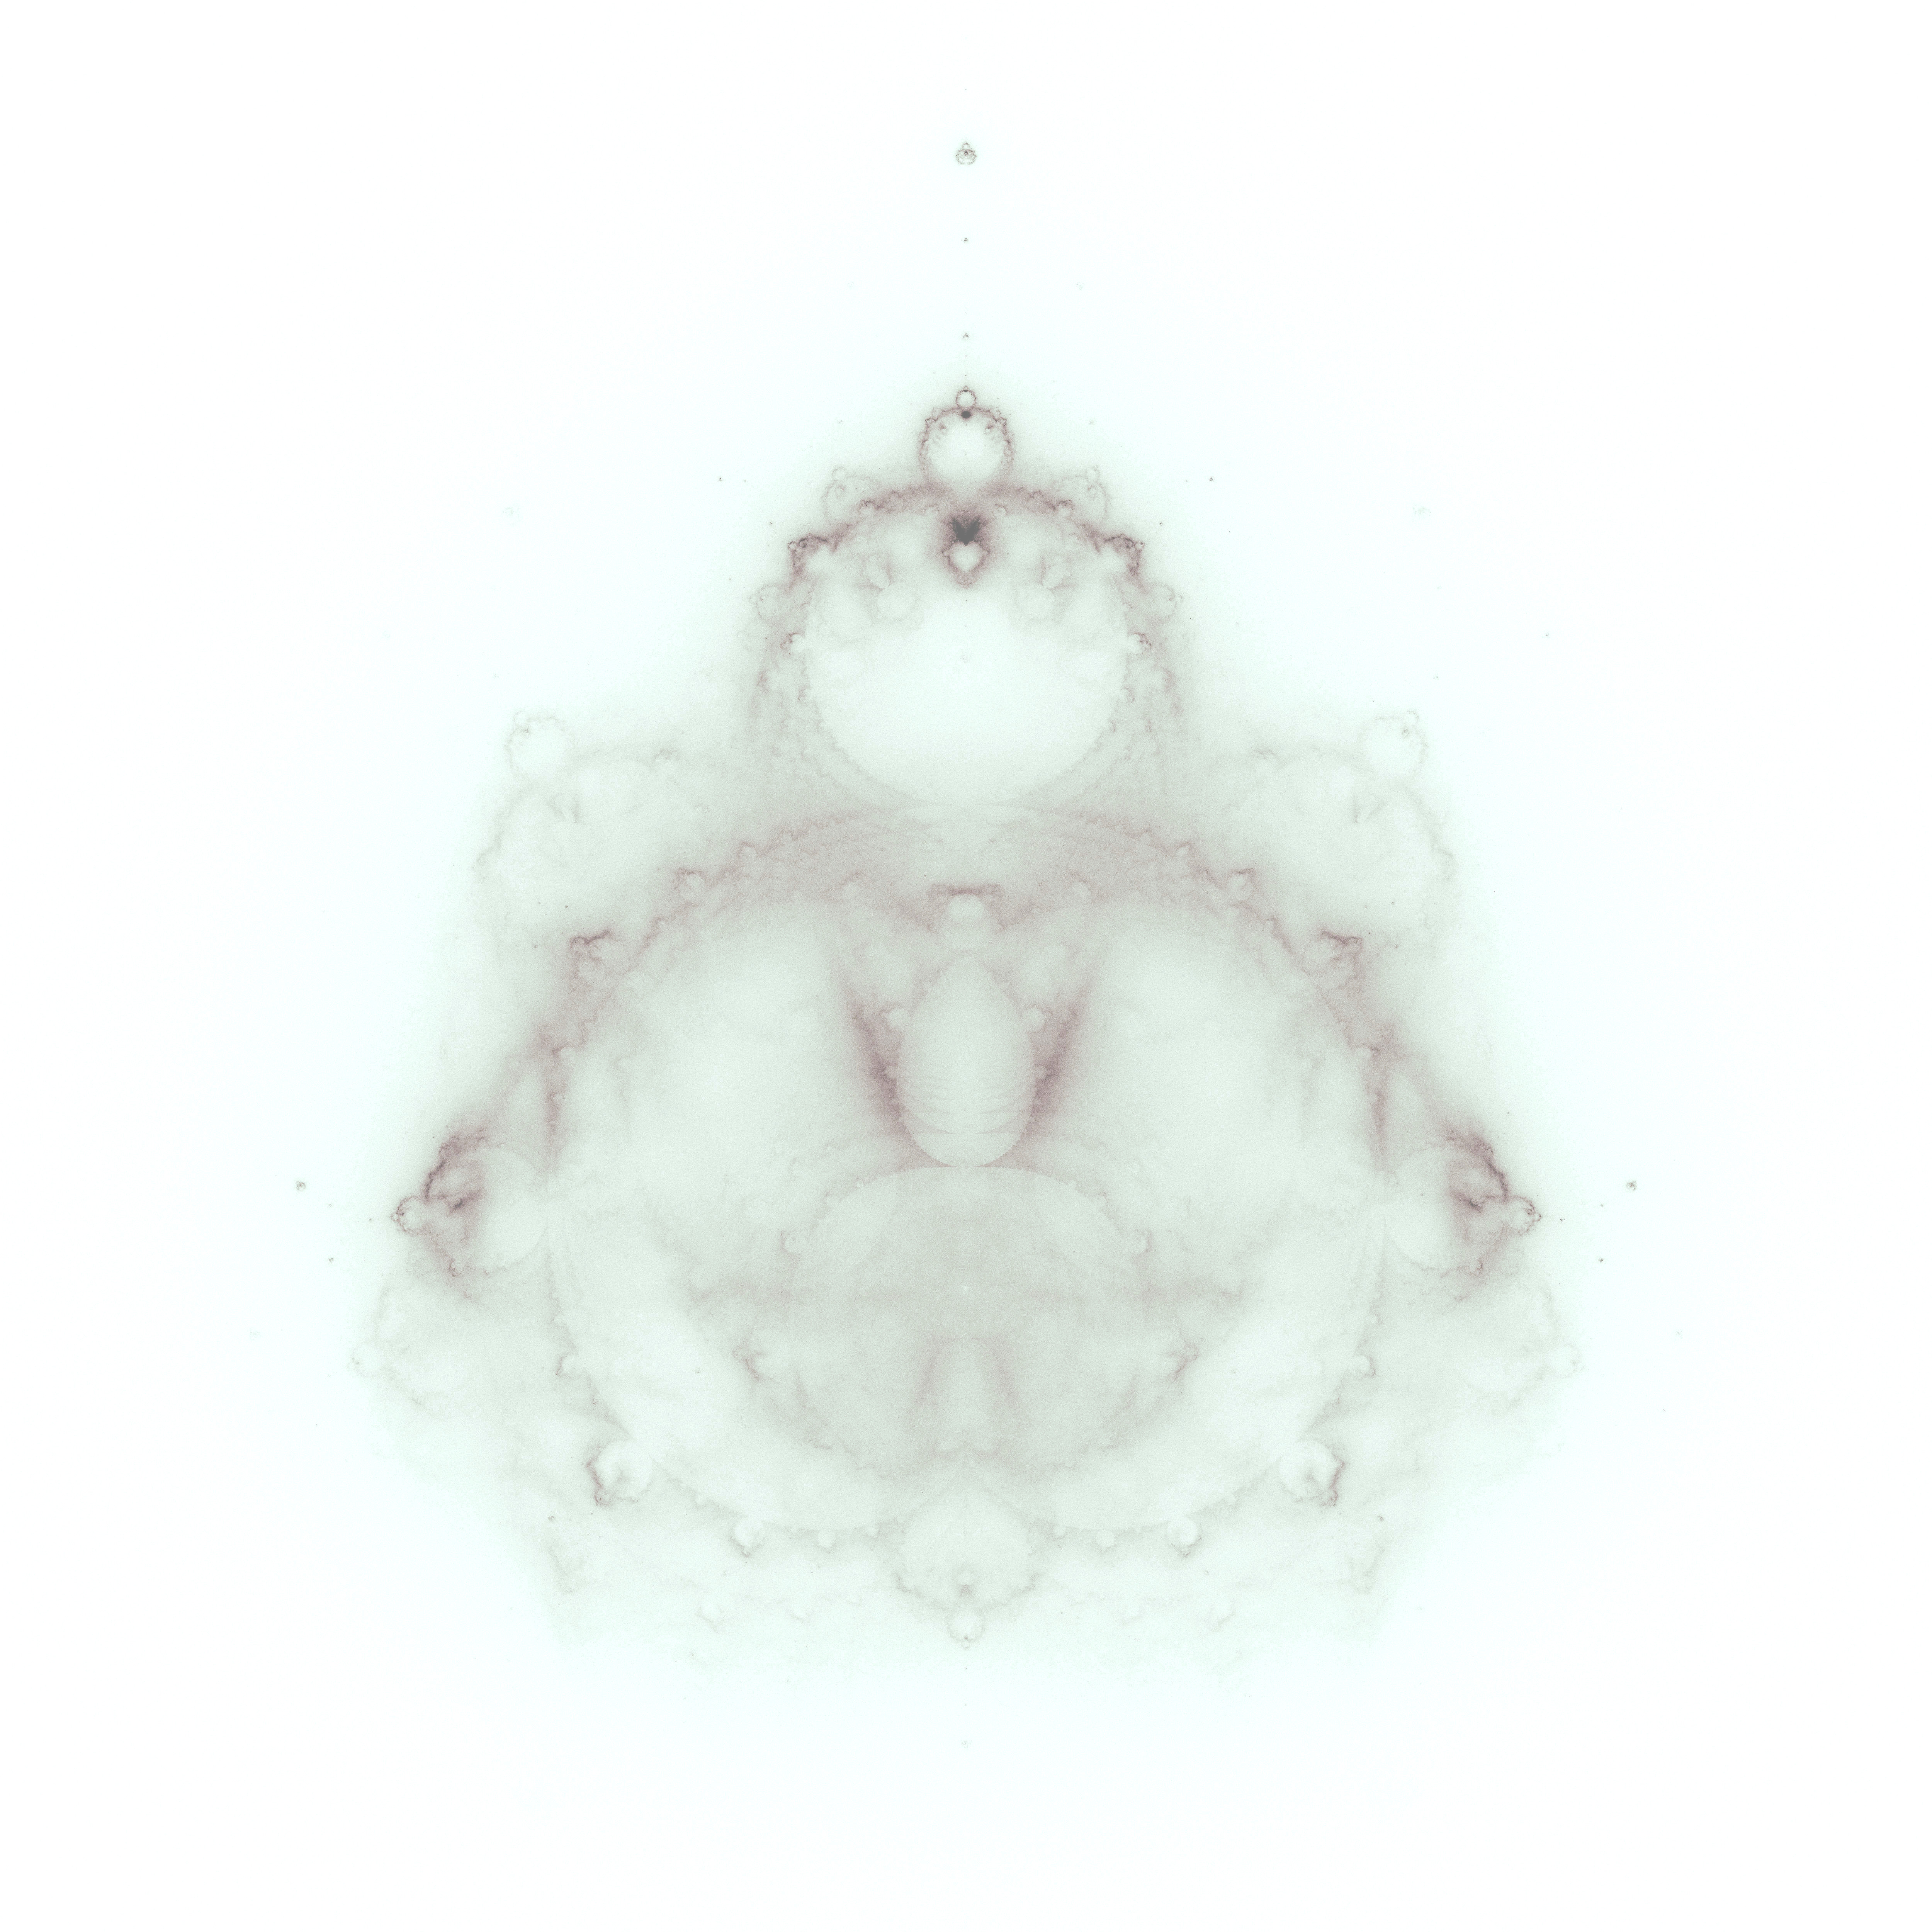
\includegraphics[height=\paperheight]{BuddhaBrot_light.jpg}}%
\begin{frame}
\begin{center}
{\Huge \color{hublue} \bf Thank you for the attention!}
\end{center}
\end{frame}

\end{document}

